% Options for packages loaded elsewhere
\PassOptionsToPackage{unicode}{hyperref}
\PassOptionsToPackage{hyphens}{url}
%
\documentclass[
]{article}
\usepackage{amsmath,amssymb}
\usepackage{iftex}
\ifPDFTeX
  \usepackage[T1]{fontenc}
  \usepackage[utf8]{inputenc}
  \usepackage{textcomp} % provide euro and other symbols
\else % if luatex or xetex
  \usepackage{unicode-math} % this also loads fontspec
  \defaultfontfeatures{Scale=MatchLowercase}
  \defaultfontfeatures[\rmfamily]{Ligatures=TeX,Scale=1}
\fi
\usepackage{lmodern}
\ifPDFTeX\else
  % xetex/luatex font selection
\fi
% Use upquote if available, for straight quotes in verbatim environments
\IfFileExists{upquote.sty}{\usepackage{upquote}}{}
\IfFileExists{microtype.sty}{% use microtype if available
  \usepackage[]{microtype}
  \UseMicrotypeSet[protrusion]{basicmath} % disable protrusion for tt fonts
}{}
\makeatletter
\@ifundefined{KOMAClassName}{% if non-KOMA class
  \IfFileExists{parskip.sty}{%
    \usepackage{parskip}
  }{% else
    \setlength{\parindent}{0pt}
    \setlength{\parskip}{6pt plus 2pt minus 1pt}}
}{% if KOMA class
  \KOMAoptions{parskip=half}}
\makeatother
\usepackage{xcolor}
\usepackage[margin=1in]{geometry}
\usepackage{color}
\usepackage{fancyvrb}
\newcommand{\VerbBar}{|}
\newcommand{\VERB}{\Verb[commandchars=\\\{\}]}
\DefineVerbatimEnvironment{Highlighting}{Verbatim}{commandchars=\\\{\}}
% Add ',fontsize=\small' for more characters per line
\usepackage{framed}
\definecolor{shadecolor}{RGB}{248,248,248}
\newenvironment{Shaded}{\begin{snugshade}}{\end{snugshade}}
\newcommand{\AlertTok}[1]{\textcolor[rgb]{0.94,0.16,0.16}{#1}}
\newcommand{\AnnotationTok}[1]{\textcolor[rgb]{0.56,0.35,0.01}{\textbf{\textit{#1}}}}
\newcommand{\AttributeTok}[1]{\textcolor[rgb]{0.13,0.29,0.53}{#1}}
\newcommand{\BaseNTok}[1]{\textcolor[rgb]{0.00,0.00,0.81}{#1}}
\newcommand{\BuiltInTok}[1]{#1}
\newcommand{\CharTok}[1]{\textcolor[rgb]{0.31,0.60,0.02}{#1}}
\newcommand{\CommentTok}[1]{\textcolor[rgb]{0.56,0.35,0.01}{\textit{#1}}}
\newcommand{\CommentVarTok}[1]{\textcolor[rgb]{0.56,0.35,0.01}{\textbf{\textit{#1}}}}
\newcommand{\ConstantTok}[1]{\textcolor[rgb]{0.56,0.35,0.01}{#1}}
\newcommand{\ControlFlowTok}[1]{\textcolor[rgb]{0.13,0.29,0.53}{\textbf{#1}}}
\newcommand{\DataTypeTok}[1]{\textcolor[rgb]{0.13,0.29,0.53}{#1}}
\newcommand{\DecValTok}[1]{\textcolor[rgb]{0.00,0.00,0.81}{#1}}
\newcommand{\DocumentationTok}[1]{\textcolor[rgb]{0.56,0.35,0.01}{\textbf{\textit{#1}}}}
\newcommand{\ErrorTok}[1]{\textcolor[rgb]{0.64,0.00,0.00}{\textbf{#1}}}
\newcommand{\ExtensionTok}[1]{#1}
\newcommand{\FloatTok}[1]{\textcolor[rgb]{0.00,0.00,0.81}{#1}}
\newcommand{\FunctionTok}[1]{\textcolor[rgb]{0.13,0.29,0.53}{\textbf{#1}}}
\newcommand{\ImportTok}[1]{#1}
\newcommand{\InformationTok}[1]{\textcolor[rgb]{0.56,0.35,0.01}{\textbf{\textit{#1}}}}
\newcommand{\KeywordTok}[1]{\textcolor[rgb]{0.13,0.29,0.53}{\textbf{#1}}}
\newcommand{\NormalTok}[1]{#1}
\newcommand{\OperatorTok}[1]{\textcolor[rgb]{0.81,0.36,0.00}{\textbf{#1}}}
\newcommand{\OtherTok}[1]{\textcolor[rgb]{0.56,0.35,0.01}{#1}}
\newcommand{\PreprocessorTok}[1]{\textcolor[rgb]{0.56,0.35,0.01}{\textit{#1}}}
\newcommand{\RegionMarkerTok}[1]{#1}
\newcommand{\SpecialCharTok}[1]{\textcolor[rgb]{0.81,0.36,0.00}{\textbf{#1}}}
\newcommand{\SpecialStringTok}[1]{\textcolor[rgb]{0.31,0.60,0.02}{#1}}
\newcommand{\StringTok}[1]{\textcolor[rgb]{0.31,0.60,0.02}{#1}}
\newcommand{\VariableTok}[1]{\textcolor[rgb]{0.00,0.00,0.00}{#1}}
\newcommand{\VerbatimStringTok}[1]{\textcolor[rgb]{0.31,0.60,0.02}{#1}}
\newcommand{\WarningTok}[1]{\textcolor[rgb]{0.56,0.35,0.01}{\textbf{\textit{#1}}}}
\usepackage{graphicx}
\makeatletter
\def\maxwidth{\ifdim\Gin@nat@width>\linewidth\linewidth\else\Gin@nat@width\fi}
\def\maxheight{\ifdim\Gin@nat@height>\textheight\textheight\else\Gin@nat@height\fi}
\makeatother
% Scale images if necessary, so that they will not overflow the page
% margins by default, and it is still possible to overwrite the defaults
% using explicit options in \includegraphics[width, height, ...]{}
\setkeys{Gin}{width=\maxwidth,height=\maxheight,keepaspectratio}
% Set default figure placement to htbp
\makeatletter
\def\fps@figure{htbp}
\makeatother
\setlength{\emergencystretch}{3em} % prevent overfull lines
\providecommand{\tightlist}{%
  \setlength{\itemsep}{0pt}\setlength{\parskip}{0pt}}
\setcounter{secnumdepth}{-\maxdimen} % remove section numbering
\ifLuaTeX
  \usepackage{selnolig}  % disable illegal ligatures
\fi
\IfFileExists{bookmark.sty}{\usepackage{bookmark}}{\usepackage{hyperref}}
\IfFileExists{xurl.sty}{\usepackage{xurl}}{} % add URL line breaks if available
\urlstyle{same}
\hypersetup{
  pdftitle={2025 NDMC Metagenome workshop},
  pdfauthor={Yincheng Chen},
  hidelinks,
  pdfcreator={LaTeX via pandoc}}

\title{2025 NDMC Metagenome workshop}
\author{\href{https://yinchengchen23.github.io/myCV/}{Yincheng Chen}}
\date{Created on March 26, 2025}

\begin{document}
\maketitle

{
\setcounter{tocdepth}{2}
\tableofcontents
}
\hypertarget{introduction-to-microbiota-data}{%
\section{Introduction to Microbiota
Data}\label{introduction-to-microbiota-data}}

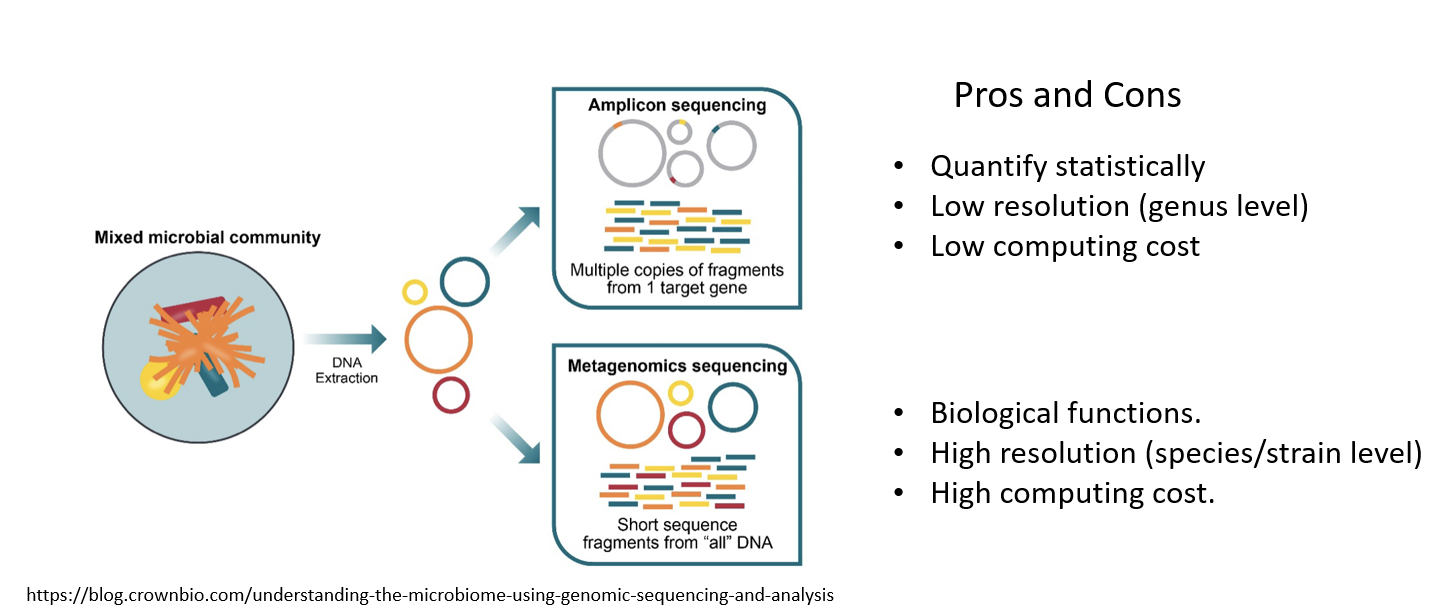
\includegraphics[width=0.8\textwidth,height=\textheight]{images/Fig1.png}

\hypertarget{practical-guide-to-microbiota-data}{%
\subsection{Practical guide to microbiota
data}\label{practical-guide-to-microbiota-data}}

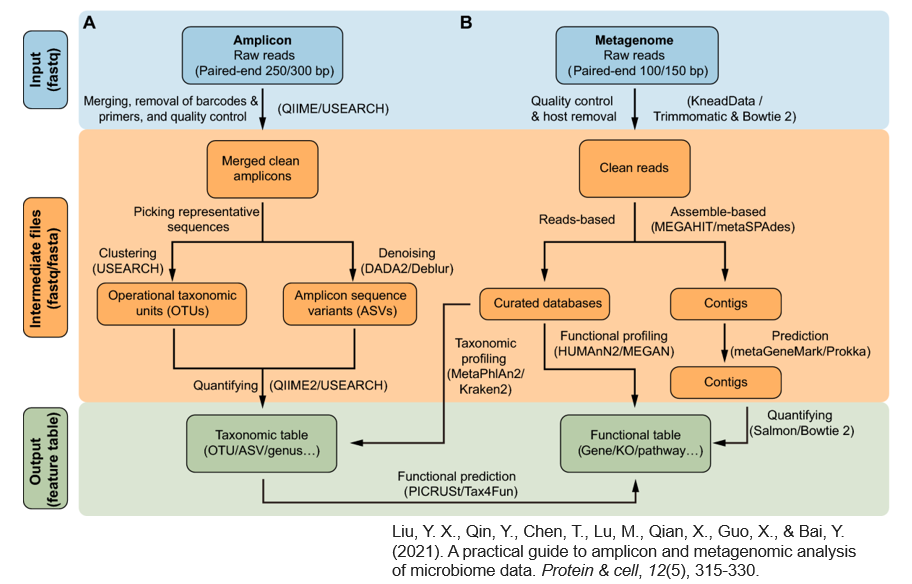
\includegraphics[width=0.8\textwidth,height=\textheight]{images/Fig2.png}

\hypertarget{s-rrna-amplicon}{%
\subsubsection{16s rRNA amplicon}\label{s-rrna-amplicon}}

Highly conserved in bacteria and archaea, but contains nine
hypervariable region V1-V9

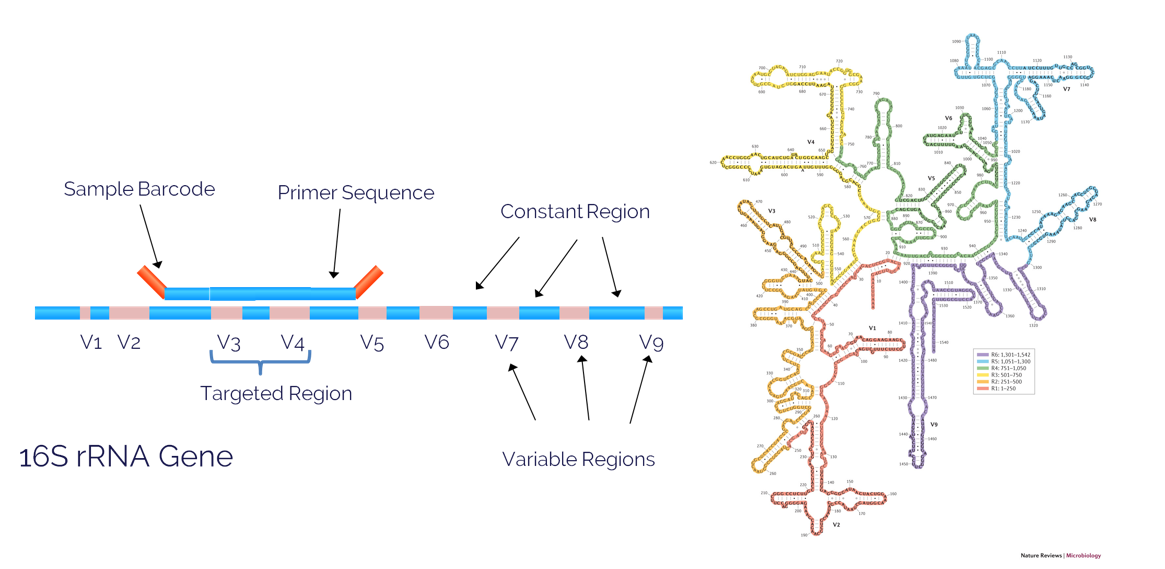
\includegraphics[width=0.8\textwidth,height=\textheight]{images/Fig3.png}

\hypertarget{sequence-process-for-amplicon-data}{%
\subsubsection{Sequence process for amplicon
data}\label{sequence-process-for-amplicon-data}}

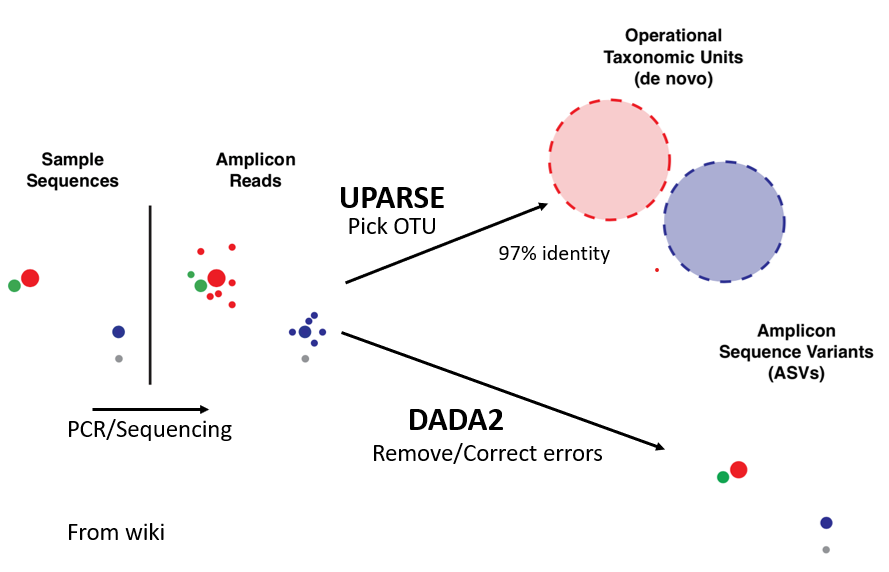
\includegraphics[width=0.8\textwidth,height=\textheight]{images/Fig4.png}

Reference database :

For bacteria

\begin{enumerate}
\def\labelenumi{\arabic{enumi}.}
\item
  \href{https://www.arb-silva.de/}{\textbf{SILVA} v138.2}, (2024, Nov.)
\item
  \href{https://zenodo.org/records/14168771}{\textbf{RDP} v19}, (2023,
  Aug.)
\item
  \href{https://www.nature.com/articles/s41587-023-01845-1}{\textbf{GreenGenes
  v2}}, (2024, Sep.)
\end{enumerate}

For fungi

\begin{itemize}
\tightlist
\item
  \href{https://unite.ut.ee/repository.php}{\textbf{UNITE v10}}, (2025,
  Feb.)
\end{itemize}

\hypertarget{pipeline-for-16s-rrna-amplicon}{%
\subsection{Pipeline for 16S rRNA
amplicon}\label{pipeline-for-16s-rrna-amplicon}}

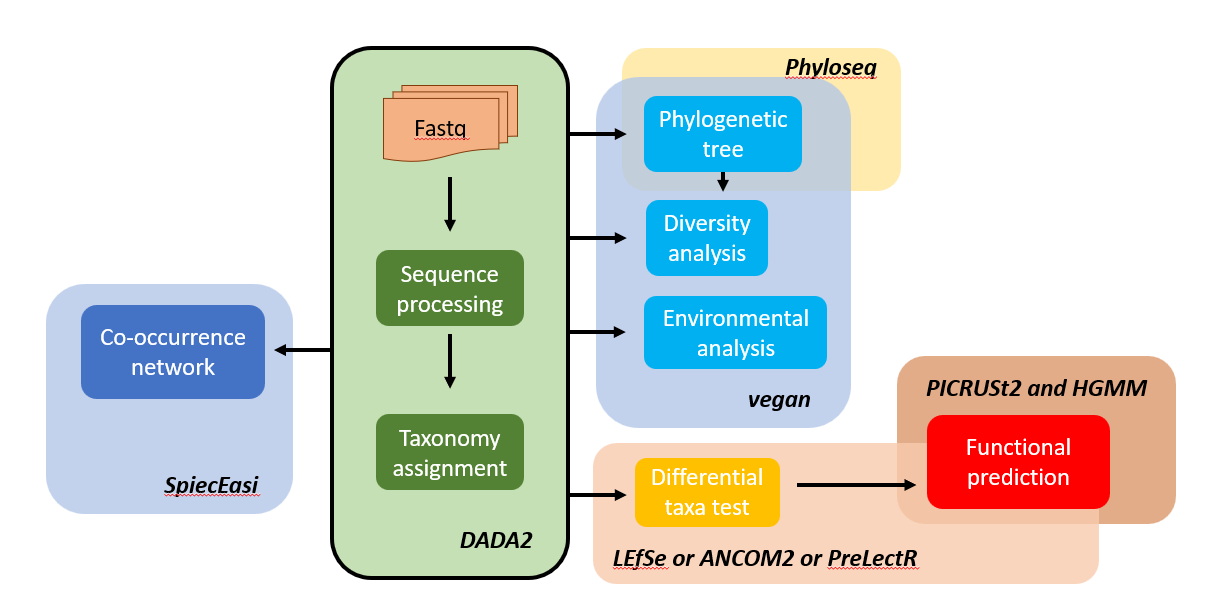
\includegraphics[width=0.8\textwidth,height=\textheight]{images/Fig5.png}

\hypertarget{fastq-format}{%
\paragraph{FASTQ format}\label{fastq-format}}

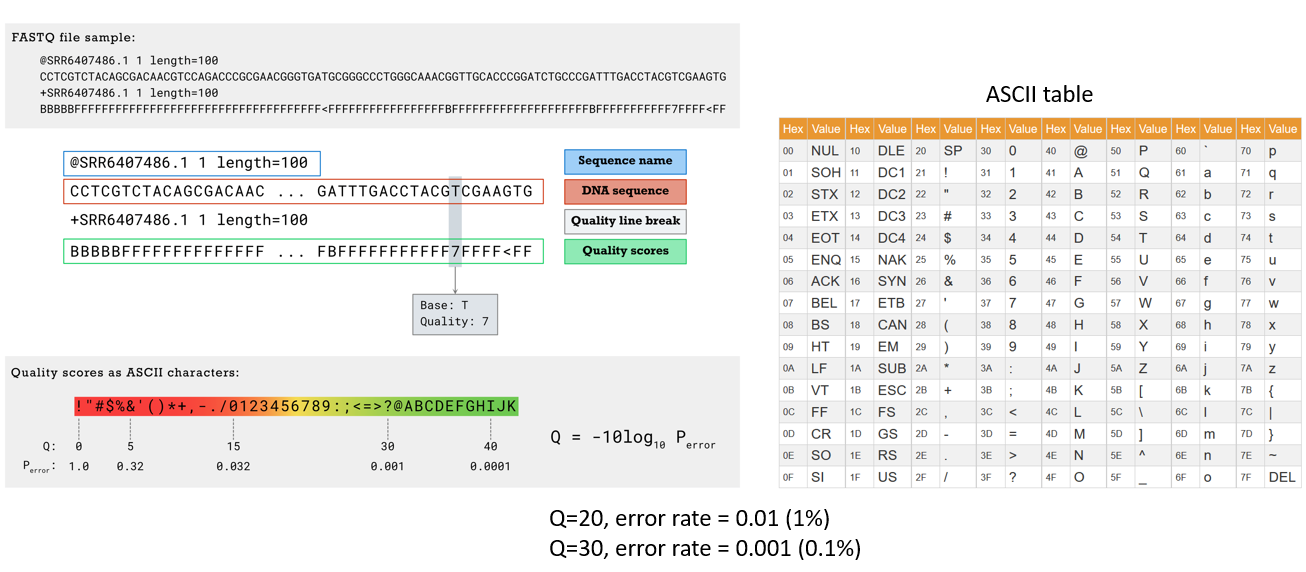
\includegraphics[width=0.8\textwidth,height=\textheight]{images/Fig6.png}

\begin{center}\rule{0.5\linewidth}{0.5pt}\end{center}

\hypertarget{dada2-pipeline-tutorial}{%
\subsection{DADA2 pipeline tutorial}\label{dada2-pipeline-tutorial}}

Please refer directly to the original
\href{https://benjjneb.github.io/dada2/tutorial.html}{page}

\hypertarget{step-1.-inspect-read-quality-profiles}{%
\subsubsection{Step 1. Inspect read quality
profiles}\label{step-1.-inspect-read-quality-profiles}}

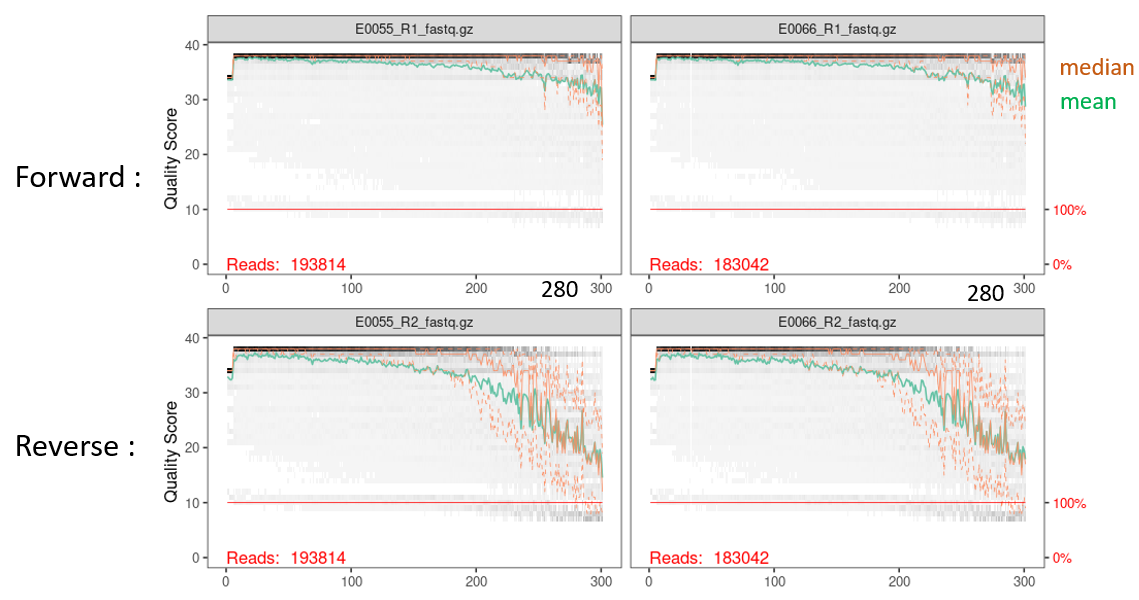
\includegraphics[width=1\textwidth,height=\textheight]{images/Fig7.png}

\hypertarget{step-2.-filter-and-trim}{%
\subsubsection{Step 2. Filter and trim}\label{step-2.-filter-and-trim}}

The key parameters for this step are \texttt{truncLen} and
\texttt{trimLeft}.

To prevent adapter sequence contamination, use \texttt{trimLeft} to
remove bases from the 5' end of the reads.

To ensure sequence quality, use \texttt{truncLen} to truncate reads
after assignment.

There are two important criteria to consider:

\begin{itemize}
\item
  After filtering, at least 80\% of the reads should be retained.
\item
  The V3-V4 region typically ranges from 360 to 420 nt in length, so the
  combined length of paired-end reads after truncation should be at
  least 400 nt to ensure sufficient overlap.
\end{itemize}

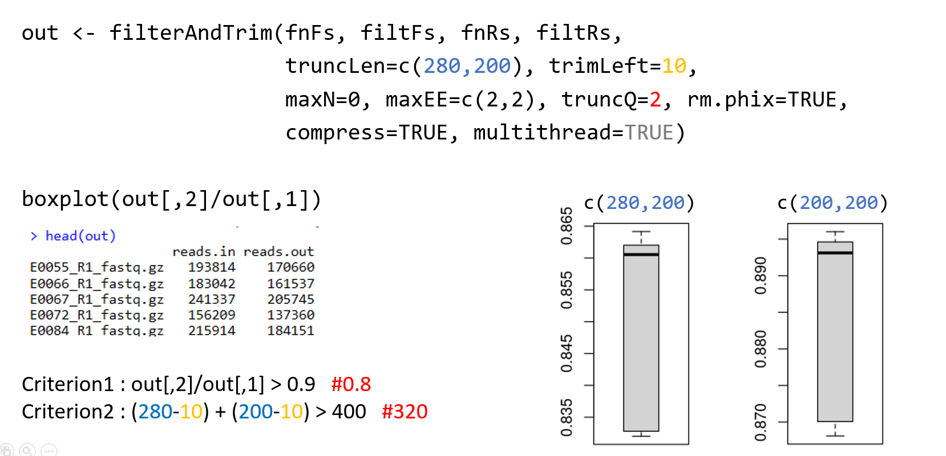
\includegraphics[width=0.8\textwidth,height=\textheight]{images/Fig8.png}

\hypertarget{step-3.-sequence-processing}{%
\subsubsection{Step 3. Sequence
processing}\label{step-3.-sequence-processing}}

Follow the standard procedures and verify the length of the merged
sequences.

\begin{Shaded}
\begin{Highlighting}[]
\CommentTok{\# Learn the Error Rates}
\NormalTok{errF }\OtherTok{\textless{}{-}} \FunctionTok{learnErrors}\NormalTok{(filtFs, }\AttributeTok{multithread=}\ConstantTok{TRUE}\NormalTok{)}
\NormalTok{...}

\CommentTok{\# Sample Inference}
\NormalTok{dadaFs }\OtherTok{\textless{}{-}} \FunctionTok{dada}\NormalTok{(filtFs, }\AttributeTok{err=}\NormalTok{errF, }\AttributeTok{multithread=}\ConstantTok{TRUE}\NormalTok{)}
\NormalTok{...}

\CommentTok{\# Merge paired reads}
\NormalTok{mergers }\OtherTok{\textless{}{-}} \FunctionTok{mergePairs}\NormalTok{(dadaFs, filtFs, dadaRs, filtRs, }\AttributeTok{verbose=}\ConstantTok{TRUE}\NormalTok{)}
\NormalTok{seqtab }\OtherTok{\textless{}{-}} \FunctionTok{makeSequenceTable}\NormalTok{(mergers)}
\FunctionTok{dim}\NormalTok{(seqtab) }\CommentTok{\# [n\_smaple, n\_ASVs]}

\CommentTok{\# Inspect distribution of sequence lengths}
\FunctionTok{hist}\NormalTok{(}\FunctionTok{nchar}\NormalTok{(}\FunctionTok{getSequences}\NormalTok{(seqtab)))}

\CommentTok{\# Remove chimeras}
\NormalTok{seqtab.nochim }\OtherTok{\textless{}{-}} \FunctionTok{removeBimeraDenovo}\NormalTok{(seqtab, }\AttributeTok{method=}\StringTok{"consensus"}\NormalTok{, }\AttributeTok{multithread=}\ConstantTok{TRUE}\NormalTok{, }\AttributeTok{verbose=}\ConstantTok{TRUE}\NormalTok{)}
\NormalTok{...}

\CommentTok{\# Assign taxonomy}
\NormalTok{taxa }\OtherTok{\textless{}{-}} \FunctionTok{assignTaxonomy}\NormalTok{(seqtab.nochim, }\StringTok{"\textasciitilde{}/tax/silva\_nr\_v132\_train\_set.fa.gz"}\NormalTok{, }\AttributeTok{multithread=}\ConstantTok{TRUE}\NormalTok{)}
\NormalTok{taxa }\OtherTok{\textless{}{-}} \FunctionTok{addSpecies}\NormalTok{(taxa, }\StringTok{"\textasciitilde{}/tax/silva\_species\_assignment\_v132.fa.gz"}\NormalTok{)}
\end{Highlighting}
\end{Shaded}

\hypertarget{step-4.-sample-qc}{%
\subsubsection{Step 4. Sample QC}\label{step-4.-sample-qc}}

\begin{Shaded}
\begin{Highlighting}[]
\NormalTok{getN }\OtherTok{\textless{}{-}} \ControlFlowTok{function}\NormalTok{(x) }\FunctionTok{sum}\NormalTok{(}\FunctionTok{getUniques}\NormalTok{(x))}
\NormalTok{track }\OtherTok{\textless{}{-}} \FunctionTok{cbind}\NormalTok{(out, }\FunctionTok{sapply}\NormalTok{(dadaFs, getN), }\FunctionTok{sapply}\NormalTok{(dadaRs, getN), }\FunctionTok{sapply}\NormalTok{(mergers, getN), }\FunctionTok{rowSums}\NormalTok{(seqtab.nochim))}
\FunctionTok{colnames}\NormalTok{(track) }\OtherTok{\textless{}{-}} \FunctionTok{c}\NormalTok{(}\StringTok{"input"}\NormalTok{, }\StringTok{"filtered"}\NormalTok{, }\StringTok{"denoisedF"}\NormalTok{, }\StringTok{"denoisedR"}\NormalTok{, }\StringTok{"merged"}\NormalTok{, }\StringTok{"nonchim"}\NormalTok{)}
\FunctionTok{rownames}\NormalTok{(track) }\OtherTok{\textless{}{-}}\NormalTok{ sample.names}
\NormalTok{mitochondria\_id }\OtherTok{\textless{}{-}} \FunctionTok{rownames}\NormalTok{(taxa)[taxa[,}\DecValTok{5}\NormalTok{] }\SpecialCharTok{\%in\%} \StringTok{"Mitochondria"}\NormalTok{]}
\NormalTok{unclassification\_id }\OtherTok{\textless{}{-}}\FunctionTok{rownames}\NormalTok{(taxa)[taxa[,}\DecValTok{1}\NormalTok{] }\SpecialCharTok{!=} \StringTok{"Bacteria"} \SpecialCharTok{|} \FunctionTok{is.na}\NormalTok{(taxa[,}\DecValTok{2}\NormalTok{])]}
\NormalTok{keep\_id }\OtherTok{\textless{}{-}} \FunctionTok{rownames}\NormalTok{(taxa)[}\SpecialCharTok{!}\FunctionTok{rownames}\NormalTok{(taxa) }\SpecialCharTok{\%in\%}\NormalTok{ mitochondria\_id}\ErrorTok{)}\NormalTok{]}
\NormalTok{get\_seqN }\OtherTok{\textless{}{-}} \ControlFlowTok{function}\NormalTok{(table,list)\{}
  \ControlFlowTok{if}\NormalTok{(}\FunctionTok{length}\NormalTok{(list) }\SpecialCharTok{==} \DecValTok{0}\NormalTok{) \{ }\FunctionTok{return}\NormalTok{(}\FunctionTok{rep}\NormalTok{(}\DecValTok{0}\NormalTok{,}\FunctionTok{nrow}\NormalTok{(table)))}
\NormalTok{  \} }\ControlFlowTok{else} \ControlFlowTok{if}\NormalTok{(}\FunctionTok{length}\NormalTok{(list) }\SpecialCharTok{\textgreater{}} \DecValTok{1}\NormalTok{) \{ }\FunctionTok{return}\NormalTok{(}\FunctionTok{rowSums}\NormalTok{(table[,list]))}
\NormalTok{  \} }\ControlFlowTok{else}\NormalTok{ \{ }\FunctionTok{return}\NormalTok{(}\FunctionTok{sapply}\NormalTok{(table[,list],sum))\}}
\NormalTok{\}}
\NormalTok{track }\OtherTok{\textless{}{-}} \FunctionTok{cbind}\NormalTok{(track, }\FunctionTok{get\_seqN}\NormalTok{(seqtab, mitochondria\_id), }\FunctionTok{get\_seqN}\NormalTok{(seqtab,keep\_id))}
\FunctionTok{colnames}\NormalTok{(track) }\OtherTok{\textless{}{-}}  \FunctionTok{c}\NormalTok{(}\StringTok{"input"}\NormalTok{, }\StringTok{"filtered"}\NormalTok{, }\StringTok{"denoisedF"}\NormalTok{, }\StringTok{"denoisedR"}\NormalTok{, }\StringTok{"merged"}\NormalTok{, }\StringTok{"nonchim"}\NormalTok{,}\StringTok{"mitochondria"}\NormalTok{,}\StringTok{"final"}\NormalTok{)}
\NormalTok{track }\OtherTok{\textless{}{-}}\NormalTok{ track[keep\_sample,]}
\NormalTok{keep\_sample }\OtherTok{\textless{}{-}} \FunctionTok{rownames}\NormalTok{(track)[track[,}\DecValTok{8}\NormalTok{]}\SpecialCharTok{/}\NormalTok{track[,}\DecValTok{6}\NormalTok{] }\SpecialCharTok{\textgreater{}} \FloatTok{0.5}\NormalTok{]  }\CommentTok{\# remove the sample with host contamination \textgreater{} 50\%}
\NormalTok{seqtab }\OtherTok{\textless{}{-}}\NormalTok{ seqtab[keep\_sample,keep\_id]}
\NormalTok{nozeroASV }\OtherTok{\textless{}{-}} \FunctionTok{colnames}\NormalTok{(seqtab)[}\FunctionTok{colSums}\NormalTok{(seqtab) }\SpecialCharTok{\textgreater{}} \DecValTok{0}\NormalTok{]}
\NormalTok{seqtab }\OtherTok{\textless{}{-}}\NormalTok{ seqtab[,nozeroASV]}
\NormalTok{taxa }\OtherTok{\textless{}{-}}\NormalTok{ taxa[nozeroASV,]}
\end{Highlighting}
\end{Shaded}

\hypertarget{step-5.-serial-number-and-output}{%
\subsubsection{Step 5. Serial number and
output}\label{step-5.-serial-number-and-output}}

\begin{Shaded}
\begin{Highlighting}[]
\FunctionTok{source}\NormalTok{(}\StringTok{"source/utils.R"}\NormalTok{)}
\NormalTok{output\_path }\OtherTok{\textless{}{-}} \StringTok{\textquotesingle{}\textasciitilde{}/dada2\_output\textquotesingle{}}
\FunctionTok{DADA2Adapter}\NormalTok{(seqtab.nochim, taxa, output\_path)  }\CommentTok{\# DADA2Adapter function is sourced from utils.R}
\FunctionTok{dir}\NormalTok{(output\_path)}

\NormalTok{data }\OtherTok{\textless{}{-}} \FunctionTok{read.csv}\NormalTok{(}\FunctionTok{paste0}\NormalTok{(output\_path,}\StringTok{\textquotesingle{}/ASV\_table.txt\textquotesingle{}}\NormalTok{), }\AttributeTok{sep =} \StringTok{\textquotesingle{}}\SpecialCharTok{\textbackslash{}t}\StringTok{\textquotesingle{}}\NormalTok{)}
\NormalTok{taxa }\OtherTok{\textless{}{-}} \FunctionTok{read.csv}\NormalTok{(}\FunctionTok{paste0}\NormalTok{(output\_path,}\StringTok{\textquotesingle{}/ASV\_taxa\_table.txt\textquotesingle{}}\NormalTok{), }\AttributeTok{sep =} \StringTok{\textquotesingle{}}\SpecialCharTok{\textbackslash{}t}\StringTok{\textquotesingle{}}\NormalTok{)}
\end{Highlighting}
\end{Shaded}

\hypertarget{step-6.-phylogenetic-tree-building-1}{%
\subsubsection{Step 6. Phylogenetic tree building
(1)}\label{step-6.-phylogenetic-tree-building-1}}

The phylogenetic tree can be directly constructed using
\texttt{DECIPHER}. However, fitting a GTR model is time-consuming
(5hr-10hr), and installing \texttt{DECIPHER} can be challenging.

\begin{Shaded}
\begin{Highlighting}[]
\FunctionTok{library}\NormalTok{(dada2)}
\FunctionTok{library}\NormalTok{(DECIPHER)}
\FunctionTok{library}\NormalTok{(phangorn)}

\NormalTok{seqs }\OtherTok{\textless{}{-}} \FunctionTok{getSequences}\NormalTok{(seqtab.nochim)}
\NormalTok{magnitude }\OtherTok{\textless{}{-}} \FunctionTok{ceiling}\NormalTok{(}\FunctionTok{log10}\NormalTok{(}\FunctionTok{ncol}\NormalTok{(seqtab.nochim)))}
\NormalTok{ASVID }\OtherTok{\textless{}{-}} \FunctionTok{sprintf}\NormalTok{(}\FunctionTok{paste0}\NormalTok{(}\StringTok{"ASV\%0"}\NormalTok{, magnitude, }\StringTok{"d"}\NormalTok{), }\DecValTok{1}\SpecialCharTok{:}\NormalTok{n\_ASVs)}


\FunctionTok{names}\NormalTok{(seqs) }\OtherTok{\textless{}{-}}\NormalTok{ ASVID}
\NormalTok{alignment }\OtherTok{\textless{}{-}} \FunctionTok{AlignSeqs}\NormalTok{(}\FunctionTok{DNAStringSet}\NormalTok{(seqs), }\AttributeTok{anchor=}\ConstantTok{NA}\NormalTok{,}\AttributeTok{verbose=}\ConstantTok{TRUE}\NormalTok{)}

\NormalTok{phangAlign }\OtherTok{\textless{}{-}} \FunctionTok{phyDat}\NormalTok{(}\FunctionTok{as}\NormalTok{(alignment, }\StringTok{"matrix"}\NormalTok{), }\AttributeTok{type=}\StringTok{"DNA"}\NormalTok{)}
\NormalTok{dm }\OtherTok{\textless{}{-}} \FunctionTok{dist.ml}\NormalTok{(phangAlign)}
\NormalTok{treeNJ }\OtherTok{\textless{}{-}} \FunctionTok{NJ}\NormalTok{(dm)}
\NormalTok{fit }\OtherTok{=} \FunctionTok{pml}\NormalTok{(treeNJ, }\AttributeTok{data=}\NormalTok{phangAlign)}
\NormalTok{fitGTR }\OtherTok{\textless{}{-}} \FunctionTok{update}\NormalTok{(fit, }\AttributeTok{k=}\DecValTok{4}\NormalTok{, }\AttributeTok{inv=}\FloatTok{0.2}\NormalTok{)}
\NormalTok{fitGTR }\OtherTok{\textless{}{-}} \FunctionTok{optim.pml}\NormalTok{(fitGTR, }\AttributeTok{model=}\StringTok{"GTR"}\NormalTok{, }\AttributeTok{optInv=}\ConstantTok{TRUE}\NormalTok{, }\AttributeTok{optGamma=}\ConstantTok{TRUE}\NormalTok{,}
                    \AttributeTok{rearrangement =} \StringTok{"stochastic"}\NormalTok{, }\AttributeTok{control =} \FunctionTok{pml.control}\NormalTok{(}\AttributeTok{trace =} \DecValTok{0}\NormalTok{))}
\NormalTok{fitGTR}\SpecialCharTok{$}\NormalTok{tree}

\FunctionTok{write.tree}\NormalTok{(fitGTR}\SpecialCharTok{$}\NormalTok{tree, }\AttributeTok{file =} \FunctionTok{paste0}\NormalTok{(output\_path,}\StringTok{\textquotesingle{}/ASV.tree\textquotesingle{}}\NormalTok{), }\AttributeTok{append =} \ConstantTok{FALSE}\NormalTok{,}
           \AttributeTok{digits =} \DecValTok{10}\NormalTok{, }\AttributeTok{tree.names =} \ConstantTok{FALSE}\NormalTok{)}
\end{Highlighting}
\end{Shaded}

\hypertarget{step-6.-phylogenetic-tree-building-2}{%
\subsubsection{Step 6. Phylogenetic tree building
(2)}\label{step-6.-phylogenetic-tree-building-2}}

So we provider an alternative approach. Since 16S ribosomal sequences
contained the non-coding sequence and secondary structure, the alignment
method was considered. We suggest to use
\href{http://eddylab.org/software/ssu-align/}{ssu-align} to do alignment
for phylogenetic inference. The detailed process is as follows.

\begin{Shaded}
\begin{Highlighting}[]
\CommentTok{\# ssu{-}align installation}
\ExtensionTok{$}\NormalTok{ wget eddylab.org/software/ssu{-}align/ssu{-}align{-}0.1.1.tar.gz}\KeywordTok{;}
\ExtensionTok{$}\NormalTok{ tar xfz ssu{-}align{-}0.1.1.tar.gz}
\ExtensionTok{$}\NormalTok{ cd ssu{-}align{-}0.1.1}
\ExtensionTok{$}\NormalTok{ ./configure}
\ExtensionTok{$}\NormalTok{ make}
\CommentTok{\# install the man pages and programs in system{-}wide directories:}
\ExtensionTok{$}\NormalTok{ make install}

\ExtensionTok{$}\NormalTok{ export PATH=}\StringTok{"}\VariableTok{$PATH}\StringTok{:/usr/local/bin"}
\ExtensionTok{$}\NormalTok{ export MANPATH=}\StringTok{"}\VariableTok{$MANPATH}\StringTok{:/usr/local/share/man"}
\ExtensionTok{$}\NormalTok{ export SSUALIGNDIR=}\StringTok{"/usr/local/share/ssu{-}align{-}0.1.1"}

\CommentTok{\# conduct SSU{-}alignment}
\ExtensionTok{$}\NormalTok{ cd \textasciitilde{}/Course/NDMC\_2025/tmp}
\ExtensionTok{$}\NormalTok{ ssu{-}align ASV.fasta ssuout}
\ExtensionTok{$}\NormalTok{ cd ssuout}
\end{Highlighting}
\end{Shaded}

The alignment result is generated in
\texttt{ssuout/ssuout.bacteria.stk}.

We can convert the \texttt{.stk} file to FASTA format using
\texttt{alignment\_transform.R}, located in the source folder.

\begin{Shaded}
\begin{Highlighting}[]
\ExtensionTok{$}\NormalTok{ Rscript }\AttributeTok{{-}{-}vanilla}\NormalTok{ \textasciitilde{}/Course/NDMC\_2025/source/alignment\_transform.R \textasciitilde{}/Course/NDMC\_2025/tmp/ssuout/ssuout.bacteria.stk \textasciitilde{}/Course/NDMC\_2025/tmp/ssuout/ssu\_aligned.fasta}
\end{Highlighting}
\end{Shaded}

In order to shorten the processing time, we use the
\href{http://www.microbesonline.org/fasttree/}{FastTree} for
maximum-likelihood phylogenetic tree completion. If time is available,
\href{https://cme.h-its.org/exelixis/web/software/raxml/}{RAxML} is
suggested to get the better quality tree.

\begin{Shaded}
\begin{Highlighting}[]
\ExtensionTok{$}\NormalTok{ cd \textasciitilde{}/Course/NDMC\_2025/tmp}
\ExtensionTok{$}\NormalTok{ \textasciitilde{}/bin/FastTree }\AttributeTok{{-}gtr} \AttributeTok{{-}nt}\NormalTok{ ./ssuout/ssu\_align.fasta }\OperatorTok{\textgreater{}}\NormalTok{ ./ASV.tree}
\end{Highlighting}
\end{Shaded}

\hypertarget{diversity-analysis}{%
\section{Diversity Analysis}\label{diversity-analysis}}

The fecal microbiota data which from PRJEB6070
\href{https://pubmed.ncbi.nlm.nih.gov/25432777/}{(Zeller et al., 2016)}
is used in this demonstration. We subsetted this dataset, including 20
patients each from the normal and cancer groups, and used the DADA2
pipeline to complete the analysis up to the taxonomic assignment step.

Please ensure that the packages listed in \texttt{prep\_help.R} are
installed.

\begin{Shaded}
\begin{Highlighting}[]
\FunctionTok{library}\NormalTok{(dada2)}
\FunctionTok{library}\NormalTok{(dplyr)}
\FunctionTok{library}\NormalTok{(DECIPHER)}
\FunctionTok{library}\NormalTok{(phangorn)}
\FunctionTok{library}\NormalTok{(matrixStats)}
\FunctionTok{library}\NormalTok{(ggpubr)}
\FunctionTok{library}\NormalTok{(ggplot2)}
\FunctionTok{library}\NormalTok{(picante)}
\FunctionTok{library}\NormalTok{(phyloseq)}
\FunctionTok{library}\NormalTok{(patchwork)}
\FunctionTok{library}\NormalTok{(rstatix)}
\FunctionTok{library}\NormalTok{(tidyverse)}
\FunctionTok{library}\NormalTok{(vegan)}
\FunctionTok{library}\NormalTok{(scales)}

\FunctionTok{source}\NormalTok{(}\StringTok{"source/utils.R"}\NormalTok{)}
\end{Highlighting}
\end{Shaded}

\begin{Shaded}
\begin{Highlighting}[]
\NormalTok{dataset\_path }\OtherTok{\textless{}{-}} \StringTok{"\textasciitilde{}/Course/NDMC\_2025/data/Zeller\_CRC.RData"}
\FunctionTok{load}\NormalTok{(dataset\_path)}
\FunctionTok{print}\NormalTok{(}\FunctionTok{ls}\NormalTok{())}
\DocumentationTok{\#\#  [1] "assignModul"       "DADA2Adapter"      "dataset\_path"     }
\DocumentationTok{\#\#  [4] "get\_composition"   "ggrare"            "GMMviz"           }
\DocumentationTok{\#\#  [7] "LEfSe\_preparation" "make\_edgetable"    "make\_net"         }
\DocumentationTok{\#\# [10] "make\_nodetable"    "meta"              "phyloseq\_to\_edgeR"}
\DocumentationTok{\#\# [13] "seqtab"            "seqtab.nochim"     "taxa"             }
\DocumentationTok{\#\# [16] "track"             "track\_ab"          "track\_ta"}

\CommentTok{\# Check patients condition}
\FunctionTok{print}\NormalTok{(}\FunctionTok{table}\NormalTok{(meta}\SpecialCharTok{$}\NormalTok{Class))}
\DocumentationTok{\#\# }
\DocumentationTok{\#\# Cancer Normal }
\DocumentationTok{\#\#     20     20}
\FunctionTok{print}\NormalTok{(}\FunctionTok{table}\NormalTok{(meta}\SpecialCharTok{$}\NormalTok{diagnosis))}
\DocumentationTok{\#\# }
\DocumentationTok{\#\# Adenoma  Cancer  Normal }
\DocumentationTok{\#\#       6      20      14}

\CommentTok{\# The clinical factor for time{-}to{-}event testing}
\NormalTok{meta}\SpecialCharTok{$}\NormalTok{event }\OtherTok{\textless{}{-}} \FunctionTok{ifelse}\NormalTok{(meta}\SpecialCharTok{$}\NormalTok{Class }\SpecialCharTok{==} \StringTok{\textquotesingle{}Cancer\textquotesingle{}}\NormalTok{, }\DecValTok{1}\NormalTok{, }\DecValTok{0}\NormalTok{)  }\CommentTok{\# as events}
\NormalTok{meta}\SpecialCharTok{$}\NormalTok{duration }\OtherTok{\textless{}{-}}\NormalTok{ meta}\SpecialCharTok{$}\NormalTok{age                           }\CommentTok{\# as duration}
\end{Highlighting}
\end{Shaded}

We designed the \texttt{DADA2Adapter} function to bridge the data into
the \texttt{PreLect} pipeline.

\begin{Shaded}
\begin{Highlighting}[]
\CommentTok{\# set the working  directory }
\NormalTok{output\_path }\OtherTok{\textless{}{-}} \StringTok{\textquotesingle{}/home/yincheng23/Course/NDMC\_2025/tmp\textquotesingle{}}

\CommentTok{\# generate the raw count table, taxa table and ASV sequence fasta}
\FunctionTok{DADA2Adapter}\NormalTok{(seqtab.nochim, taxa, output\_path) }\CommentTok{\# DADA2Adapter function is sourced from utils.R}
\FunctionTok{dir}\NormalTok{(output\_path)}
\DocumentationTok{\#\# [1] "ASV\_table.txt"      "ASV\_taxa\_table.txt" "ASV.fasta"         }
\DocumentationTok{\#\# [4] "ASV.tree"           "for\_PICRUSt2.tsv"   "LEfSe\_tmp"         }
\DocumentationTok{\#\# [7] "PICRUSt2"           "PreLect\_tmp"        "ssuout"}

\CommentTok{\# load the data we need}
\NormalTok{data }\OtherTok{\textless{}{-}} \FunctionTok{read.csv}\NormalTok{(}\FunctionTok{paste0}\NormalTok{(output\_path,}\StringTok{\textquotesingle{}/ASV\_table.txt\textquotesingle{}}\NormalTok{), }\AttributeTok{sep =} \StringTok{\textquotesingle{}}\SpecialCharTok{\textbackslash{}t}\StringTok{\textquotesingle{}}\NormalTok{)}
\NormalTok{taxa }\OtherTok{\textless{}{-}} \FunctionTok{read.csv}\NormalTok{(}\FunctionTok{paste0}\NormalTok{(output\_path,}\StringTok{\textquotesingle{}/ASV\_taxa\_table.txt\textquotesingle{}}\NormalTok{), }\AttributeTok{sep =} \StringTok{\textquotesingle{}}\SpecialCharTok{\textbackslash{}t}\StringTok{\textquotesingle{}}\NormalTok{)}
\NormalTok{taxa[}\FunctionTok{is.na}\NormalTok{(taxa)] }\OtherTok{\textless{}{-}} \StringTok{"unidentified"}
\end{Highlighting}
\end{Shaded}

\hypertarget{alpha-diversity}{%
\subsection{Alpha diversity}\label{alpha-diversity}}

Alpha diversity describes the species diversity within a community.

\hypertarget{rarefaction-normalization}{%
\subsubsection{Rarefaction
normalization}\label{rarefaction-normalization}}

Since various range of sequencing depth in data, we usually conduct the
rarefaction normalization to `fairly' compare the diversity metrics.

\begin{Shaded}
\begin{Highlighting}[]
\CommentTok{\# Rarefaction curve}
\NormalTok{ASV }\OtherTok{=} \FunctionTok{otu\_table}\NormalTok{(data, }\AttributeTok{taxa\_are\_rows =} \ConstantTok{TRUE}\NormalTok{)}
\NormalTok{TAX }\OtherTok{=} \FunctionTok{tax\_table}\NormalTok{(}\FunctionTok{as.matrix}\NormalTok{(taxa))}
\NormalTok{physeq }\OtherTok{=} \FunctionTok{phyloseq}\NormalTok{(ASV, TAX)}
\NormalTok{sampledata }\OtherTok{=} \FunctionTok{sample\_data}\NormalTok{(meta)}
\NormalTok{physeq }\OtherTok{=} \FunctionTok{merge\_phyloseq}\NormalTok{(physeq, sampledata)}

\NormalTok{min\_depth }\OtherTok{\textless{}{-}} \FunctionTok{min}\NormalTok{(}\FunctionTok{colSums}\NormalTok{(data))}
\FunctionTok{print}\NormalTok{(min\_depth)}
\end{Highlighting}
\end{Shaded}

\begin{verbatim}
## [1] 68528
\end{verbatim}

\begin{Shaded}
\begin{Highlighting}[]
\CommentTok{\# ggrare function is sourced from utils.R}
\FunctionTok{ggrare}\NormalTok{(physeq, }\AttributeTok{step =} \DecValTok{1500}\NormalTok{, }\AttributeTok{colour =} \StringTok{"Class"}\NormalTok{, }\AttributeTok{se =} \ConstantTok{FALSE}\NormalTok{) }\SpecialCharTok{+}
  \FunctionTok{scale\_colour\_brewer}\NormalTok{(}\AttributeTok{palette=}\StringTok{"Set1"}\NormalTok{) }\SpecialCharTok{+}
  \FunctionTok{geom\_vline}\NormalTok{(}\AttributeTok{xintercept =}\NormalTok{ min\_depth, }\AttributeTok{linetype =} \StringTok{\textquotesingle{}dotdash\textquotesingle{}}\NormalTok{) }\SpecialCharTok{+} 
  \FunctionTok{theme}\NormalTok{(}\AttributeTok{axis.line =} \FunctionTok{element\_line}\NormalTok{(}\AttributeTok{linetype =} \DecValTok{1}\NormalTok{,}\AttributeTok{colour =} \StringTok{\textquotesingle{}black\textquotesingle{}}\NormalTok{),}
  \AttributeTok{panel.background =} \FunctionTok{element\_rect}\NormalTok{(}\FunctionTok{I}\NormalTok{(}\DecValTok{0}\NormalTok{)),}
  \AttributeTok{panel.grid.major =} \FunctionTok{element\_line}\NormalTok{(}\AttributeTok{colour =} \ConstantTok{NA}\NormalTok{),}
  \AttributeTok{panel.grid.minor =} \FunctionTok{element\_line}\NormalTok{(}\AttributeTok{colour =} \ConstantTok{NA}\NormalTok{))}
\end{Highlighting}
\end{Shaded}

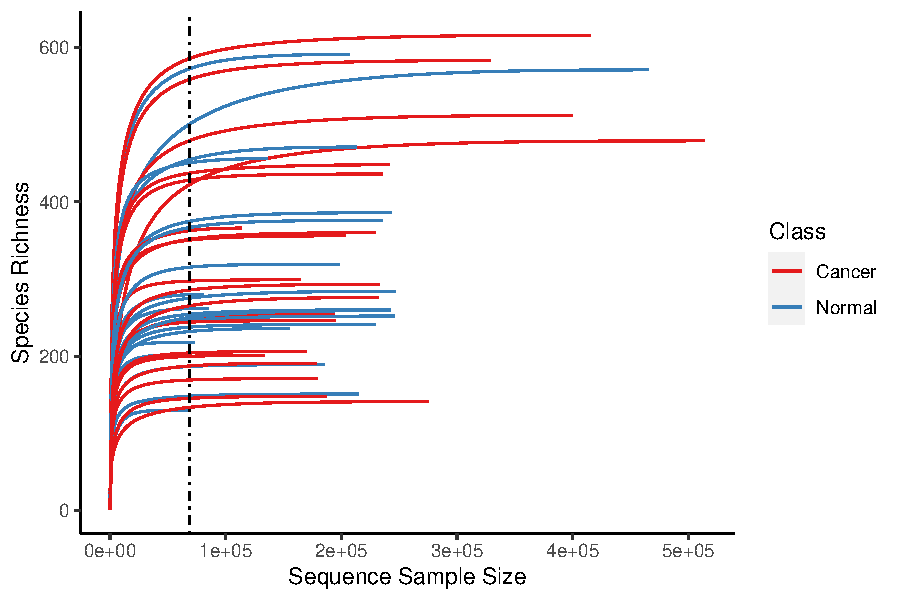
\includegraphics{workshop_files/figure-latex/unnamed-chunk-13-1.pdf}

The upper picture show the library size vs.~number of observed species,
in rarefaction process, we limited the all samples in minimum depth
\textbf{(black dotdash)}, and then randomly discarding reads from larger
samples until the number of remaining samples is equal to this threshold

\begin{Shaded}
\begin{Highlighting}[]
\CommentTok{\# Rarefaction}
\FunctionTok{print}\NormalTok{(}\FunctionTok{colSums}\NormalTok{(data)[}\DecValTok{1}\SpecialCharTok{:}\DecValTok{16}\NormalTok{])}
\DocumentationTok{\#\# ERR475473 ERR475476 ERR475478 ERR475480 ERR475483 ERR475484 ERR475485 ERR475493 }
\DocumentationTok{\#\#     73475    155494    207049     68528     70074     85513     80933    203534 }
\DocumentationTok{\#\# ERR475500 ERR475504 ERR475513 ERR475518 ERR475521 ERR475527 ERR475528 ERR475529 }
\DocumentationTok{\#\#    514255    465384    415085    242616    399663    328836    136463    133480}
\NormalTok{min }\OtherTok{\textless{}{-}} \FunctionTok{min}\NormalTok{(}\FunctionTok{colSums}\NormalTok{(data))}
\NormalTok{data\_rarefied }\OtherTok{\textless{}{-}} \FunctionTok{t}\NormalTok{(}\FunctionTok{rrarefy}\NormalTok{(}\FunctionTok{t}\NormalTok{(data), min))}
\DocumentationTok{\#\# Warning in rrarefy(t(data), min): function should be used for observed counts,}
\DocumentationTok{\#\# but smallest count is 2}
\NormalTok{data\_rarefied }\OtherTok{\textless{}{-}}\NormalTok{ data\_rarefied[}\FunctionTok{rowSums}\NormalTok{(data\_rarefied) }\SpecialCharTok{\textgreater{}} \DecValTok{0}\NormalTok{,]}
\FunctionTok{print}\NormalTok{(}\FunctionTok{colSums}\NormalTok{(data\_rarefied)[}\DecValTok{1}\SpecialCharTok{:}\DecValTok{16}\NormalTok{])}
\DocumentationTok{\#\# ERR475473 ERR475476 ERR475478 ERR475480 ERR475483 ERR475484 ERR475485 ERR475493 }
\DocumentationTok{\#\#     68528     68528     68528     68528     68528     68528     68528     68528 }
\DocumentationTok{\#\# ERR475500 ERR475504 ERR475513 ERR475518 ERR475521 ERR475527 ERR475528 ERR475529 }
\DocumentationTok{\#\#     68528     68528     68528     68528     68528     68528     68528     68528}
\end{Highlighting}
\end{Shaded}

After rarefaction, All the sample size are equality, we can calculate
the various alpha index to each sample.

\begin{Shaded}
\begin{Highlighting}[]
\FunctionTok{dir}\NormalTok{(output\_path)}
\DocumentationTok{\#\# [1] "ASV\_table.txt"      "ASV\_taxa\_table.txt" "ASV.fasta"         }
\DocumentationTok{\#\# [4] "ASV.tree"           "for\_PICRUSt2.tsv"   "LEfSe\_tmp"         }
\DocumentationTok{\#\# [7] "PICRUSt2"           "PreLect\_tmp"        "ssuout"}

\CommentTok{\# load the data we need}
\NormalTok{tree }\OtherTok{\textless{}{-}} \FunctionTok{read.tree}\NormalTok{(}\FunctionTok{paste0}\NormalTok{(output\_path,}\StringTok{\textquotesingle{}/ASV.tree\textquotesingle{}}\NormalTok{))}
\NormalTok{a }\OtherTok{\textless{}{-}} \FunctionTok{cophenetic}\NormalTok{(tree)     }\CommentTok{\#check the root by farthest phylogenetic distance ASV}
\FunctionTok{rowSums}\NormalTok{(a)[}\FunctionTok{order}\NormalTok{(}\FunctionTok{rowSums}\NormalTok{(a), }\AttributeTok{decreasing =}\NormalTok{ T )][}\DecValTok{1}\SpecialCharTok{:}\DecValTok{8}\NormalTok{]}
\DocumentationTok{\#\#  ASV2154  ASV1810  ASV0186  ASV3210  ASV2490  ASV2300  ASV1408  ASV1814 }
\DocumentationTok{\#\# 3417.648 3349.283 3266.763 3223.351 3205.014 3199.102 3170.137 3145.933}
\NormalTok{tree }\OtherTok{\textless{}{-}} \FunctionTok{root}\NormalTok{(tree, }\StringTok{"ASV2154"}\NormalTok{, }\AttributeTok{resolve.root =}\NormalTok{ T)}

\NormalTok{AlphaIndex }\OtherTok{\textless{}{-}} \FunctionTok{data.frame}\NormalTok{(}\AttributeTok{Shannon =} \FunctionTok{diversity}\NormalTok{(}\FunctionTok{t}\NormalTok{(data\_rarefied) ,}\AttributeTok{index  =} \StringTok{"shannon"}\NormalTok{),}
                         \AttributeTok{Chao1 =} \FunctionTok{estimateR}\NormalTok{(}\FunctionTok{t}\NormalTok{(data\_rarefied))[}\DecValTok{2}\NormalTok{,],}
                         \AttributeTok{Simpson =} \FunctionTok{diversity}\NormalTok{(}\FunctionTok{t}\NormalTok{(data\_rarefied) ,}\AttributeTok{index  =} \StringTok{"simpson"}\NormalTok{),}
                         \AttributeTok{invSimpson =} \FunctionTok{diversity}\NormalTok{(}\FunctionTok{t}\NormalTok{(data\_rarefied) ,}\AttributeTok{index  =} \StringTok{"invsimpson"}\NormalTok{),}
                         \AttributeTok{PD =} \FunctionTok{pd}\NormalTok{(}\FunctionTok{t}\NormalTok{(data\_rarefied), tree)[,}\DecValTok{1}\NormalTok{],}
                         \AttributeTok{group =}\NormalTok{ meta}\SpecialCharTok{$}\NormalTok{Class)}
\end{Highlighting}
\end{Shaded}

\hypertarget{shannon-diversity}{%
\subsubsection{Shannon diversity}\label{shannon-diversity}}

\[ H_{sw} = - \sum_{i = 1}^{s} (\frac{n_i}{N}) \ln(\frac{n_i}{N}) \]

\href{https://monoskop.org/images/b/be/Shannon_Claude_E_Weaver_Warren_The_Mathematical_Theory_of_Communication_1963.pdf}{Shannon
and Wiener (1963)} is base on information theory, \(N\) is total number
of individual, and \(n_i\) is the number of individual belong in species
\(i\). The more the number of species and the more evenly distributed
the individuals are, the higher the index it get. Therefore, \(H_{sw}\)
can be regarded as \texttt{equitability}.

\begin{Shaded}
\begin{Highlighting}[]
\NormalTok{pwc }\OtherTok{\textless{}{-}} \FunctionTok{wilcox\_test}\NormalTok{(Shannon }\SpecialCharTok{\textasciitilde{}}\NormalTok{ group, }\AttributeTok{paired =}\NormalTok{ F, }\AttributeTok{p.adjust.method =} \StringTok{"None"}\NormalTok{, }\AttributeTok{data =}\NormalTok{ AlphaIndex)}
\NormalTok{pwc }\OtherTok{\textless{}{-}}\NormalTok{ pwc }\SpecialCharTok{\%\textgreater{}\%} \FunctionTok{add\_xy\_position}\NormalTok{(}\AttributeTok{x =} \StringTok{"group"}\NormalTok{)}
\FunctionTok{ggboxplot}\NormalTok{(AlphaIndex, }\AttributeTok{x =} \StringTok{"group"}\NormalTok{, }\AttributeTok{y =} \StringTok{"Shannon"}\NormalTok{, }\AttributeTok{add =} \StringTok{"point"}\NormalTok{, }\AttributeTok{fill =} \StringTok{"group"}\NormalTok{) }\SpecialCharTok{+}
  \FunctionTok{scale\_fill\_brewer}\NormalTok{(}\AttributeTok{palette =} \StringTok{"Set1"}\NormalTok{) }\SpecialCharTok{+} \FunctionTok{ylab}\NormalTok{(}\StringTok{"Shannon index"}\NormalTok{) }\SpecialCharTok{+}
  \FunctionTok{stat\_pvalue\_manual}\NormalTok{(pwc, }\AttributeTok{hide.ns =} \ConstantTok{TRUE}\NormalTok{) }\SpecialCharTok{+}
  \FunctionTok{labs}\NormalTok{(}\AttributeTok{caption =} \FunctionTok{get\_pwc\_label}\NormalTok{(pwc))}
\end{Highlighting}
\end{Shaded}

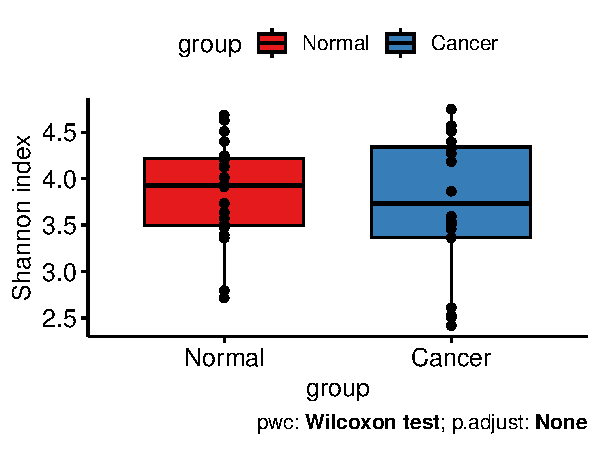
\includegraphics[width=0.7\linewidth,height=0.7\textheight]{workshop_files/figure-latex/unnamed-chunk-16-1}

\hypertarget{chao1-richness}{%
\subsubsection{Chao1 richness}\label{chao1-richness}}

\[ S = S_{obs} + \frac{F^2_1}{2F_2} \] In Chao1 estimator
\href{https://www.researchgate.net/publication/268975118_Non-parametric_estimation_of_the_classes_in_a_population}{(Chao,
A. 1984)}. \(S_{obs}\) is indicated the number of observed species,
\(F_1\) is the number of species which only once. and \(F_2\) is the
number of species which twice in community. Higher \(F_1\) indicates
that the number of non-observed species is likely to be higher. It is
expected that the community will have a relatively high abundance of
species. but \(F_2\) show the species have occurred at least twice, then
the chance of new species occurring in the community is low.

\begin{Shaded}
\begin{Highlighting}[]
\NormalTok{pwc }\OtherTok{\textless{}{-}} \FunctionTok{wilcox\_test}\NormalTok{(Chao1 }\SpecialCharTok{\textasciitilde{}}\NormalTok{ group, }\AttributeTok{paired =}\NormalTok{ F, }\AttributeTok{p.adjust.method =} \StringTok{"None"}\NormalTok{, }\AttributeTok{data =}\NormalTok{ AlphaIndex)}
\NormalTok{pwc }\OtherTok{\textless{}{-}}\NormalTok{ pwc }\SpecialCharTok{\%\textgreater{}\%} \FunctionTok{add\_xy\_position}\NormalTok{(}\AttributeTok{x =} \StringTok{"group"}\NormalTok{)}
\FunctionTok{ggboxplot}\NormalTok{(AlphaIndex, }\AttributeTok{x =} \StringTok{"group"}\NormalTok{, }\AttributeTok{y =} \StringTok{"Chao1"}\NormalTok{, }\AttributeTok{add =} \StringTok{"point"}\NormalTok{, }\AttributeTok{fill =} \StringTok{"group"}\NormalTok{) }\SpecialCharTok{+}
  \FunctionTok{scale\_fill\_brewer}\NormalTok{(}\AttributeTok{palette =} \StringTok{"Set1"}\NormalTok{) }\SpecialCharTok{+} \FunctionTok{ylab}\NormalTok{(}\StringTok{"Chao1 richness"}\NormalTok{) }\SpecialCharTok{+}
  \FunctionTok{stat\_pvalue\_manual}\NormalTok{(pwc, }\AttributeTok{hide.ns =} \ConstantTok{TRUE}\NormalTok{) }\SpecialCharTok{+}
  \FunctionTok{labs}\NormalTok{(}\AttributeTok{caption =} \FunctionTok{get\_pwc\_label}\NormalTok{(pwc))}
\end{Highlighting}
\end{Shaded}

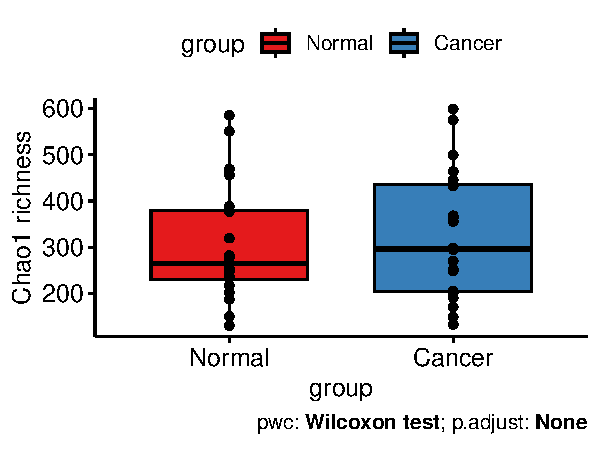
\includegraphics[width=0.7\linewidth,height=0.7\textheight]{workshop_files/figure-latex/unnamed-chunk-17-1}

\hypertarget{simpson-index}{%
\subsubsection{Simpson index}\label{simpson-index}}

\[ D_s = \sum_{i = 1}^{s} (\frac{n_i}{N})^2  \ ;\ \  D_{s^\prime    }  =  \frac{1}{D_s} \]

\href{https://www.nature.com/articles/163688a0}{Simpson (1949)} is
measure the dominance in single community. if some species is dominant
in community, the Simpson will be higher. so it can be regarded as
\texttt{concentration\ index}. In other words, the inverse Simpson index
is show the \texttt{evenness} in community.

\begin{Shaded}
\begin{Highlighting}[]
\NormalTok{pwc }\OtherTok{\textless{}{-}} \FunctionTok{wilcox\_test}\NormalTok{(Simpson }\SpecialCharTok{\textasciitilde{}}\NormalTok{ group, }\AttributeTok{paired =}\NormalTok{ F, }\AttributeTok{p.adjust.method =} \StringTok{"None"}\NormalTok{, }\AttributeTok{data =}\NormalTok{ AlphaIndex)}
\NormalTok{pwc }\OtherTok{\textless{}{-}}\NormalTok{ pwc }\SpecialCharTok{\%\textgreater{}\%} \FunctionTok{add\_xy\_position}\NormalTok{(}\AttributeTok{x =} \StringTok{"group"}\NormalTok{)}
\FunctionTok{ggboxplot}\NormalTok{(AlphaIndex, }\AttributeTok{x =} \StringTok{"group"}\NormalTok{, }\AttributeTok{y =} \StringTok{"invSimpson"}\NormalTok{, }\AttributeTok{add =} \StringTok{"point"}\NormalTok{, }\AttributeTok{fill =} \StringTok{"group"}\NormalTok{) }\SpecialCharTok{+}
  \FunctionTok{scale\_fill\_brewer}\NormalTok{(}\AttributeTok{palette =} \StringTok{"Set1"}\NormalTok{) }\SpecialCharTok{+} \FunctionTok{ylab}\NormalTok{(}\StringTok{"inverse Simpson index"}\NormalTok{) }\SpecialCharTok{+}
  \FunctionTok{stat\_pvalue\_manual}\NormalTok{(pwc, }\AttributeTok{hide.ns =} \ConstantTok{TRUE}\NormalTok{) }\SpecialCharTok{+}
  \FunctionTok{labs}\NormalTok{(}\AttributeTok{caption =} \FunctionTok{get\_pwc\_label}\NormalTok{(pwc))}
\end{Highlighting}
\end{Shaded}

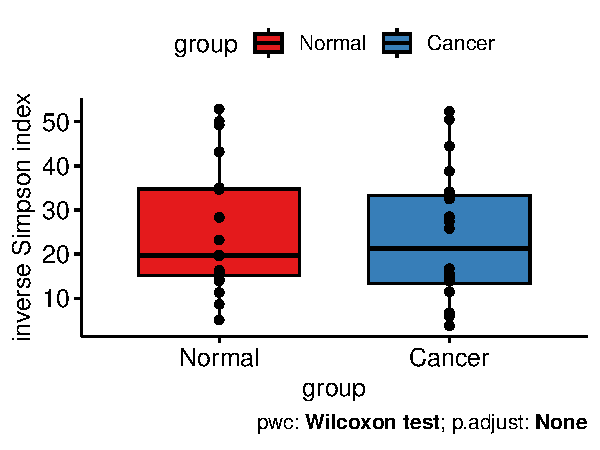
\includegraphics[width=0.7\linewidth,height=0.7\textheight]{workshop_files/figure-latex/unnamed-chunk-18-1}

\hypertarget{phylogenetic-diversity}{%
\subsubsection{Phylogenetic diversity}\label{phylogenetic-diversity}}

Faith's Phylogenetic Diversity
\href{https://www.sciencedirect.com/science/article/abs/pii/0006320792912013}{(Faith
D., 1992)} which is defined as the sum of the branch lengths of a
phylogenetic tree connecting all species, this means that PD indicates
\texttt{Feature\ diversity}.

\begin{Shaded}
\begin{Highlighting}[]
\NormalTok{pwc }\OtherTok{\textless{}{-}} \FunctionTok{wilcox\_test}\NormalTok{(PD }\SpecialCharTok{\textasciitilde{}}\NormalTok{ group, }\AttributeTok{paired =}\NormalTok{ F, }\AttributeTok{p.adjust.method =} \StringTok{"None"}\NormalTok{, }\AttributeTok{data =}\NormalTok{ AlphaIndex)}
\NormalTok{pwc }\OtherTok{\textless{}{-}}\NormalTok{ pwc }\SpecialCharTok{\%\textgreater{}\%} \FunctionTok{add\_xy\_position}\NormalTok{(}\AttributeTok{x =} \StringTok{"group"}\NormalTok{)}
\FunctionTok{ggboxplot}\NormalTok{(AlphaIndex, }\AttributeTok{x =} \StringTok{"group"}\NormalTok{, }\AttributeTok{y =} \StringTok{"PD"}\NormalTok{, }\AttributeTok{add =} \StringTok{"point"}\NormalTok{, }\AttributeTok{fill =} \StringTok{"group"}\NormalTok{) }\SpecialCharTok{+}
  \FunctionTok{scale\_fill\_brewer}\NormalTok{(}\AttributeTok{palette =} \StringTok{"Set1"}\NormalTok{) }\SpecialCharTok{+} \FunctionTok{ylab}\NormalTok{(}\StringTok{"Faith’s phylogenetic diversity"}\NormalTok{) }\SpecialCharTok{+}
  \FunctionTok{stat\_pvalue\_manual}\NormalTok{(pwc, }\AttributeTok{hide.ns =} \ConstantTok{TRUE}\NormalTok{) }\SpecialCharTok{+}
  \FunctionTok{labs}\NormalTok{(}\AttributeTok{caption =} \FunctionTok{get\_pwc\_label}\NormalTok{(pwc))}
\end{Highlighting}
\end{Shaded}

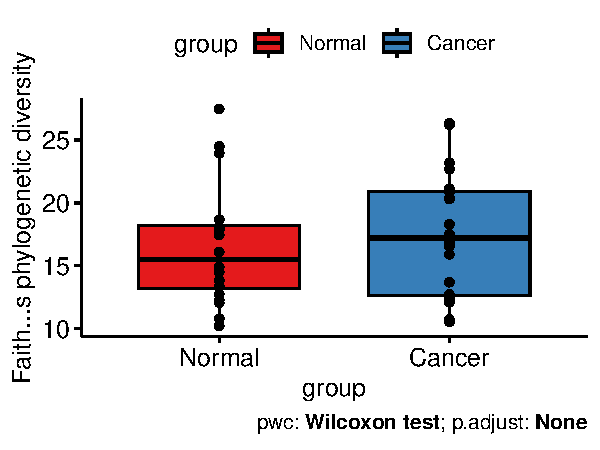
\includegraphics[width=0.7\linewidth,height=0.7\textheight]{workshop_files/figure-latex/unnamed-chunk-19-1}

\hypertarget{beta-diversity}{%
\subsection{Beta diversity}\label{beta-diversity}}

\hypertarget{bray-curtis-distance}{%
\subsubsection{Bray-Curtis distance}\label{bray-curtis-distance}}

\[ D_{BC} = \frac{\sum_{i=1}^S{|M_{i1} - M_{i2}|}}{\sum_{i=1}^S{M_{i1} + M_{i2}}} \]

In
\href{https://esajournals.onlinelibrary.wiley.com/doi/10.2307/1942268}{Bray-Curtis}
distance, \(S\) is indicates the total number of species in two
communities, \(M_{i1}\) is means the number of species \(i\) in
community 1, and so on. This method is similar to Sørensen index. and
usually utilizes non-metric multidimensional scaling
\href{https://strata.uga.edu/software/pdf/mdsTutorial.pdf}{nMDS} for
dimension reduction.

\begin{Shaded}
\begin{Highlighting}[]
\NormalTok{NMDS}\OtherTok{=}\FunctionTok{metaMDS}\NormalTok{(}\FunctionTok{t}\NormalTok{(data\_rarefied), }\AttributeTok{distance =} \StringTok{"bray"}\NormalTok{)}
\DocumentationTok{\#\# Square root transformation}
\DocumentationTok{\#\# Wisconsin double standardization}
\DocumentationTok{\#\# Run 0 stress 0.149106 }
\DocumentationTok{\#\# Run 1 stress 0.1503017 }
\DocumentationTok{\#\# Run 2 stress 0.1491056 }
\DocumentationTok{\#\# ... New best solution}
\DocumentationTok{\#\# ... Procrustes: rmse 0.0005981917  max resid 0.002768234 }
\DocumentationTok{\#\# ... Similar to previous best}
\DocumentationTok{\#\# Run 3 stress 0.1491057 }
\DocumentationTok{\#\# ... Procrustes: rmse 1.548925e{-}05  max resid 7.090235e{-}05 }
\DocumentationTok{\#\# ... Similar to previous best}
\DocumentationTok{\#\# Run 4 stress 0.1503017 }
\DocumentationTok{\#\# Run 5 stress 0.1491056 }
\DocumentationTok{\#\# ... New best solution}
\DocumentationTok{\#\# ... Procrustes: rmse 4.216836e{-}05  max resid 0.0001434376 }
\DocumentationTok{\#\# ... Similar to previous best}
\DocumentationTok{\#\# Run 6 stress 0.1491057 }
\DocumentationTok{\#\# ... Procrustes: rmse 0.0001441396  max resid 0.0005599521 }
\DocumentationTok{\#\# ... Similar to previous best}
\DocumentationTok{\#\# Run 7 stress 0.1912499 }
\DocumentationTok{\#\# Run 8 stress 0.1491055 }
\DocumentationTok{\#\# ... New best solution}
\DocumentationTok{\#\# ... Procrustes: rmse 0.0002371133  max resid 0.001049122 }
\DocumentationTok{\#\# ... Similar to previous best}
\DocumentationTok{\#\# Run 9 stress 0.1503017 }
\DocumentationTok{\#\# Run 10 stress 0.1503017 }
\DocumentationTok{\#\# Run 11 stress 0.1503084 }
\DocumentationTok{\#\# Run 12 stress 0.1491058 }
\DocumentationTok{\#\# ... Procrustes: rmse 0.0001865112  max resid 0.0008890889 }
\DocumentationTok{\#\# ... Similar to previous best}
\DocumentationTok{\#\# Run 13 stress 0.1503084 }
\DocumentationTok{\#\# Run 14 stress 0.1491059 }
\DocumentationTok{\#\# ... Procrustes: rmse 0.0002518848  max resid 0.001206103 }
\DocumentationTok{\#\# ... Similar to previous best}
\DocumentationTok{\#\# Run 15 stress 0.1503017 }
\DocumentationTok{\#\# Run 16 stress 0.1491055 }
\DocumentationTok{\#\# ... Procrustes: rmse 0.0001621694  max resid 0.0007371812 }
\DocumentationTok{\#\# ... Similar to previous best}
\DocumentationTok{\#\# Run 17 stress 0.2091891 }
\DocumentationTok{\#\# Run 18 stress 0.1503017 }
\DocumentationTok{\#\# Run 19 stress 0.1491058 }
\DocumentationTok{\#\# ... Procrustes: rmse 0.0002246621  max resid 0.00102273 }
\DocumentationTok{\#\# ... Similar to previous best}
\DocumentationTok{\#\# Run 20 stress 0.1503017 }
\DocumentationTok{\#\# *** Best solution repeated 5 times}
\NormalTok{NMDSplot }\OtherTok{\textless{}{-}} \FunctionTok{as.data.frame}\NormalTok{(NMDS}\SpecialCharTok{$}\NormalTok{points)}
\NormalTok{NMDSplot}\SpecialCharTok{$}\NormalTok{group }\OtherTok{\textless{}{-}}\NormalTok{ meta}\SpecialCharTok{$}\NormalTok{Class}
\NormalTok{prop }\OtherTok{\textless{}{-}} \FunctionTok{cmdscale}\NormalTok{(}\FunctionTok{vegdist}\NormalTok{(}\FunctionTok{t}\NormalTok{(data\_rarefied), }\AttributeTok{method =} \StringTok{"bray"}\NormalTok{), }\AttributeTok{k =} \DecValTok{2}\NormalTok{, }\AttributeTok{eig =}\NormalTok{ T, }\AttributeTok{add =}\NormalTok{ T )}
\NormalTok{prop }\OtherTok{\textless{}{-}} \FunctionTok{round}\NormalTok{(prop}\SpecialCharTok{$}\NormalTok{eig}\SpecialCharTok{*}\DecValTok{100}\SpecialCharTok{/}\FunctionTok{sum}\NormalTok{(prop}\SpecialCharTok{$}\NormalTok{eig),}\DecValTok{1}\NormalTok{)}
\FunctionTok{print}\NormalTok{(prop[}\DecValTok{1}\SpecialCharTok{:}\DecValTok{8}\NormalTok{]) }\CommentTok{\# chick the proportion of variance explained}
\DocumentationTok{\#\# [1] 11.7  9.9  7.6  5.7  5.4  4.5  3.8  3.7}
\FunctionTok{stressplot}\NormalTok{(NMDS) }\CommentTok{\# chick the fitness in nMDS}
\end{Highlighting}
\end{Shaded}

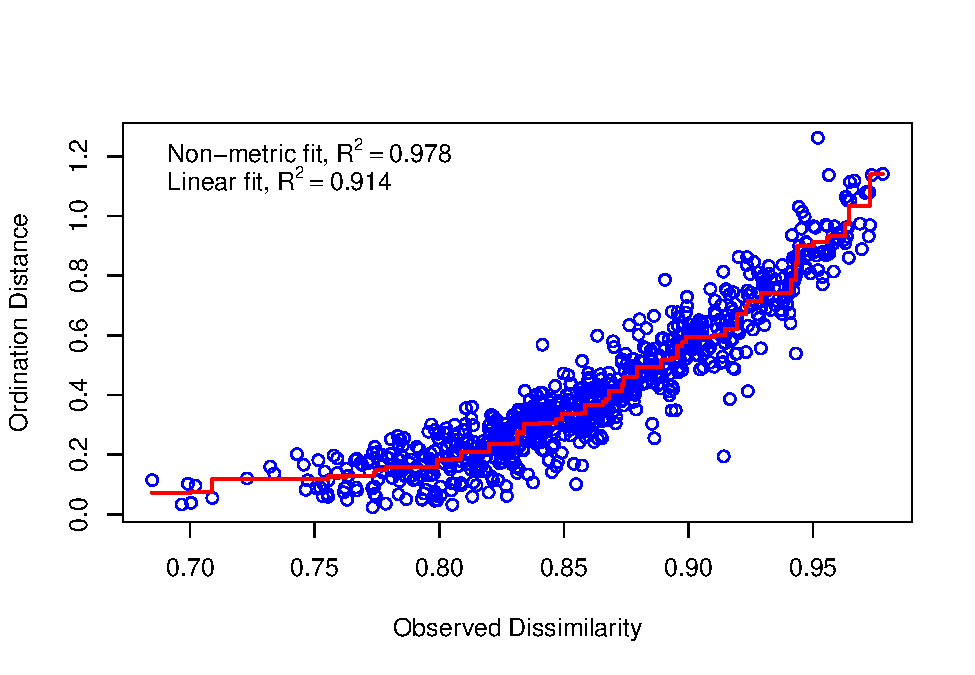
\includegraphics[width=0.7\linewidth,height=0.7\textheight]{workshop_files/figure-latex/unnamed-chunk-20-1}

\begin{Shaded}
\begin{Highlighting}[]
\FunctionTok{ggscatter}\NormalTok{(NMDSplot, }\AttributeTok{x =} \StringTok{"MDS1"}\NormalTok{, }\AttributeTok{y =} \StringTok{"MDS2"}\NormalTok{,}\AttributeTok{combine  =}\NormalTok{ T, }\AttributeTok{color =} \StringTok{\textquotesingle{}group\textquotesingle{}}\NormalTok{,}
          \AttributeTok{ellipse.type =} \StringTok{"norm"}\NormalTok{, }\AttributeTok{ellipse =}\NormalTok{ T,}\AttributeTok{ellipse.level =} \FloatTok{0.5}\NormalTok{, }\AttributeTok{ellipse.alpha =} \FloatTok{0.5}\NormalTok{, }\AttributeTok{repel =} \ConstantTok{TRUE}\NormalTok{) }\SpecialCharTok{+}
          \FunctionTok{scale\_color\_manual}\NormalTok{(}\AttributeTok{values =} \FunctionTok{c}\NormalTok{(}\StringTok{"\#CC0000"}\NormalTok{,}\StringTok{"\#FFAA33"}\NormalTok{))}\SpecialCharTok{+}
          \FunctionTok{scale\_fill\_manual}\NormalTok{(}\AttributeTok{values =} \FunctionTok{c}\NormalTok{(}\StringTok{"\#CC0000"}\NormalTok{,}\StringTok{"\#FFAA33"}\NormalTok{)) }\SpecialCharTok{+}
          \FunctionTok{xlab}\NormalTok{(}\FunctionTok{paste0}\NormalTok{(}\FunctionTok{c}\NormalTok{(}\StringTok{\textquotesingle{}PC1 (\textquotesingle{}}\NormalTok{, prop[}\DecValTok{1}\NormalTok{],}\StringTok{\textquotesingle{}\% var.explained)\textquotesingle{}}\NormalTok{), }\AttributeTok{collapse =} \StringTok{""}\NormalTok{)) }\SpecialCharTok{+} 
          \FunctionTok{ylab}\NormalTok{(}\FunctionTok{paste0}\NormalTok{(}\FunctionTok{c}\NormalTok{(}\StringTok{\textquotesingle{}PC1 (\textquotesingle{}}\NormalTok{, prop[}\DecValTok{2}\NormalTok{],}\StringTok{\textquotesingle{}\% var.explained)\textquotesingle{}}\NormalTok{), }\AttributeTok{collapse =} \StringTok{""}\NormalTok{)) }\SpecialCharTok{+}
          \FunctionTok{theme}\NormalTok{(}\AttributeTok{panel.background =} \FunctionTok{element\_rect}\NormalTok{(}\AttributeTok{fill =} \StringTok{\textquotesingle{}transparent\textquotesingle{}}\NormalTok{),}
                \AttributeTok{panel.grid =} \FunctionTok{element\_blank}\NormalTok{(),}
                \AttributeTok{axis.ticks.length =} \FunctionTok{unit}\NormalTok{(}\FloatTok{0.4}\NormalTok{,}\StringTok{"lines"}\NormalTok{),}
                \AttributeTok{axis.ticks =} \FunctionTok{element\_line}\NormalTok{(}\AttributeTok{color=}\StringTok{\textquotesingle{}black\textquotesingle{}}\NormalTok{),}
                \AttributeTok{axis.line =} \FunctionTok{element\_line}\NormalTok{(}\AttributeTok{colour =} \StringTok{"black"}\NormalTok{),}
                \AttributeTok{legend.title=}\FunctionTok{element\_blank}\NormalTok{(),}
                \AttributeTok{legend.position  =} \StringTok{\textquotesingle{}right\textquotesingle{}}\NormalTok{)}
\end{Highlighting}
\end{Shaded}

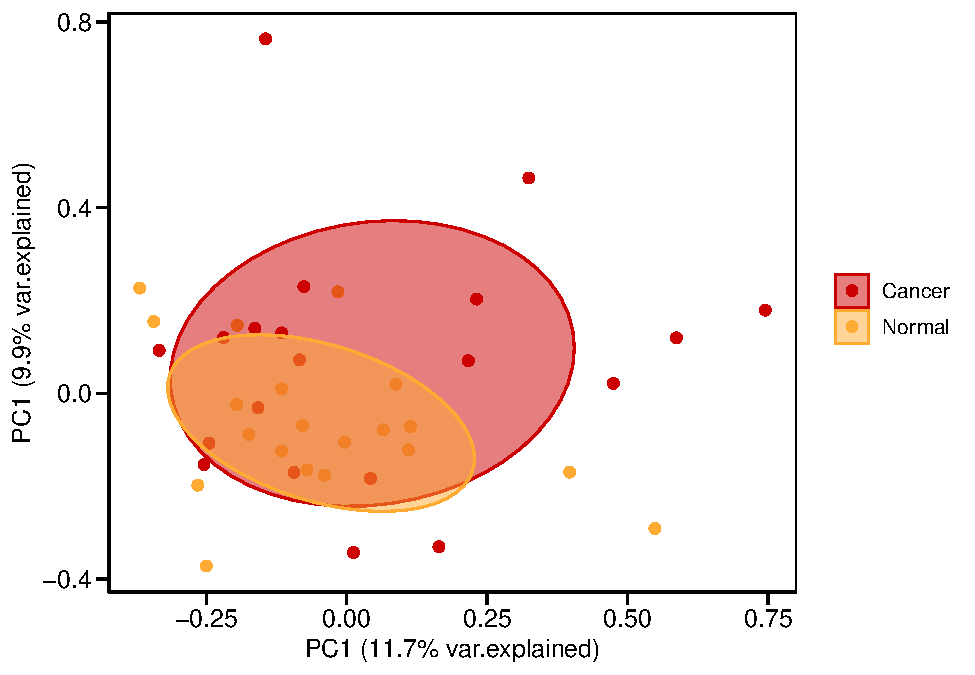
\includegraphics[width=0.7\linewidth,height=0.7\textheight]{workshop_files/figure-latex/unnamed-chunk-20-2}

Ellipse type can choose the \texttt{convex}, \texttt{confidence},
\texttt{t}, \texttt{euclid}.

\hypertarget{unifrac-distance}{%
\subsubsection{Unifrac distance}\label{unifrac-distance}}

\begin{itemize}
\item
  unWeighted
  \[ U_{uw} = \frac{\sum_{i=1}^N{l_i|A_{i} - B_{i}|}}{\sum_{i=1}^N{ max(A_{i} + B_{i})}} \]
\item
  Weighted
  \[ U_{w} = \frac{\sum_{i=1}^n{b_i| \frac{A_{i}}{A_T} - \frac{B_{i}}{B_T}|}}{\sum_{j=1}^S{L_j}} \]
\end{itemize}

\begin{Shaded}
\begin{Highlighting}[]
\NormalTok{ASV }\OtherTok{=} \FunctionTok{otu\_table}\NormalTok{(data\_rarefied, }\AttributeTok{taxa\_are\_rows =} \ConstantTok{TRUE}\NormalTok{)}
\NormalTok{TAX }\OtherTok{=} \FunctionTok{tax\_table}\NormalTok{(}\FunctionTok{as.matrix}\NormalTok{(taxa))}
\NormalTok{physeq }\OtherTok{=} \FunctionTok{phyloseq}\NormalTok{(ASV, TAX, tree)}
\NormalTok{Unif }\OtherTok{=} \FunctionTok{UniFrac}\NormalTok{(physeq, }\AttributeTok{weighted =}\NormalTok{ F, }\AttributeTok{normalized =}\NormalTok{ F, }\AttributeTok{parallel =}\NormalTok{ F)  }\CommentTok{\# if weighted = TRUE; then weighted UniFrac}
\NormalTok{Unif\_d }\OtherTok{\textless{}{-}} \FunctionTok{pcoa}\NormalTok{(Unif)}
\NormalTok{Unifplot }\OtherTok{\textless{}{-}} \FunctionTok{data.frame}\NormalTok{(}\AttributeTok{axis1 =} \FunctionTok{as.numeric}\NormalTok{(Unif\_d}\SpecialCharTok{$}\NormalTok{vectors[,}\DecValTok{1}\NormalTok{]),}
                       \AttributeTok{axis2 =} \FunctionTok{as.numeric}\NormalTok{(Unif\_d}\SpecialCharTok{$}\NormalTok{vectors[,}\DecValTok{2}\NormalTok{]))}
\NormalTok{Unifplot}\SpecialCharTok{$}\NormalTok{group }\OtherTok{\textless{}{-}}\NormalTok{ meta}\SpecialCharTok{$}\NormalTok{Class}
\NormalTok{prop }\OtherTok{\textless{}{-}} \FunctionTok{cmdscale}\NormalTok{(Unif, }\AttributeTok{k =} \DecValTok{2}\NormalTok{, }\AttributeTok{eig =}\NormalTok{ T, }\AttributeTok{add =}\NormalTok{ T)}
\NormalTok{prop }\OtherTok{\textless{}{-}} \FunctionTok{round}\NormalTok{(prop}\SpecialCharTok{$}\NormalTok{eig}\SpecialCharTok{*}\DecValTok{100}\SpecialCharTok{/}\FunctionTok{sum}\NormalTok{(prop}\SpecialCharTok{$}\NormalTok{eig),}\DecValTok{1}\NormalTok{)}
\FunctionTok{print}\NormalTok{(prop[}\DecValTok{1}\SpecialCharTok{:}\DecValTok{8}\NormalTok{]) }\CommentTok{\# chick the proportion of variance explained}
\DocumentationTok{\#\# [1] 15.0  7.9  6.3  4.0  3.7  3.4  3.3  3.2}

\FunctionTok{ggscatter}\NormalTok{(Unifplot, }\AttributeTok{x =} \StringTok{"axis1"}\NormalTok{, }\AttributeTok{y =} \StringTok{"axis2"}\NormalTok{,}\AttributeTok{combine =}\NormalTok{ T, }\AttributeTok{color =} \StringTok{\textquotesingle{}group\textquotesingle{}}\NormalTok{,}
          \AttributeTok{ellipse.type =} \StringTok{"norm"}\NormalTok{, }\AttributeTok{ellipse =}\NormalTok{ T,}\AttributeTok{ellipse.level =} \FloatTok{0.5}\NormalTok{, }\AttributeTok{ellipse.alpha =} \FloatTok{0.5}\NormalTok{, }\AttributeTok{repel =} \ConstantTok{TRUE}\NormalTok{) }\SpecialCharTok{+}
          \FunctionTok{scale\_color\_manual}\NormalTok{(}\AttributeTok{values =} \FunctionTok{c}\NormalTok{(}\StringTok{"\#CC0000"}\NormalTok{,}\StringTok{"\#FFAA33"}\NormalTok{))}\SpecialCharTok{+}
          \FunctionTok{scale\_fill\_manual}\NormalTok{(}\AttributeTok{values =} \FunctionTok{c}\NormalTok{(}\StringTok{"\#CC0000"}\NormalTok{,}\StringTok{"\#FFAA33"}\NormalTok{)) }\SpecialCharTok{+}
          \FunctionTok{xlab}\NormalTok{(}\FunctionTok{paste0}\NormalTok{(}\FunctionTok{c}\NormalTok{(}\StringTok{\textquotesingle{}PCoA1 (\textquotesingle{}}\NormalTok{, prop[}\DecValTok{1}\NormalTok{],}\StringTok{\textquotesingle{}\% var.explained)\textquotesingle{}}\NormalTok{), }\AttributeTok{collapse =} \StringTok{""}\NormalTok{)) }\SpecialCharTok{+} 
          \FunctionTok{ylab}\NormalTok{(}\FunctionTok{paste0}\NormalTok{(}\FunctionTok{c}\NormalTok{(}\StringTok{\textquotesingle{}PCoA1 (\textquotesingle{}}\NormalTok{, prop[}\DecValTok{2}\NormalTok{],}\StringTok{\textquotesingle{}\% var.explained)\textquotesingle{}}\NormalTok{), }\AttributeTok{collapse =} \StringTok{""}\NormalTok{)) }\SpecialCharTok{+}
          \FunctionTok{theme}\NormalTok{(}\AttributeTok{panel.background =} \FunctionTok{element\_rect}\NormalTok{(}\AttributeTok{fill =} \StringTok{\textquotesingle{}transparent\textquotesingle{}}\NormalTok{),}
                \AttributeTok{panel.grid =} \FunctionTok{element\_blank}\NormalTok{(),}
                \AttributeTok{axis.ticks.length =} \FunctionTok{unit}\NormalTok{(}\FloatTok{0.4}\NormalTok{,}\StringTok{"lines"}\NormalTok{),}
                \AttributeTok{axis.ticks =} \FunctionTok{element\_line}\NormalTok{(}\AttributeTok{color=}\StringTok{\textquotesingle{}black\textquotesingle{}}\NormalTok{),}
                \AttributeTok{axis.line =} \FunctionTok{element\_line}\NormalTok{(}\AttributeTok{colour =} \StringTok{"black"}\NormalTok{),}
                \AttributeTok{legend.title=}\FunctionTok{element\_blank}\NormalTok{(),}
                \AttributeTok{legend.position  =} \StringTok{\textquotesingle{}right\textquotesingle{}}\NormalTok{)}
\end{Highlighting}
\end{Shaded}

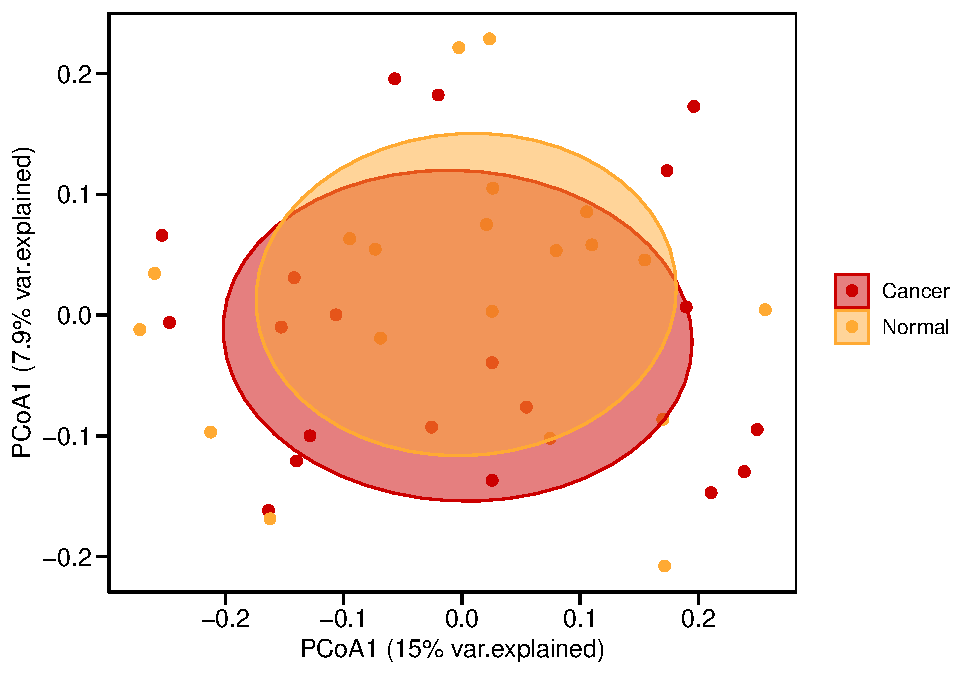
\includegraphics[width=0.7\linewidth,height=0.7\textheight]{workshop_files/figure-latex/unnamed-chunk-21-1}

\hypertarget{anosim}{%
\subsubsection{ANOSIM}\label{anosim}}

Analysis of similarities \texttt{(ANOSIM)} is a non-parametric
statistical test widely used in the field of ecology. As an ANOVA-like
test, where instead of operating on raw data, operates on a ranked
dissimilarity matrix.

Given a matrix of rank dissimilarities between a set of samples, each
solely belong to one treatment group, the ANOSIM tests whether we can
reject the null hypothesis that the similarity between groups is greater
than or equal to the similarity within the groups.

The test statistic R is calculated in the following way:

\[ R={\frac {\bar{r_{B}}-\bar{r_{W}}}{M/2}} \]

where \(\bar{r_{B}}\) is the average of rank similarities of pairs of
samples (or replicates) originating from different sites, \(\bar{r_W}\)
is the average of rank similarity of pairs among replicates within
sites, and \(M\) = n(n − 1)/2 where n is the number of samples.

\begin{Shaded}
\begin{Highlighting}[]
\FunctionTok{anosim}\NormalTok{(}\FunctionTok{vegdist}\NormalTok{(}\FunctionTok{t}\NormalTok{(data\_rarefied), }\AttributeTok{method =} \StringTok{"bray"}\NormalTok{), meta}\SpecialCharTok{$}\NormalTok{Class)}
\DocumentationTok{\#\# }
\DocumentationTok{\#\# Call:}
\DocumentationTok{\#\# anosim(x = vegdist(t(data\_rarefied), method = "bray"), grouping = meta$Class) }
\DocumentationTok{\#\# Dissimilarity: bray }
\DocumentationTok{\#\# }
\DocumentationTok{\#\# ANOSIM statistic R: 0.08716 }
\DocumentationTok{\#\#       Significance: 0.004 }
\DocumentationTok{\#\# }
\DocumentationTok{\#\# Permutation: free}
\DocumentationTok{\#\# Number of permutations: 999}
\FunctionTok{anosim}\NormalTok{(Unif, meta}\SpecialCharTok{$}\NormalTok{Class)}
\DocumentationTok{\#\# }
\DocumentationTok{\#\# Call:}
\DocumentationTok{\#\# anosim(x = Unif, grouping = meta$Class) }
\DocumentationTok{\#\# Dissimilarity: }
\DocumentationTok{\#\# }
\DocumentationTok{\#\# ANOSIM statistic R: 0.01125 }
\DocumentationTok{\#\#       Significance: 0.274 }
\DocumentationTok{\#\# }
\DocumentationTok{\#\# Permutation: free}
\DocumentationTok{\#\# Number of permutations: 999}
\end{Highlighting}
\end{Shaded}

\hypertarget{adonis2}{%
\subsubsection{adonis2}\label{adonis2}}

Permutational Multivariate Analysis of Variance \texttt{(adonis)},

\begin{Shaded}
\begin{Highlighting}[]
\FunctionTok{adonis2}\NormalTok{(}\FunctionTok{t}\NormalTok{(data\_rarefied) }\SpecialCharTok{\textasciitilde{}}\NormalTok{ Class, }\AttributeTok{data =}\NormalTok{ meta, }\AttributeTok{method=} \StringTok{"bray"}\NormalTok{)}
\DocumentationTok{\#\# Permutation test for adonis under reduced model}
\DocumentationTok{\#\# Terms added sequentially (first to last)}
\DocumentationTok{\#\# Permutation: free}
\DocumentationTok{\#\# Number of permutations: 999}
\DocumentationTok{\#\# }
\DocumentationTok{\#\# adonis2(formula = t(data\_rarefied) \textasciitilde{} Class, data = meta, method = "bray")}
\DocumentationTok{\#\#          Df SumOfSqs      R2    F Pr(\textgreater{}F)  }
\DocumentationTok{\#\# Class     1   0.5381 0.04186 1.66  0.015 *}
\DocumentationTok{\#\# Residual 38  12.3178 0.95814              }
\DocumentationTok{\#\# Total    39  12.8559 1.00000              }
\DocumentationTok{\#\# {-}{-}{-}}
\DocumentationTok{\#\# Signif. codes:  0 \textquotesingle{}***\textquotesingle{} 0.001 \textquotesingle{}**\textquotesingle{} 0.01 \textquotesingle{}*\textquotesingle{} 0.05 \textquotesingle{}.\textquotesingle{} 0.1 \textquotesingle{} \textquotesingle{} 1}
\FunctionTok{adonis2}\NormalTok{(Unif }\SpecialCharTok{\textasciitilde{}}\NormalTok{ Class, }\AttributeTok{data =}\NormalTok{ meta)}
\DocumentationTok{\#\# Permutation test for adonis under reduced model}
\DocumentationTok{\#\# Terms added sequentially (first to last)}
\DocumentationTok{\#\# Permutation: free}
\DocumentationTok{\#\# Number of permutations: 999}
\DocumentationTok{\#\# }
\DocumentationTok{\#\# adonis2(formula = Unif \textasciitilde{} Class, data = meta)}
\DocumentationTok{\#\#          Df SumOfSqs      R2      F Pr(\textgreater{}F)}
\DocumentationTok{\#\# Class     1   0.1782 0.02849 1.1142  0.244}
\DocumentationTok{\#\# Residual 38   6.0787 0.97151              }
\DocumentationTok{\#\# Total    39   6.2569 1.00000}
\end{Highlighting}
\end{Shaded}

\hypertarget{community-composition}{%
\subsection{Community composition}\label{community-composition}}

sort by major species decrease

\begin{Shaded}
\begin{Highlighting}[]
\CommentTok{\# choose the taxonomic rank for visualization}
\FunctionTok{print}\NormalTok{(}\FunctionTok{colnames}\NormalTok{(taxa))}
\DocumentationTok{\#\# [1] "Kingdom" "Phylum"  "Class"   "Order"   "Family"  "Genus"   "Species"}
\CommentTok{\# get\_composition function is sourced from utils.R}
\NormalTok{compair }\OtherTok{\textless{}{-}} \FunctionTok{get\_composition}\NormalTok{(data, taxa, }\StringTok{\textquotesingle{}Order\textquotesingle{}}\NormalTok{, meta, }\StringTok{\textquotesingle{}Class\textquotesingle{}}\NormalTok{)}

\FunctionTok{ggplot}\NormalTok{(compair, }\FunctionTok{aes}\NormalTok{(}\AttributeTok{x =}\NormalTok{ sample, }\AttributeTok{y =}\NormalTok{ percentage, }\AttributeTok{fill =}\NormalTok{ taxa)) }\SpecialCharTok{+} 
  \FunctionTok{geom\_bar}\NormalTok{(}\AttributeTok{stat=}\StringTok{"identity"}\NormalTok{,}\AttributeTok{colour =} \StringTok{"black"}\NormalTok{) }\SpecialCharTok{+} \FunctionTok{scale\_fill\_brewer}\NormalTok{(}\AttributeTok{palette =} \StringTok{"Paired"}\NormalTok{) }\SpecialCharTok{+}
  \FunctionTok{labs}\NormalTok{(}\AttributeTok{fill =} \StringTok{"Order"}\NormalTok{) }\SpecialCharTok{+} \FunctionTok{ylab}\NormalTok{(}\StringTok{"Relative abundance (\%)"}\NormalTok{) }\SpecialCharTok{+} 
  \CommentTok{\#facet\_grid(\textasciitilde{}group, space="free", scales="free") + \# separate the group}
  \FunctionTok{theme}\NormalTok{(}\AttributeTok{axis.text.x =} \FunctionTok{element\_blank}\NormalTok{(),}
        \AttributeTok{axis.line =} \FunctionTok{element\_line}\NormalTok{(}\AttributeTok{linetype =} \DecValTok{1}\NormalTok{,}\AttributeTok{colour =} \StringTok{\textquotesingle{}black\textquotesingle{}}\NormalTok{),}
        \AttributeTok{panel.background =} \FunctionTok{element\_rect}\NormalTok{(}\FunctionTok{I}\NormalTok{(}\DecValTok{0}\NormalTok{)),}
        \AttributeTok{panel.grid.major =} \FunctionTok{element\_line}\NormalTok{(}\AttributeTok{colour =} \ConstantTok{NA}\NormalTok{),}
        \AttributeTok{panel.grid.minor =} \FunctionTok{element\_line}\NormalTok{(}\AttributeTok{colour =} \ConstantTok{NA}\NormalTok{),}
        \AttributeTok{text =} \FunctionTok{element\_text}\NormalTok{(}\AttributeTok{size=}\DecValTok{16}\NormalTok{))}
\end{Highlighting}
\end{Shaded}

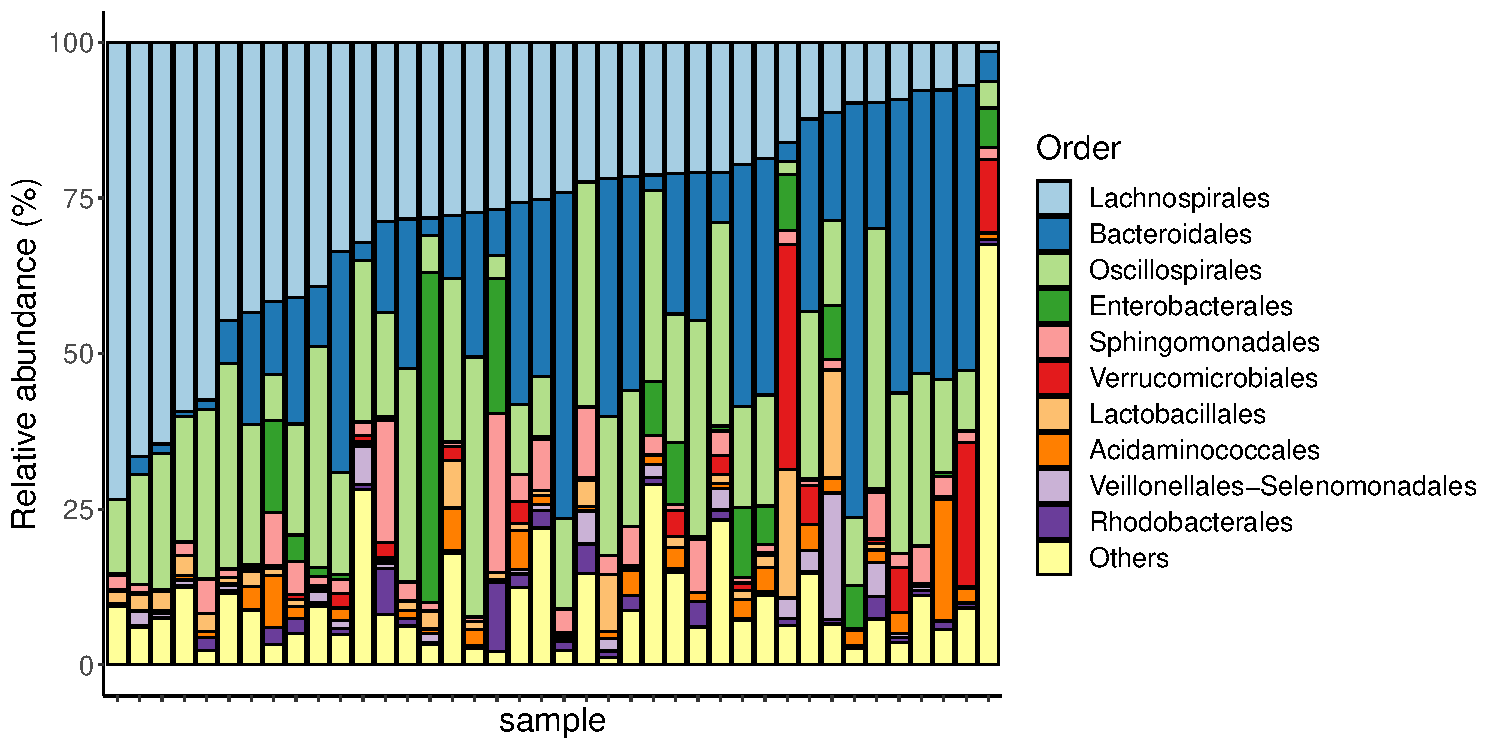
\includegraphics{workshop_files/figure-latex/unnamed-chunk-24-1.pdf}

sort by hierarchical clustering

\begin{Shaded}
\begin{Highlighting}[]
\NormalTok{compair\_2D }\OtherTok{\textless{}{-}} \FunctionTok{reshape}\NormalTok{(compair[,}\DecValTok{1}\SpecialCharTok{:}\DecValTok{3}\NormalTok{], }\AttributeTok{idvar =} \StringTok{"sample"}\NormalTok{, }\AttributeTok{timevar =} \StringTok{"taxa"}\NormalTok{, }\AttributeTok{direction =} \StringTok{"wide"}\NormalTok{)}
\FunctionTok{rownames}\NormalTok{(compair\_2D) }\OtherTok{\textless{}{-}}\NormalTok{ compair\_2D[,}\DecValTok{1}\NormalTok{]}
\NormalTok{compair\_2D }\OtherTok{\textless{}{-}}\NormalTok{ compair\_2D[,}\DecValTok{2}\SpecialCharTok{:}\FunctionTok{ncol}\NormalTok{(compair\_2D)]}
\NormalTok{horder }\OtherTok{\textless{}{-}} \FunctionTok{hclust}\NormalTok{(}\FunctionTok{dist}\NormalTok{(compair\_2D), }\AttributeTok{method =} \StringTok{\textquotesingle{}ward.D\textquotesingle{}}\NormalTok{)}
\NormalTok{horder }\OtherTok{\textless{}{-}}\NormalTok{ horder}\SpecialCharTok{$}\NormalTok{labels[horder}\SpecialCharTok{$}\NormalTok{order]}
\NormalTok{compair}\SpecialCharTok{$}\NormalTok{sample }\OtherTok{\textless{}{-}} \FunctionTok{factor}\NormalTok{(compair}\SpecialCharTok{$}\NormalTok{sample, }\AttributeTok{levels =}\NormalTok{ horder)}

\FunctionTok{ggplot}\NormalTok{(compair, }\FunctionTok{aes}\NormalTok{(}\AttributeTok{x =}\NormalTok{ sample, }\AttributeTok{y =}\NormalTok{ percentage, }\AttributeTok{fill =}\NormalTok{ taxa)) }\SpecialCharTok{+} 
  \FunctionTok{geom\_bar}\NormalTok{(}\AttributeTok{stat=}\StringTok{"identity"}\NormalTok{,}\AttributeTok{colour =} \StringTok{"black"}\NormalTok{) }\SpecialCharTok{+} \FunctionTok{scale\_fill\_brewer}\NormalTok{(}\AttributeTok{palette =} \StringTok{"Paired"}\NormalTok{) }\SpecialCharTok{+}
  \FunctionTok{labs}\NormalTok{(}\AttributeTok{fill =} \StringTok{"Order"}\NormalTok{) }\SpecialCharTok{+} \FunctionTok{ylab}\NormalTok{(}\StringTok{"Relative abundance (\%)"}\NormalTok{) }\SpecialCharTok{+} 
  \CommentTok{\#facet\_grid(\textasciitilde{}group, space="free", scales="free") + \# separate the group}
  \FunctionTok{theme}\NormalTok{(}\AttributeTok{axis.text.x =} \FunctionTok{element\_blank}\NormalTok{(),}
        \AttributeTok{axis.line =} \FunctionTok{element\_line}\NormalTok{(}\AttributeTok{linetype =} \DecValTok{1}\NormalTok{,}\AttributeTok{colour =} \StringTok{\textquotesingle{}black\textquotesingle{}}\NormalTok{),}
        \AttributeTok{panel.background =} \FunctionTok{element\_rect}\NormalTok{(}\FunctionTok{I}\NormalTok{(}\DecValTok{0}\NormalTok{)),}
        \AttributeTok{panel.grid.major =} \FunctionTok{element\_line}\NormalTok{(}\AttributeTok{colour =} \ConstantTok{NA}\NormalTok{),}
        \AttributeTok{panel.grid.minor =} \FunctionTok{element\_line}\NormalTok{(}\AttributeTok{colour =} \ConstantTok{NA}\NormalTok{),}
        \AttributeTok{text =} \FunctionTok{element\_text}\NormalTok{(}\AttributeTok{size=}\DecValTok{16}\NormalTok{))}
\end{Highlighting}
\end{Shaded}

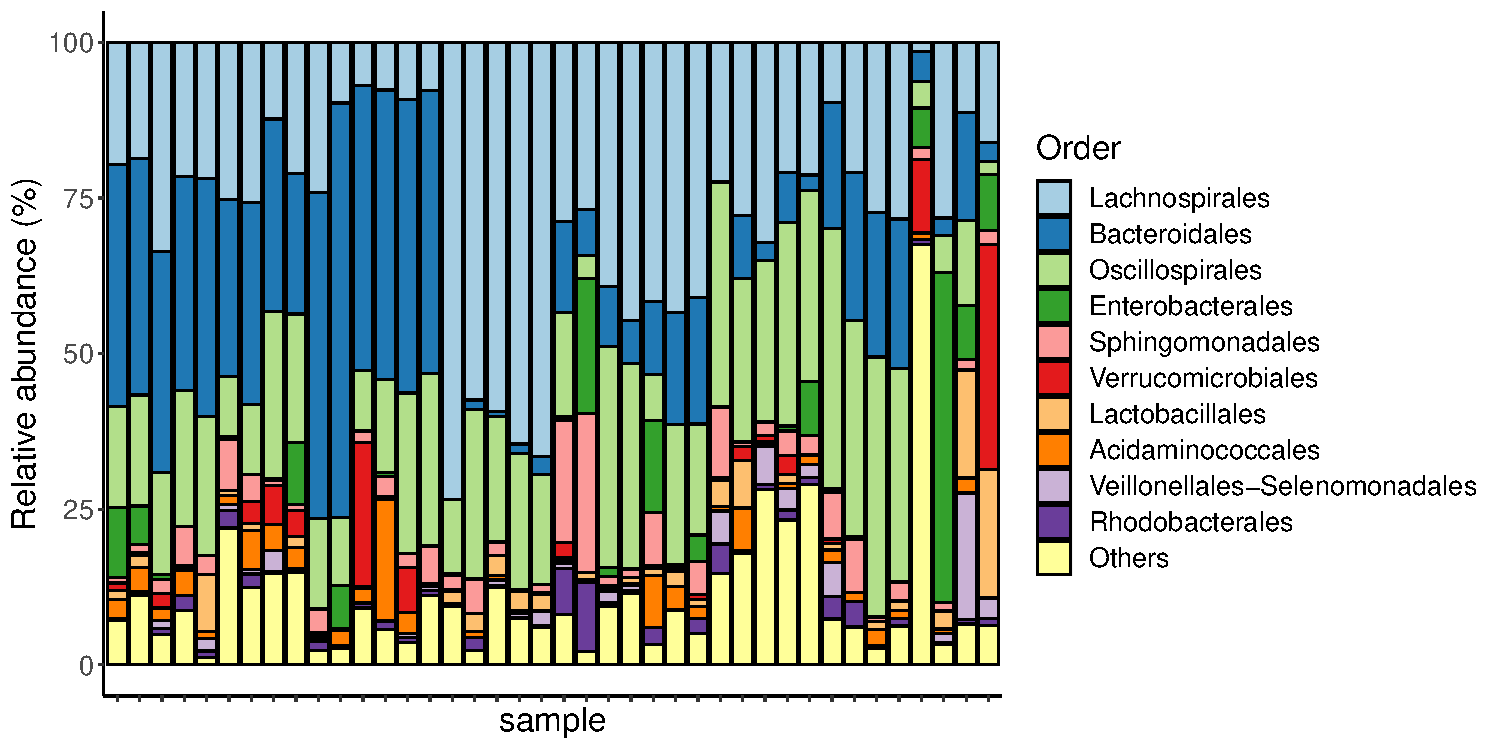
\includegraphics{workshop_files/figure-latex/unnamed-chunk-25-1.pdf}

\hypertarget{environmental-analysis}{%
\section{Environmental Analysis}\label{environmental-analysis}}

To demonstrate how the environmental factor impacting in microbiota, we
use wetland microbiota which characterised by ions concentration. the
soil samples were collected from 4 wetland in southern Taiwan and named
as AA, BB, CC, DD respectively. and each sample had be measured with
LCMS.

\begin{Shaded}
\begin{Highlighting}[]
\NormalTok{wetland }\OtherTok{\textless{}{-}} \FunctionTok{read.table}\NormalTok{(}\StringTok{"\textasciitilde{}/Course/NDMC\_2025/data/wetland/ASV\_table.txt"}\NormalTok{, }\AttributeTok{sep =} \StringTok{"}\SpecialCharTok{\textbackslash{}t}\StringTok{"}\NormalTok{, }\AttributeTok{stringsAsFactors =}\NormalTok{ F)}
\NormalTok{ion }\OtherTok{\textless{}{-}} \FunctionTok{read.table}\NormalTok{(}\StringTok{"\textasciitilde{}/Course/NDMC\_2025/data/wetland/ion.txt"}\NormalTok{, }\AttributeTok{sep =} \StringTok{"}\SpecialCharTok{\textbackslash{}t}\StringTok{"}\NormalTok{, }\AttributeTok{stringsAsFactors =}\NormalTok{ F)}
\NormalTok{wetland }\OtherTok{\textless{}{-}}\NormalTok{ wetland[,}\FunctionTok{rownames}\NormalTok{(ion)]}
\FunctionTok{head}\NormalTok{(wetland[,}\DecValTok{1}\SpecialCharTok{:}\DecValTok{5}\NormalTok{])}
\DocumentationTok{\#\#                AA1 AA2 AA3 AA4  AA5}
\DocumentationTok{\#\# ASV\_V3V400009    0 196   0  13    7}
\DocumentationTok{\#\# ASV\_V3V400024    0   0   0   0    0}
\DocumentationTok{\#\# ASV\_V3V400036 2846  26 552   0 2030}
\DocumentationTok{\#\# ASV\_V3V400040    0   0   0   0    0}
\DocumentationTok{\#\# ASV\_V3V400042  821 793 947 633  427}
\DocumentationTok{\#\# ASV\_V3V400043    0   0   0   3    0}
\FunctionTok{head}\NormalTok{(ion)}
\DocumentationTok{\#\#          Na      K      Mg      Ca      Cl    Br    SO4     EC    pH  Salinity}
\DocumentationTok{\#\# AA1   538.0  45.76   93.40   78.33   775.3   0.0  321.9   3600 7.143  1.610759}
\DocumentationTok{\#\# AA2   691.1  47.13   87.07   49.96   703.3   0.0  164.2   4020 7.675  1.799610}
\DocumentationTok{\#\# AA3   716.1  56.79  124.20  151.00   920.1   0.0  418.2   4330 6.862  2.040961}
\DocumentationTok{\#\# AA4   651.2  80.48   97.89   89.33   727.9   0.0  244.4   3640 6.330  1.755768}
\DocumentationTok{\#\# AA5   576.9   0.00   85.44   83.32   748.3   0.0  326.7   3510 6.670  1.650724}
\DocumentationTok{\#\# BB1 23830.0 922.90 2989.00 1494.00 37540.0 266.6 5298.0 137700 6.701 74.292982}
\end{Highlighting}
\end{Shaded}

\hypertarget{mantel-test}{%
\subsection{Mantel test}\label{mantel-test}}

The Mantel test computes the Pearson or Spearman correlation between two
distance matrices and evaluates its significance using a permutation
test.

\begin{Shaded}
\begin{Highlighting}[]
\NormalTok{min }\OtherTok{\textless{}{-}} \FunctionTok{min}\NormalTok{(}\FunctionTok{colSums}\NormalTok{(wetland))}
\NormalTok{wetland\_rarefied }\OtherTok{\textless{}{-}} \FunctionTok{t}\NormalTok{(}\FunctionTok{rrarefy}\NormalTok{(}\FunctionTok{t}\NormalTok{(wetland), min))}
\NormalTok{wetland\_rarefied }\OtherTok{\textless{}{-}}\NormalTok{ wetland\_rarefied[}\FunctionTok{rowSums}\NormalTok{(wetland\_rarefied) }\SpecialCharTok{\textgreater{}} \DecValTok{0}\NormalTok{,]}

\NormalTok{manteldf }\OtherTok{\textless{}{-}} \FunctionTok{data.frame}\NormalTok{(}\AttributeTok{Factor =} \DecValTok{0}\NormalTok{, }\AttributeTok{rho =} \DecValTok{0}\NormalTok{, }\AttributeTok{p\_value =} \DecValTok{0}\NormalTok{)}
\NormalTok{count }\OtherTok{\textless{}{-}} \DecValTok{1}
\ControlFlowTok{for}\NormalTok{(i }\ControlFlowTok{in} \DecValTok{1}\SpecialCharTok{:}\FunctionTok{ncol}\NormalTok{(ion))\{}
\NormalTok{  Mantel\_res }\OtherTok{\textless{}{-}} \FunctionTok{mantel}\NormalTok{(}\FunctionTok{dist}\NormalTok{(ion[,i]),}\FunctionTok{vegdist}\NormalTok{(}\FunctionTok{t}\NormalTok{(wetland\_rarefied)), }\AttributeTok{method =} \StringTok{"spearman"}\NormalTok{)}
\NormalTok{  manteldf[count,}\DecValTok{1}\NormalTok{] }\OtherTok{\textless{}{-}} \FunctionTok{colnames}\NormalTok{(ion)[i]}
\NormalTok{  manteldf[count,}\DecValTok{2}\NormalTok{] }\OtherTok{\textless{}{-}} \FunctionTok{round}\NormalTok{(Mantel\_res}\SpecialCharTok{$}\NormalTok{statistic,}\DecValTok{4}\NormalTok{)}
\NormalTok{  manteldf[count,}\DecValTok{3}\NormalTok{] }\OtherTok{\textless{}{-}} \FunctionTok{round}\NormalTok{(Mantel\_res}\SpecialCharTok{$}\NormalTok{signif,}\DecValTok{4}\NormalTok{)}
\NormalTok{  count }\OtherTok{=}\NormalTok{ count }\SpecialCharTok{+} \DecValTok{1}
\NormalTok{\}}
\NormalTok{manteldf}
\DocumentationTok{\#\#      Factor    rho p\_value}
\DocumentationTok{\#\# 1        Na 0.7629   0.001}
\DocumentationTok{\#\# 2         K 0.1049   0.121}
\DocumentationTok{\#\# 3        Mg 0.6716   0.001}
\DocumentationTok{\#\# 4        Ca 0.7391   0.001}
\DocumentationTok{\#\# 5        Cl 0.7424   0.001}
\DocumentationTok{\#\# 6        Br 0.1665   0.033}
\DocumentationTok{\#\# 7       SO4 0.6853   0.001}
\DocumentationTok{\#\# 8        EC 0.7235   0.001}
\DocumentationTok{\#\# 9        pH 0.2262   0.020}
\DocumentationTok{\#\# 10 Salinity 0.7553   0.001}
\end{Highlighting}
\end{Shaded}

\hypertarget{bioenv}{%
\subsection{BioENV}\label{bioenv}}

This finds the best subset of environmental variables, so that the
Euclidean distances of scaled environmental variables have the maximum
(rank) correlation with community dissimilarities.

\begin{Shaded}
\begin{Highlighting}[]
\NormalTok{bio }\OtherTok{\textless{}{-}} \FunctionTok{bioenv}\NormalTok{(}\FunctionTok{as.formula}\NormalTok{(}\FunctionTok{paste}\NormalTok{(}\StringTok{"t(wetland\_rarefied)\textasciitilde{} "}\NormalTok{, }\FunctionTok{paste}\NormalTok{(}\FunctionTok{colnames}\NormalTok{(ion), }\AttributeTok{collapse =} \StringTok{" + "}\NormalTok{))), ion)}
\DocumentationTok{\#\# 1023 possible subsets (this may take time...)}
\NormalTok{bio }\OtherTok{\textless{}{-}} \FunctionTok{summary}\NormalTok{(bio)}
\NormalTok{df }\OtherTok{\textless{}{-}} \FunctionTok{data.frame}\NormalTok{(}\AttributeTok{Factor =}\NormalTok{ bio}\SpecialCharTok{$}\NormalTok{variables, }\AttributeTok{rank =}\NormalTok{ bio}\SpecialCharTok{$}\NormalTok{size, }\AttributeTok{rho =}\NormalTok{ bio}\SpecialCharTok{$}\NormalTok{correlation)}
\NormalTok{df}
\DocumentationTok{\#\#                                 Factor rank       rho}
\DocumentationTok{\#\# 1                                   Na    1 0.7629216}
\DocumentationTok{\#\# 2                          Ca Salinity    2 0.7699462}
\DocumentationTok{\#\# 3                       Na Ca Salinity    3 0.7783320}
\DocumentationTok{\#\# 4                    Na Ca EC Salinity    4 0.7773259}
\DocumentationTok{\#\# 5                 Na Ca Cl EC Salinity    5 0.7741496}
\DocumentationTok{\#\# 6              Na Ca Cl EC pH Salinity    6 0.7634334}
\DocumentationTok{\#\# 7           Na Mg Ca Cl EC pH Salinity    7 0.7617276}
\DocumentationTok{\#\# 8       Na Mg Ca Cl SO4 EC pH Salinity    8 0.7566520}
\DocumentationTok{\#\# 9    Na Mg Ca Cl Br SO4 EC pH Salinity    9 0.7420710}
\DocumentationTok{\#\# 10 Na K Mg Ca Cl Br SO4 EC pH Salinity   10 0.6766375}
\end{Highlighting}
\end{Shaded}

\hypertarget{cca}{%
\subsection{CCA}\label{cca}}

\href{https://uw.pressbooks.pub/appliedmultivariatestatistics/chapter/ca-dca-and-cca/}{Canonical
Correspondence Analysis (CCA)} is an ordination technique that directly
relates species composition to environmental variables. CCA is based on
Chi-square distances, which measure differences in species composition
between samples, and uses a constrained ordination approach to maximize
the correlation between species distributions and environmental
gradients.

Given a species abundance matrix and an environmental variable matrix ,
CCA seeks to find axes that maximize the weighted correlation between
species composition and environmental variables. The species scores are
derived based on weighted averaging, ensuring that species are
positioned optimally along the environmental gradients. This makes CCA
particularly suitable for ecological datasets where species exhibit
unimodal responses to environmental gradients.

\begin{Shaded}
\begin{Highlighting}[]
\CommentTok{\#CCA \textless{}{-} cca(as.formula(paste("t(wetland\_rarefied)\textasciitilde{}", paste(colnames(ion), collapse = " + "))), ion)}
\NormalTok{CCA }\OtherTok{\textless{}{-}} \FunctionTok{cca}\NormalTok{(}\FunctionTok{t}\NormalTok{(wetland\_rarefied)}\SpecialCharTok{\textasciitilde{}}\NormalTok{ Na }\SpecialCharTok{+}\NormalTok{ Ca }\SpecialCharTok{+}\NormalTok{ Cl}\SpecialCharTok{+}\NormalTok{ EC }\SpecialCharTok{+}\NormalTok{ Salinity }\SpecialCharTok{+}\NormalTok{ pH, ion)}
\CommentTok{\#cca\_temp \textless{}{-} anova.cca(CCA)}
\NormalTok{cca\_term }\OtherTok{\textless{}{-}} \FunctionTok{anova.cca}\NormalTok{(CCA, }\AttributeTok{by=}\StringTok{"terms"}\NormalTok{)}
\NormalTok{cca\_term        }
\DocumentationTok{\#\# Permutation test for cca under reduced model}
\DocumentationTok{\#\# Terms added sequentially (first to last)}
\DocumentationTok{\#\# Permutation: free}
\DocumentationTok{\#\# Number of permutations: 999}
\DocumentationTok{\#\# }
\DocumentationTok{\#\# Model: cca(formula = t(wetland\_rarefied) \textasciitilde{} Na + Ca + Cl + EC + Salinity + pH, data = ion)}
\DocumentationTok{\#\#          Df ChiSquare      F Pr(\textgreater{}F)    }
\DocumentationTok{\#\# Na        1    0.8836 2.0777  0.001 ***}
\DocumentationTok{\#\# Ca        1    0.5973 1.4045  0.029 *  }
\DocumentationTok{\#\# Cl        1    0.5803 1.3645  0.022 *  }
\DocumentationTok{\#\# EC        1    0.6755 1.5884  0.002 ** }
\DocumentationTok{\#\# pH        1    0.5788 1.3611  0.020 *  }
\DocumentationTok{\#\# Residual 14    5.9536                  }
\DocumentationTok{\#\# {-}{-}{-}}
\DocumentationTok{\#\# Signif. codes:  0 \textquotesingle{}***\textquotesingle{} 0.001 \textquotesingle{}**\textquotesingle{} 0.01 \textquotesingle{}*\textquotesingle{} 0.05 \textquotesingle{}.\textquotesingle{} 0.1 \textquotesingle{} \textquotesingle{} 1}
\end{Highlighting}
\end{Shaded}

\begin{Shaded}
\begin{Highlighting}[]
\NormalTok{CCAscores }\OtherTok{\textless{}{-}} \FunctionTok{scores}\NormalTok{(CCA, }\AttributeTok{display =} \StringTok{"sites"}\NormalTok{) }\SpecialCharTok{\%\textgreater{}\%} 
               \FunctionTok{as.data.frame}\NormalTok{() }\SpecialCharTok{\%\textgreater{}\%} \FunctionTok{rownames\_to\_column}\NormalTok{(}\StringTok{"site"}\NormalTok{)}
\NormalTok{CCAscores}\SpecialCharTok{$}\NormalTok{group }\OtherTok{\textless{}{-}} \FunctionTok{substr}\NormalTok{(}\FunctionTok{rownames}\NormalTok{(ion),}\DecValTok{1}\NormalTok{,}\DecValTok{2}\NormalTok{)}
\NormalTok{cc }\OtherTok{\textless{}{-}} \FunctionTok{data.frame}\NormalTok{(CCA}\SpecialCharTok{$}\NormalTok{CCA}\SpecialCharTok{$}\NormalTok{biplot)}

\FunctionTok{ggplot}\NormalTok{() }\SpecialCharTok{+} \FunctionTok{geom\_point}\NormalTok{(}\AttributeTok{data =}\NormalTok{ CCAscores, }\FunctionTok{aes}\NormalTok{(}\AttributeTok{x =}\NormalTok{ CCA1, }\AttributeTok{y =}\NormalTok{ CCA2, }\AttributeTok{color=}\NormalTok{group), }\AttributeTok{alpha=}\DecValTok{1}\NormalTok{) }\SpecialCharTok{+}
    \FunctionTok{geom\_vline}\NormalTok{(}\AttributeTok{xintercept =} \FunctionTok{c}\NormalTok{(}\DecValTok{0}\NormalTok{), }\AttributeTok{color =} \StringTok{"grey70"}\NormalTok{, }\AttributeTok{linetype =} \DecValTok{2}\NormalTok{) }\SpecialCharTok{+}
    \FunctionTok{geom\_hline}\NormalTok{(}\AttributeTok{yintercept =} \FunctionTok{c}\NormalTok{(}\DecValTok{0}\NormalTok{), }\AttributeTok{color =} \StringTok{"grey70"}\NormalTok{, }\AttributeTok{linetype =} \DecValTok{2}\NormalTok{) }\SpecialCharTok{+}
    \FunctionTok{geom\_segment}\NormalTok{(}\AttributeTok{data =}\NormalTok{ cc, }\FunctionTok{aes}\NormalTok{(}\AttributeTok{x =} \DecValTok{0}\NormalTok{, }\AttributeTok{y =} \DecValTok{0}\NormalTok{, }\AttributeTok{xend =}\NormalTok{ CCA1, }\AttributeTok{yend =}\NormalTok{ CCA2), }\AttributeTok{arrow =} \FunctionTok{arrow}\NormalTok{(}\AttributeTok{length =} \FunctionTok{unit}\NormalTok{(}\FloatTok{0.2}\NormalTok{, }\StringTok{"cm"}\NormalTok{))) }\SpecialCharTok{+}
    \FunctionTok{scale\_color\_brewer}\NormalTok{(}\AttributeTok{palette =} \StringTok{\textquotesingle{}Set1\textquotesingle{}}\NormalTok{) }\SpecialCharTok{+}
    \FunctionTok{geom\_text}\NormalTok{(}\AttributeTok{data =}\NormalTok{ cc, }\FunctionTok{aes}\NormalTok{(}\AttributeTok{x =}\NormalTok{ CCA1, }\AttributeTok{y =}\NormalTok{ CCA2, }\AttributeTok{label =} \FunctionTok{rownames}\NormalTok{(cc))) }\SpecialCharTok{+} \FunctionTok{theme\_bw}\NormalTok{() }\SpecialCharTok{+}
    \FunctionTok{labs}\NormalTok{(}\AttributeTok{x =} \FunctionTok{paste0}\NormalTok{(}\StringTok{"CCA1 ("}\NormalTok{,}\FunctionTok{round}\NormalTok{(CCA}\SpecialCharTok{$}\NormalTok{CCA}\SpecialCharTok{$}\NormalTok{eig[}\DecValTok{1}\NormalTok{] }\SpecialCharTok{/}\NormalTok{ CCA}\SpecialCharTok{$}\NormalTok{tot.chi}\SpecialCharTok{*}\DecValTok{100}\NormalTok{,}\DecValTok{2}\NormalTok{), }\StringTok{"\% var. explained)"}\NormalTok{),}
         \AttributeTok{y =} \FunctionTok{paste0}\NormalTok{(}\StringTok{"CCA2 ("}\NormalTok{,}\FunctionTok{round}\NormalTok{(CCA}\SpecialCharTok{$}\NormalTok{CCA}\SpecialCharTok{$}\NormalTok{eig[}\DecValTok{2}\NormalTok{] }\SpecialCharTok{/}\NormalTok{ CCA}\SpecialCharTok{$}\NormalTok{tot.chi}\SpecialCharTok{*}\DecValTok{100}\NormalTok{,}\DecValTok{2}\NormalTok{), }\StringTok{"\% var. explained)"}\NormalTok{),}
         \AttributeTok{title =} \StringTok{"Canonical Correspondence Analysis"}\NormalTok{) }\SpecialCharTok{+}
    \FunctionTok{theme}\NormalTok{(}\AttributeTok{legend.text.align =} \DecValTok{0}\NormalTok{, }\AttributeTok{legend.title.align =} \DecValTok{0}\NormalTok{,}
          \AttributeTok{legend.title=}\FunctionTok{element\_text}\NormalTok{(}\AttributeTok{size=}\DecValTok{10}\NormalTok{),}\AttributeTok{legend.text=}\FunctionTok{element\_text}\NormalTok{(}\AttributeTok{size=}\DecValTok{10}\NormalTok{))}
\end{Highlighting}
\end{Shaded}

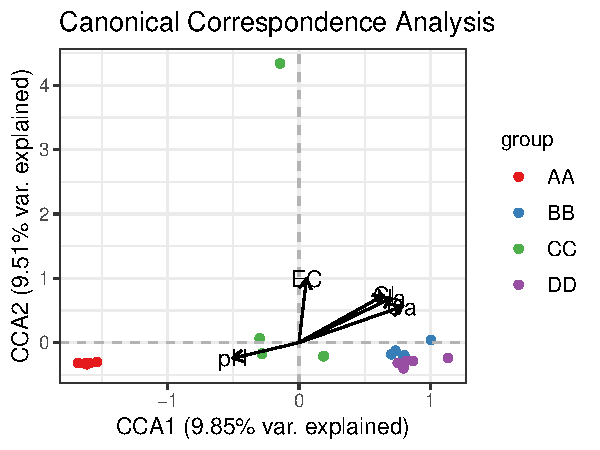
\includegraphics{workshop_files/figure-latex/unnamed-chunk-30-1.pdf}

\hypertarget{the-arch-effect-in-cca}{%
\paragraph{The arch effect in CCA}\label{the-arch-effect-in-cca}}

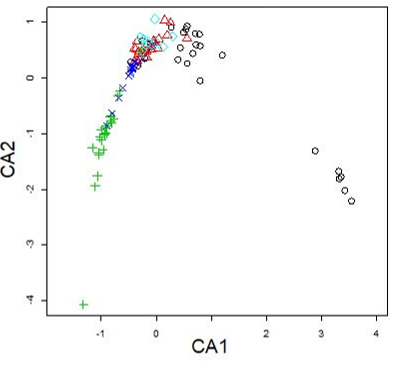
\includegraphics[width=0.7\textwidth,height=\textheight]{images/Fig11.png}

A common artifact in CCA is the arch effect, a curvature in the
ordination space that arises when species distributions follow strong
unimodal patterns. This occurs because Chi-square distances emphasize
differences in species presence and absence, leading to distortions in
the ordination space. As a result, sites along a continuous
environmental gradient may appear curved instead of following a linear
progression.

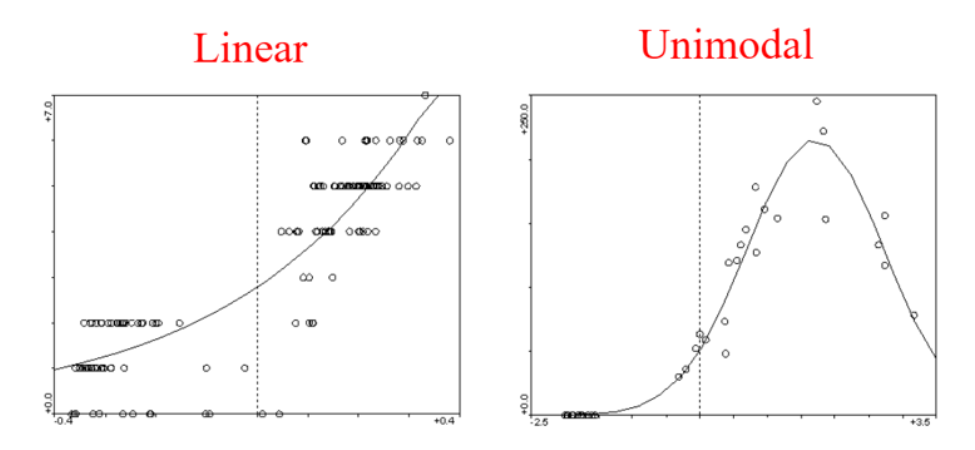
\includegraphics[width=0.8\textwidth,height=\textheight]{images/Fig12.png}

x-axis is environmental gradient and y-axis is abundance of species.

reference :

\begin{itemize}
\item
  \href{https://www.davidzeleny.net/anadat-r/doku.php/en:ca_dca}{David
  Zelený Lab at NTU}
\item
  \href{https://slideplayer.com/slide/776318/}{slideplayer}
\end{itemize}

\hypertarget{dca}{%
\subsection{DCA}\label{dca}}

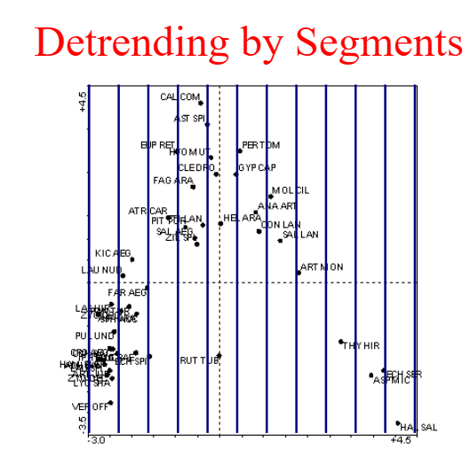
\includegraphics[width=0.6\textwidth,height=\textheight]{images/Fig13.png}

To correct the arch effect, Detrended Correspondence Analysis (DCA) was
introduced. DCA is a modification of Correspondence Analysis (CA) that
removes the arch effect through segment-wise detrending and local
standardization.

\hypertarget{segment-wise-detrending}{%
\paragraph{Segment-wise Detrending}\label{segment-wise-detrending}}

DCA first computes an initial ordination using Correspondence Analysis
(CA). However, instead of allowing the first axis to curve, DCA splits
the axis into equal segments and removes the local mean within each
segment. This eliminates the arch effect and ensures that the ordination
axis follows a straight gradient.

\hypertarget{local-standardization}{%
\paragraph{Local Standardization}\label{local-standardization}}

In addition to detrending, DCA adjusts species scores to equalize
species variance across the axis. This prevents overemphasis on dominant
species and ensures that species with different dispersions are treated
equally.

\hypertarget{dca-first-axis-and-gradient-length}{%
\paragraph{DCA First Axis and Gradient
Length}\label{dca-first-axis-and-gradient-length}}

The \texttt{first\ DCA\ axis\ (DCA1)} represents the primary gradient in
species composition. The length of the axis, measured in standard
deviation (SD) units, indicates the degree of species turnover:

\begin{itemize}
\tightlist
\item
  If first axis length \textless{} 2 SD:
\end{itemize}

species distributions follow a linear pattern, making
\texttt{Redundancy\ Analysis\ (RDA)} more appropriate.

\begin{itemize}
\tightlist
\item
  If first axis length \textgreater{} 4 SD:
\end{itemize}

species distributions follow a unimodal response, meaning \texttt{CCA}
is the better choice.

\begin{Shaded}
\begin{Highlighting}[]
\NormalTok{DCA }\OtherTok{\textless{}{-}} \FunctionTok{decorana}\NormalTok{(}\FunctionTok{t}\NormalTok{(wetland\_rarefied))}
\NormalTok{DCA}
\DocumentationTok{\#\# }
\DocumentationTok{\#\# Call:}
\DocumentationTok{\#\# decorana(veg = t(wetland\_rarefied)) }
\DocumentationTok{\#\# }
\DocumentationTok{\#\# Detrended correspondence analysis with 26 segments.}
\DocumentationTok{\#\# Rescaling of axes with 4 iterations.}
\DocumentationTok{\#\# Total inertia (scaled Chi{-}square): 9.2689 }
\DocumentationTok{\#\# }
\DocumentationTok{\#\#                         DCA1   DCA2   DCA3   DCA4}
\DocumentationTok{\#\# Eigenvalues           0.9682 0.7771 0.6458 0.4624}
\DocumentationTok{\#\# Additive Eigenvalues  0.9682 0.7762 0.6419 0.4392}
\DocumentationTok{\#\# Decorana values       0.9693 0.8123 0.6090 0.3957}
\DocumentationTok{\#\# Axis lengths         12.8999 6.9736 5.7240 3.5045}
\end{Highlighting}
\end{Shaded}

\begin{Shaded}
\begin{Highlighting}[]
\CommentTok{\#dca\_factor \textless{}{-} envfit(as.formula(paste("DCA\textasciitilde{} ", paste(colnames(ion), collapse = " + "))), data = ion)}
\NormalTok{dca\_factor }\OtherTok{\textless{}{-}} \FunctionTok{envfit}\NormalTok{(DCA}\SpecialCharTok{\textasciitilde{}}\NormalTok{ Na }\SpecialCharTok{+}\NormalTok{ Ca }\SpecialCharTok{+}\NormalTok{ Cl}\SpecialCharTok{+}\NormalTok{ EC }\SpecialCharTok{+}\NormalTok{ Salinity }\SpecialCharTok{+}\NormalTok{ pH, }\AttributeTok{data =}\NormalTok{ ion)}
\NormalTok{dca\_factor}
\DocumentationTok{\#\# }
\DocumentationTok{\#\# ***VECTORS}
\DocumentationTok{\#\# }
\DocumentationTok{\#\#              DCA1     DCA2     r2 Pr(\textgreater{}r)   }
\DocumentationTok{\#\# Na       {-}0.99542 {-}0.09556 0.4575  0.008 **}
\DocumentationTok{\#\# Ca       {-}0.93041  0.36653 0.5559  0.002 **}
\DocumentationTok{\#\# Cl       {-}0.99632 {-}0.08571 0.3943  0.016 * }
\DocumentationTok{\#\# EC       {-}0.60555  0.79581 0.0241  0.773   }
\DocumentationTok{\#\# Salinity {-}0.99586 {-}0.09094 0.4272  0.011 * }
\DocumentationTok{\#\# pH        0.84129 {-}0.54058 0.3720  0.017 * }
\DocumentationTok{\#\# {-}{-}{-}}
\DocumentationTok{\#\# Signif. codes:  0 \textquotesingle{}***\textquotesingle{} 0.001 \textquotesingle{}**\textquotesingle{} 0.01 \textquotesingle{}*\textquotesingle{} 0.05 \textquotesingle{}.\textquotesingle{} 0.1 \textquotesingle{} \textquotesingle{} 1}
\DocumentationTok{\#\# Permutation: free}
\DocumentationTok{\#\# Number of permutations: 999}
\end{Highlighting}
\end{Shaded}

\begin{Shaded}
\begin{Highlighting}[]
\NormalTok{dcv }\OtherTok{\textless{}{-}} \FunctionTok{data.frame}\NormalTok{(dca\_factor}\SpecialCharTok{$}\NormalTok{vectors}\SpecialCharTok{$}\NormalTok{arrows)}
\NormalTok{DCA\_sum }\OtherTok{\textless{}{-}} \FunctionTok{as.data.frame}\NormalTok{(}\FunctionTok{summary}\NormalTok{(DCA)}\SpecialCharTok{$}\NormalTok{site.scores)}
\DocumentationTok{\#\# }
\DocumentationTok{\#\# Call:}
\DocumentationTok{\#\# decorana(veg = t(wetland\_rarefied)) }
\DocumentationTok{\#\# }
\DocumentationTok{\#\# Detrended correspondence analysis with 26 segments.}
\DocumentationTok{\#\# Rescaling of axes with 4 iterations.}
\DocumentationTok{\#\# Total inertia (scaled Chi{-}square): 9.2689 }
\DocumentationTok{\#\# }
\DocumentationTok{\#\#                         DCA1   DCA2   DCA3   DCA4}
\DocumentationTok{\#\# Eigenvalues           0.9682 0.7771 0.6458 0.4624}
\DocumentationTok{\#\# Additive Eigenvalues  0.9682 0.7762 0.6419 0.4392}
\DocumentationTok{\#\# Decorana values       0.9693 0.8123 0.6090 0.3957}
\DocumentationTok{\#\# Axis lengths         12.8999 6.9736 5.7240 3.5045}
\NormalTok{DCAscores }\OtherTok{\textless{}{-}}\NormalTok{ DCA\_sum }\SpecialCharTok{\%\textgreater{}\%} \FunctionTok{rownames\_to\_column}\NormalTok{(}\StringTok{"site"}\NormalTok{)}
\NormalTok{DCAscores}\SpecialCharTok{$}\NormalTok{group }\OtherTok{\textless{}{-}} \FunctionTok{substr}\NormalTok{(}\FunctionTok{rownames}\NormalTok{(ion),}\DecValTok{1}\NormalTok{,}\DecValTok{2}\NormalTok{)}

\FunctionTok{ggplot}\NormalTok{() }\SpecialCharTok{+} \FunctionTok{geom\_point}\NormalTok{(}\AttributeTok{data =}\NormalTok{ DCAscores, }\FunctionTok{aes}\NormalTok{(}\AttributeTok{x =}\NormalTok{ DCA1, }\AttributeTok{y =}\NormalTok{ DCA2, }\AttributeTok{color =}\NormalTok{ group), }\AttributeTok{alpha=}\DecValTok{1}\NormalTok{) }\SpecialCharTok{+}
    \FunctionTok{geom\_vline}\NormalTok{(}\AttributeTok{xintercept =} \FunctionTok{c}\NormalTok{(}\DecValTok{0}\NormalTok{), }\AttributeTok{color =} \StringTok{"grey70"}\NormalTok{, }\AttributeTok{linetype =} \DecValTok{2}\NormalTok{) }\SpecialCharTok{+}
    \FunctionTok{geom\_hline}\NormalTok{(}\AttributeTok{yintercept =} \FunctionTok{c}\NormalTok{(}\DecValTok{0}\NormalTok{), }\AttributeTok{color =} \StringTok{"grey70"}\NormalTok{, }\AttributeTok{linetype =} \DecValTok{2}\NormalTok{) }\SpecialCharTok{+}
    \FunctionTok{geom\_segment}\NormalTok{(}\AttributeTok{data =}\NormalTok{ dcv, }\FunctionTok{aes}\NormalTok{(}\AttributeTok{x =} \DecValTok{0}\NormalTok{, }\AttributeTok{y =} \DecValTok{0}\NormalTok{, }\AttributeTok{xend =}\NormalTok{ DCA1, }\AttributeTok{yend =}\NormalTok{ DCA2), }\AttributeTok{arrow =} \FunctionTok{arrow}\NormalTok{(}\AttributeTok{length =} \FunctionTok{unit}\NormalTok{(}\FloatTok{0.2}\NormalTok{, }\StringTok{"cm"}\NormalTok{))) }\SpecialCharTok{+}
    \FunctionTok{geom\_text}\NormalTok{(}\AttributeTok{data =}\NormalTok{ dcv, }\FunctionTok{aes}\NormalTok{(}\AttributeTok{x =}\NormalTok{ DCA1, }\AttributeTok{y =}\NormalTok{ DCA2, }\AttributeTok{label =} \FunctionTok{rownames}\NormalTok{(dcv))) }\SpecialCharTok{+} \FunctionTok{theme\_bw}\NormalTok{() }\SpecialCharTok{+}
    \FunctionTok{scale\_color\_brewer}\NormalTok{(}\AttributeTok{palette =} \StringTok{\textquotesingle{}Set1\textquotesingle{}}\NormalTok{) }\SpecialCharTok{+} 
    \FunctionTok{labs}\NormalTok{(}\AttributeTok{x =} \FunctionTok{paste0}\NormalTok{(}\StringTok{"DCA1 ("}\NormalTok{,}\FunctionTok{round}\NormalTok{(DCA}\SpecialCharTok{$}\NormalTok{evals[}\DecValTok{1}\NormalTok{] }\SpecialCharTok{/}\NormalTok{ DCA}\SpecialCharTok{$}\NormalTok{totchi}\SpecialCharTok{*}\DecValTok{100}\NormalTok{,}\DecValTok{2}\NormalTok{), }\StringTok{"\% var. explained)"}\NormalTok{),}
         \AttributeTok{y =} \FunctionTok{paste0}\NormalTok{(}\StringTok{"DCA2 ("}\NormalTok{,}\FunctionTok{round}\NormalTok{(DCA}\SpecialCharTok{$}\NormalTok{evals[}\DecValTok{2}\NormalTok{] }\SpecialCharTok{/}\NormalTok{ DCA}\SpecialCharTok{$}\NormalTok{totchi}\SpecialCharTok{*}\DecValTok{100}\NormalTok{,}\DecValTok{2}\NormalTok{), }\StringTok{"\% var. explained)"}\NormalTok{),}
         \AttributeTok{title =} \StringTok{"Detrended Correspondence Analysis"}\NormalTok{)}\SpecialCharTok{+}
    \FunctionTok{theme}\NormalTok{(}\AttributeTok{legend.text.align =} \DecValTok{0}\NormalTok{, }\AttributeTok{legend.title.align =} \DecValTok{0}\NormalTok{,}
      \AttributeTok{legend.title=}\FunctionTok{element\_text}\NormalTok{(}\AttributeTok{size=}\DecValTok{18}\NormalTok{),}
      \AttributeTok{legend.text=}\FunctionTok{element\_text}\NormalTok{(}\AttributeTok{size=}\DecValTok{18}\NormalTok{),}
      \AttributeTok{axis.text =} \FunctionTok{element\_text}\NormalTok{(}\AttributeTok{size=}\DecValTok{18}\NormalTok{))}
\end{Highlighting}
\end{Shaded}

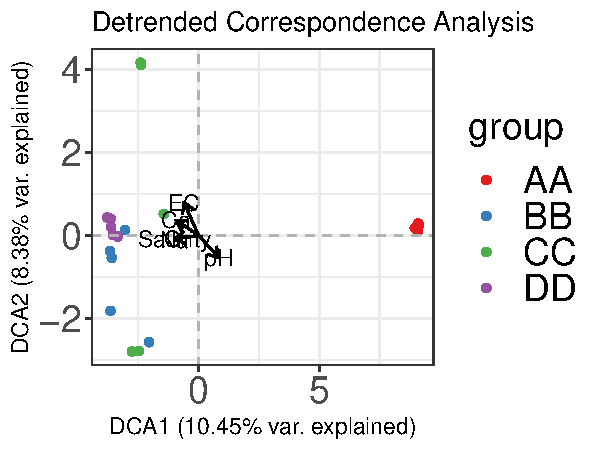
\includegraphics{workshop_files/figure-latex/unnamed-chunk-33-1.pdf}

\hypertarget{rda}{%
\subsection{RDA}\label{rda}}

Redundancy Analysis (RDA) is a linear constrained ordination method
similar to Principal Component Analysis (PCA), but with environmental
constraints. Instead of using Chi-square distances, RDA applies
Euclidean distances, making it suitable when species responses are
approximately linear with respect to environmental gradients.

Given a species data matrix and an environmental matrix , RDA performs a
multivariate regression of on , followed by PCA on the fitted values.
This results in ordination axes that explain the maximum variation in
species data constrained by the environmental variables.

\begin{Shaded}
\begin{Highlighting}[]
\CommentTok{\#RDA \textless{}{-} rda(as.formula(paste("t(wetland\_rarefied)\textasciitilde{} ", paste(colnames(ion), collapse = " + "))), ion)}
\NormalTok{RDA }\OtherTok{\textless{}{-}} \FunctionTok{rda}\NormalTok{(}\FunctionTok{t}\NormalTok{(wetland\_rarefied)}\SpecialCharTok{\textasciitilde{}}\NormalTok{ Na }\SpecialCharTok{+}\NormalTok{ Ca }\SpecialCharTok{+}\NormalTok{ Cl}\SpecialCharTok{+}\NormalTok{ EC }\SpecialCharTok{+}\NormalTok{ Salinity }\SpecialCharTok{+}\NormalTok{ pH, ion)}
\NormalTok{rda\_temp }\OtherTok{\textless{}{-}} \FunctionTok{anova.cca}\NormalTok{(RDA)}
\NormalTok{rda\_term }\OtherTok{\textless{}{-}} \FunctionTok{anova.cca}\NormalTok{(RDA, }\AttributeTok{by=}\StringTok{"terms"}\NormalTok{)}
\NormalTok{rda\_term}
\DocumentationTok{\#\# Permutation test for rda under reduced model}
\DocumentationTok{\#\# Terms added sequentially (first to last)}
\DocumentationTok{\#\# Permutation: free}
\DocumentationTok{\#\# Number of permutations: 999}
\DocumentationTok{\#\# }
\DocumentationTok{\#\# Model: rda(formula = t(wetland\_rarefied) \textasciitilde{} Na + Ca + Cl + EC + Salinity + pH, data = ion)}
\DocumentationTok{\#\#          Df Variance      F Pr(\textgreater{}F)    }
\DocumentationTok{\#\# Na        1   783986 2.3209  0.001 ***}
\DocumentationTok{\#\# Ca        1   541133 1.6020  0.051 .  }
\DocumentationTok{\#\# Cl        1   392550 1.1621  0.269    }
\DocumentationTok{\#\# EC        1   362663 1.0736  0.371    }
\DocumentationTok{\#\# pH        1   457295 1.3538  0.134    }
\DocumentationTok{\#\# Residual 14  4729101                  }
\DocumentationTok{\#\# {-}{-}{-}}
\DocumentationTok{\#\# Signif. codes:  0 \textquotesingle{}***\textquotesingle{} 0.001 \textquotesingle{}**\textquotesingle{} 0.01 \textquotesingle{}*\textquotesingle{} 0.05 \textquotesingle{}.\textquotesingle{} 0.1 \textquotesingle{} \textquotesingle{} 1}
\end{Highlighting}
\end{Shaded}

\begin{Shaded}
\begin{Highlighting}[]
\NormalTok{RDA\_sum }\OtherTok{\textless{}{-}} \FunctionTok{summary}\NormalTok{(RDA)}
\NormalTok{RDAscores }\OtherTok{\textless{}{-}} \FunctionTok{as.data.frame}\NormalTok{(RDA\_sum}\SpecialCharTok{$}\NormalTok{sites[,}\DecValTok{1}\SpecialCharTok{:}\DecValTok{2}\NormalTok{]) }\SpecialCharTok{\%\textgreater{}\%} \FunctionTok{rownames\_to\_column}\NormalTok{(}\StringTok{"site"}\NormalTok{)}
\NormalTok{RDAscores}\SpecialCharTok{$}\NormalTok{group }\OtherTok{\textless{}{-}} \FunctionTok{substr}\NormalTok{(}\FunctionTok{rownames}\NormalTok{(ion),}\DecValTok{1}\NormalTok{,}\DecValTok{2}\NormalTok{)}
\NormalTok{cc }\OtherTok{\textless{}{-}} \FunctionTok{as.data.frame}\NormalTok{(RDA\_sum}\SpecialCharTok{$}\NormalTok{biplot[,}\DecValTok{1}\SpecialCharTok{:}\DecValTok{2}\NormalTok{])}
\FunctionTok{ggplot}\NormalTok{() }\SpecialCharTok{+} \FunctionTok{geom\_point}\NormalTok{(}\AttributeTok{data =}\NormalTok{ RDAscores, }\FunctionTok{aes}\NormalTok{(}\AttributeTok{x =}\NormalTok{ RDA1, }\AttributeTok{y =}\NormalTok{ RDA2, }\AttributeTok{color=}\NormalTok{group), }\AttributeTok{alpha=}\DecValTok{1}\NormalTok{) }\SpecialCharTok{+}
    \FunctionTok{geom\_vline}\NormalTok{(}\AttributeTok{xintercept =} \FunctionTok{c}\NormalTok{(}\DecValTok{0}\NormalTok{), }\AttributeTok{color =} \StringTok{"grey70"}\NormalTok{, }\AttributeTok{linetype =} \DecValTok{2}\NormalTok{) }\SpecialCharTok{+}
    \FunctionTok{geom\_hline}\NormalTok{(}\AttributeTok{yintercept =} \FunctionTok{c}\NormalTok{(}\DecValTok{0}\NormalTok{), }\AttributeTok{color =} \StringTok{"grey70"}\NormalTok{, }\AttributeTok{linetype =} \DecValTok{2}\NormalTok{) }\SpecialCharTok{+}
    \FunctionTok{geom\_segment}\NormalTok{(}\AttributeTok{data =}\NormalTok{ cc, }\FunctionTok{aes}\NormalTok{(}\AttributeTok{x =} \DecValTok{0}\NormalTok{, }\AttributeTok{y =} \DecValTok{0}\NormalTok{, }\AttributeTok{xend =}\NormalTok{ RDA1, }\AttributeTok{yend =}\NormalTok{ RDA2), }\AttributeTok{arrow =} \FunctionTok{arrow}\NormalTok{(}\AttributeTok{length =} \FunctionTok{unit}\NormalTok{(}\FloatTok{0.2}\NormalTok{, }\StringTok{"cm"}\NormalTok{))) }\SpecialCharTok{+}
    \FunctionTok{geom\_text}\NormalTok{(}\AttributeTok{data =}\NormalTok{ cc, }\FunctionTok{aes}\NormalTok{(}\AttributeTok{x =}\NormalTok{ RDA1, }\AttributeTok{y =}\NormalTok{ RDA2, }\AttributeTok{label =} \FunctionTok{rownames}\NormalTok{(cc))) }\SpecialCharTok{+} \FunctionTok{theme\_bw}\NormalTok{() }\SpecialCharTok{+}
    \FunctionTok{scale\_color\_brewer}\NormalTok{(}\AttributeTok{palette =} \StringTok{\textquotesingle{}Set1\textquotesingle{}}\NormalTok{)  }\SpecialCharTok{+}
    \FunctionTok{labs}\NormalTok{(}\AttributeTok{x =} \FunctionTok{paste0}\NormalTok{(}\StringTok{"RDA1 ("}\NormalTok{,}\FunctionTok{round}\NormalTok{(RDA}\SpecialCharTok{$}\NormalTok{CCA}\SpecialCharTok{$}\NormalTok{eig[}\DecValTok{1}\NormalTok{] }\SpecialCharTok{/}\NormalTok{ RDA}\SpecialCharTok{$}\NormalTok{tot.chi}\SpecialCharTok{*}\DecValTok{100}\NormalTok{,}\DecValTok{2}\NormalTok{), }\StringTok{"\% var. explained)"}\NormalTok{),}
         \AttributeTok{y =} \FunctionTok{paste0}\NormalTok{(}\StringTok{"RDA2 ("}\NormalTok{,}\FunctionTok{round}\NormalTok{(RDA}\SpecialCharTok{$}\NormalTok{CCA}\SpecialCharTok{$}\NormalTok{eig[}\DecValTok{2}\NormalTok{] }\SpecialCharTok{/}\NormalTok{ RDA}\SpecialCharTok{$}\NormalTok{tot.chi}\SpecialCharTok{*}\DecValTok{100}\NormalTok{,}\DecValTok{2}\NormalTok{), }\StringTok{"\% var. explained)"}\NormalTok{),}
         \AttributeTok{title =} \StringTok{"Redundancy Analysis"}\NormalTok{) }\SpecialCharTok{+}
    \FunctionTok{theme}\NormalTok{(}\AttributeTok{legend.text.align =} \DecValTok{0}\NormalTok{, }\AttributeTok{legend.title.align =} \DecValTok{0}\NormalTok{,}
          \AttributeTok{legend.title=}\FunctionTok{element\_text}\NormalTok{(}\AttributeTok{size=}\DecValTok{10}\NormalTok{),}\AttributeTok{legend.text=}\FunctionTok{element\_text}\NormalTok{(}\AttributeTok{size=}\DecValTok{10}\NormalTok{))}
\end{Highlighting}
\end{Shaded}

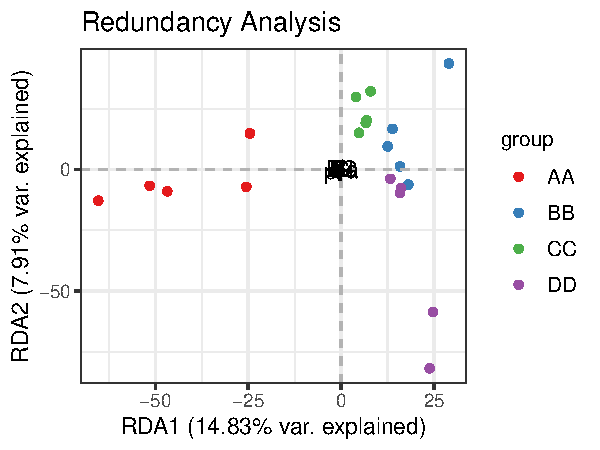
\includegraphics{workshop_files/figure-latex/unnamed-chunk-35-1.pdf}

\hypertarget{differential-taxa}{%
\section{Differential Taxa}\label{differential-taxa}}

\hypertarget{aldex2}{%
\subsection{ALDEx2}\label{aldex2}}

\href{https://microbiomejournal.biomedcentral.com/articles/10.1186/2049-2618-2-15}{ALDEx2}
which generated Monte Carlo samples of Dirichlet distributions for each
sample, using a uniform prior, performed CLR transformation of each
realization, and then performed Wilcoxon tests on the transformed
realizations.

\begin{Shaded}
\begin{Highlighting}[]
\FunctionTok{library}\NormalTok{(ALDEx2)}
\DocumentationTok{\#\# Loading required package: zCompositions}
\DocumentationTok{\#\# Loading required package: MASS}
\DocumentationTok{\#\# }
\DocumentationTok{\#\# Attaching package: \textquotesingle{}MASS\textquotesingle{}}
\DocumentationTok{\#\# The following object is masked from \textquotesingle{}package:rstatix\textquotesingle{}:}
\DocumentationTok{\#\# }
\DocumentationTok{\#\#     select}
\DocumentationTok{\#\# The following object is masked from \textquotesingle{}package:patchwork\textquotesingle{}:}
\DocumentationTok{\#\# }
\DocumentationTok{\#\#     area}
\DocumentationTok{\#\# The following object is masked from \textquotesingle{}package:dplyr\textquotesingle{}:}
\DocumentationTok{\#\# }
\DocumentationTok{\#\#     select}
\DocumentationTok{\#\# Loading required package: NADA}
\DocumentationTok{\#\# Loading required package: survival}
\DocumentationTok{\#\# }
\DocumentationTok{\#\# Attaching package: \textquotesingle{}NADA\textquotesingle{}}
\DocumentationTok{\#\# The following object is masked from \textquotesingle{}package:IRanges\textquotesingle{}:}
\DocumentationTok{\#\# }
\DocumentationTok{\#\#     cor}
\DocumentationTok{\#\# The following object is masked from \textquotesingle{}package:S4Vectors\textquotesingle{}:}
\DocumentationTok{\#\# }
\DocumentationTok{\#\#     cor}
\DocumentationTok{\#\# The following object is masked from \textquotesingle{}package:stats\textquotesingle{}:}
\DocumentationTok{\#\# }
\DocumentationTok{\#\#     cor}
\DocumentationTok{\#\# Loading required package: truncnorm}
\NormalTok{ALDEx2\_result }\OtherTok{\textless{}{-}} \FunctionTok{aldex}\NormalTok{(}\AttributeTok{reads=}\NormalTok{data, }\AttributeTok{conditions =}\NormalTok{ meta}\SpecialCharTok{$}\NormalTok{Class,}
                       \AttributeTok{mc.samples =} \DecValTok{128}\NormalTok{, }\AttributeTok{test=}\StringTok{"t"}\NormalTok{, }\AttributeTok{effect=}\ConstantTok{TRUE}\NormalTok{,}
                       \AttributeTok{include.sample.summary =} \ConstantTok{FALSE}\NormalTok{, }\AttributeTok{verbose=}\NormalTok{T, }\AttributeTok{denom=}\StringTok{"all"}\NormalTok{)}
\DocumentationTok{\#\# aldex.clr: generating Monte{-}Carlo instances and clr values}
\DocumentationTok{\#\# operating in serial mode}
\DocumentationTok{\#\# removed rows with sums equal to zero}
\DocumentationTok{\#\# computing center with all features}
\DocumentationTok{\#\# data format is OK}
\DocumentationTok{\#\# dirichlet samples complete}
\DocumentationTok{\#\# transformation complete}
\DocumentationTok{\#\# aldex.ttest: doing t{-}test}
\DocumentationTok{\#\# running tests for each MC instance:}
\DocumentationTok{\#\# |{-}{-}{-}{-}{-}{-}{-}{-}{-}{-}{-}{-}(25\%){-}{-}{-}{-}{-}{-}{-}{-}{-}{-}(50\%){-}{-}{-}{-}{-}{-}{-}{-}{-}{-}(75\%){-}{-}{-}{-}{-}{-}{-}{-}{-}{-}|}
\DocumentationTok{\#\# aldex.effect: calculating effect sizes}
\DocumentationTok{\#\# operating in serial mode}
\DocumentationTok{\#\# sanity check complete}
\DocumentationTok{\#\# rab.all  complete}
\DocumentationTok{\#\# rab.win  complete}
\DocumentationTok{\#\# rab of samples complete}
\DocumentationTok{\#\# within sample difference calculated}
\DocumentationTok{\#\# between group difference calculated}
\DocumentationTok{\#\# group summaries calculated}
\DocumentationTok{\#\# effect size calculated}
\DocumentationTok{\#\# summarizing output}

\NormalTok{selected\_result }\OtherTok{\textless{}{-}}\NormalTok{ ALDEx2\_result[ALDEx2\_result}\SpecialCharTok{$}\NormalTok{wi.ep }\SpecialCharTok{\textless{}} \FloatTok{0.05}\NormalTok{,]}
\NormalTok{selected\_result }\OtherTok{\textless{}{-}} \FunctionTok{cbind}\NormalTok{(}\FunctionTok{rownames}\NormalTok{(selected\_result),selected\_result)}
\FunctionTok{head}\NormalTok{(selected\_result)}
\DocumentationTok{\#\#         rownames(selected\_result)   rab.all rab.win.Cancer rab.win.Normal}
\DocumentationTok{\#\# ASV0001                   ASV0001 14.373547      14.630241     13.8742929}
\DocumentationTok{\#\# ASV0007                   ASV0007  9.648390      12.282246      7.7414882}
\DocumentationTok{\#\# ASV0119                   ASV0119  8.466592       3.945452     10.0351473}
\DocumentationTok{\#\# ASV0130                   ASV0130  3.991660       1.643844      9.4433972}
\DocumentationTok{\#\# ASV0146                   ASV0146  8.222159       9.565661      7.4461137}
\DocumentationTok{\#\# ASV0178                   ASV0178  1.850530       5.716942      0.4256441}
\DocumentationTok{\#\#          diff.btw diff.win     effect   overlap       we.ep    we.eBH}
\DocumentationTok{\#\# ASV0001 {-}1.377995 2.364327 {-}0.5127501 0.3161593 0.009924686 0.9111672}
\DocumentationTok{\#\# ASV0007 {-}4.198266 5.508847 {-}0.6886866 0.2265625 0.001738385 0.8659766}
\DocumentationTok{\#\# ASV0119  4.845204 7.793662  0.6220667 0.2638564 0.008007031 0.8930373}
\DocumentationTok{\#\# ASV0130  4.215072 9.212734  0.4781253 0.3099141 0.056589218 0.9238886}
\DocumentationTok{\#\# ASV0146 {-}1.937207 5.932652 {-}0.3029744 0.3093750 0.149241061 0.9396661}
\DocumentationTok{\#\# ASV0178 {-}5.289013 6.269317 {-}0.7701952 0.2107729 0.003434822 0.7223806}
\DocumentationTok{\#\#               wi.ep    wi.eBH}
\DocumentationTok{\#\# ASV0001 0.041240625 0.9270136}
\DocumentationTok{\#\# ASV0007 0.003136204 0.8139919}
\DocumentationTok{\#\# ASV0119 0.009039480 0.8642710}
\DocumentationTok{\#\# ASV0130 0.049115638 0.9198037}
\DocumentationTok{\#\# ASV0146 0.046041349 0.9261615}
\DocumentationTok{\#\# ASV0178 0.003249730 0.6543478}
\CommentTok{\#write.table(selected\_result, "\textasciitilde{}/Course/NDMC\_2025/tmp/ALDEx2.txt", quote=FALSE, sep="\textbackslash{}t", col.names = F, row.names = F)}
\end{Highlighting}
\end{Shaded}

\hypertarget{ancom}{%
\subsection{ANCOM}\label{ancom}}

\href{https://www.frontiersin.org/articles/10.3389/fmicb.2017.02114/full}{ANCOM}
first examined the abundance table to identify \texttt{outlier\ zeros}
and \texttt{structural\ zeros}, Outlier zeros, identified by finding
outliers in the distribution of taxon counts within each sample
grouping, were ignored during differential abundance analysis, and
replaced with NA. Structural zeros, taxa that were absent in one
grouping but present in the other, were ignored during data analysis and
automatically called as differentially abundant. Using the main function
ANCOM, all additive log-ratios for each taxon were then tested for
significance using Wilcoxon rank-sum tests, and p-values were
FDR-corrected using the BH method. ANCOM-II then applied a detection
threshold as described in the
\href{https://www.ncbi.nlm.nih.gov/pmc/articles/PMC4450248/}{original
paper}, whereby a taxon was called as DA if the number of corrected
p-values reaching nominal significance for that taxon was greater than
60\% of the maximum possible number of significant comparisons.

\begin{Shaded}
\begin{Highlighting}[]
\FunctionTok{library}\NormalTok{(compositions)}
\DocumentationTok{\#\# Welcome to compositions, a package for compositional data analysis.}
\DocumentationTok{\#\# Find an intro with "? compositions"}
\DocumentationTok{\#\# }
\DocumentationTok{\#\# Attaching package: \textquotesingle{}compositions\textquotesingle{}}
\DocumentationTok{\#\# The following object is masked from \textquotesingle{}package:NADA\textquotesingle{}:}
\DocumentationTok{\#\# }
\DocumentationTok{\#\#     cor}
\DocumentationTok{\#\# The following object is masked from \textquotesingle{}package:ape\textquotesingle{}:}
\DocumentationTok{\#\# }
\DocumentationTok{\#\#     balance}
\DocumentationTok{\#\# The following objects are masked from \textquotesingle{}package:IRanges\textquotesingle{}:}
\DocumentationTok{\#\# }
\DocumentationTok{\#\#     cor, cov, var}
\DocumentationTok{\#\# The following objects are masked from \textquotesingle{}package:S4Vectors\textquotesingle{}:}
\DocumentationTok{\#\# }
\DocumentationTok{\#\#     cor, cov, var}
\DocumentationTok{\#\# The following objects are masked from \textquotesingle{}package:BiocGenerics\textquotesingle{}:}
\DocumentationTok{\#\# }
\DocumentationTok{\#\#     normalize, var}
\DocumentationTok{\#\# The following objects are masked from \textquotesingle{}package:stats\textquotesingle{}:}
\DocumentationTok{\#\# }
\DocumentationTok{\#\#     anova, cor, cov, dist, var}
\DocumentationTok{\#\# The following object is masked from \textquotesingle{}package:graphics\textquotesingle{}:}
\DocumentationTok{\#\# }
\DocumentationTok{\#\#     segments}
\DocumentationTok{\#\# The following objects are masked from \textquotesingle{}package:base\textquotesingle{}:}
\DocumentationTok{\#\# }
\DocumentationTok{\#\#     \%*\%, norm, scale, scale.default}
\FunctionTok{library}\NormalTok{(exactRankTests)}
\DocumentationTok{\#\#  Package \textquotesingle{}exactRankTests\textquotesingle{} is no longer under development.}
\DocumentationTok{\#\#  Please consider using package \textquotesingle{}coin\textquotesingle{} instead.}
\FunctionTok{library}\NormalTok{(nlme)}
\FunctionTok{source}\NormalTok{(}\StringTok{\textquotesingle{}\textasciitilde{}/Course/NDMC\_2025/source/ancom\_v2.1.R\textquotesingle{}}\NormalTok{)}

\NormalTok{meta}\SpecialCharTok{$}\NormalTok{Sample }\OtherTok{\textless{}{-}} \FunctionTok{rownames}\NormalTok{(meta)}
\NormalTok{prepro }\OtherTok{\textless{}{-}} \FunctionTok{feature\_table\_pre\_process}\NormalTok{(}\AttributeTok{feature\_table =}\NormalTok{ data, }\AttributeTok{meta\_data =}\NormalTok{ meta,}
                                    \AttributeTok{sample\_var =} \StringTok{\textquotesingle{}Sample\textquotesingle{}}\NormalTok{, }\AttributeTok{group\_var =} \StringTok{\textquotesingle{}Class\textquotesingle{}}\NormalTok{,}
                                    \AttributeTok{out\_cut =} \FloatTok{0.05}\NormalTok{, }\AttributeTok{zero\_cut =} \FloatTok{0.90}\NormalTok{,}
                                    \AttributeTok{lib\_cut =} \DecValTok{1000}\NormalTok{, }\AttributeTok{neg\_lb=}\ConstantTok{FALSE}\NormalTok{)}
\NormalTok{feature\_table }\OtherTok{\textless{}{-}}\NormalTok{ prepro}\SpecialCharTok{$}\NormalTok{feature\_table}
\NormalTok{metadata }\OtherTok{\textless{}{-}}\NormalTok{ prepro}\SpecialCharTok{$}\NormalTok{meta\_data}
\NormalTok{struc\_zero }\OtherTok{\textless{}{-}}\NormalTok{ prepro}\SpecialCharTok{$}\NormalTok{structure\_zeros}
\NormalTok{main\_var }\OtherTok{\textless{}{-}} \StringTok{\textquotesingle{}Class\textquotesingle{}}
\NormalTok{p\_adj\_method }\OtherTok{=} \StringTok{"BH"}
\NormalTok{alpha}\OtherTok{=}\FloatTok{0.05}
\NormalTok{adj\_formula}\OtherTok{=}\ConstantTok{NULL}
\NormalTok{rand\_formula}\OtherTok{=}\ConstantTok{NULL}
\NormalTok{ANCOM\_result }\OtherTok{\textless{}{-}} \FunctionTok{ANCOM}\NormalTok{(}\AttributeTok{feature\_table =}\NormalTok{ feature\_table, }\AttributeTok{meta\_data =}\NormalTok{ metadata,}
             \AttributeTok{struc\_zero =}\NormalTok{ struc\_zero, }\AttributeTok{main\_var =}\NormalTok{ main\_var, }\AttributeTok{p\_adj\_method =}\NormalTok{ p\_adj\_method,}
             \AttributeTok{alpha=}\NormalTok{alpha, }\AttributeTok{adj\_formula =}\NormalTok{ adj\_formula, }\AttributeTok{rand\_formula =}\NormalTok{ rand\_formula)}
\NormalTok{ANCOM\_result }\OtherTok{\textless{}{-}}\NormalTok{ ANCOM\_result}\SpecialCharTok{$}\NormalTok{out}
\NormalTok{ANCOM\_result }\OtherTok{\textless{}{-}}\NormalTok{ ANCOM\_result[ANCOM\_result}\SpecialCharTok{$}\NormalTok{W }\SpecialCharTok{!=} \DecValTok{0}\NormalTok{, ]}
\FunctionTok{head}\NormalTok{(ANCOM\_result)}
\DocumentationTok{\#\#     taxa\_id   W detected\_0.9 detected\_0.8 detected\_0.7 detected\_0.6}
\DocumentationTok{\#\# 6   ASV0007 457        FALSE        FALSE         TRUE         TRUE}
\DocumentationTok{\#\# 28  ASV0030   1        FALSE        FALSE        FALSE        FALSE}
\DocumentationTok{\#\# 40  ASV0042   1        FALSE        FALSE        FALSE        FALSE}
\DocumentationTok{\#\# 43  ASV0045   3        FALSE        FALSE        FALSE        FALSE}
\DocumentationTok{\#\# 103 ASV0119 467        FALSE        FALSE         TRUE         TRUE}
\DocumentationTok{\#\# 113 ASV0130   2        FALSE        FALSE        FALSE        FALSE}
\CommentTok{\#write.table(out, "\textasciitilde{}/Course/NDMC\_2025/tmp/ANCOM.txt", quote=FALSE, sep="\textbackslash{}t", col.names = F, row.names = F)}

\NormalTok{ANCOM\_selected }\OtherTok{\textless{}{-}}\NormalTok{ ANCOM\_result[ANCOM\_result}\SpecialCharTok{$}\NormalTok{detected\_0}\FloatTok{.6}\NormalTok{, ]}
\FunctionTok{head}\NormalTok{(ANCOM\_selected)}
\DocumentationTok{\#\#     taxa\_id   W detected\_0.9 detected\_0.8 detected\_0.7 detected\_0.6}
\DocumentationTok{\#\# 6   ASV0007 457        FALSE        FALSE         TRUE         TRUE}
\DocumentationTok{\#\# 103 ASV0119 467        FALSE        FALSE         TRUE         TRUE}
\DocumentationTok{\#\# 155 ASV0178 495        FALSE        FALSE         TRUE         TRUE}
\DocumentationTok{\#\# 182 ASV0222 395        FALSE        FALSE        FALSE         TRUE}
\DocumentationTok{\#\# 255 ASV0323 Inf         TRUE         TRUE         TRUE         TRUE}
\DocumentationTok{\#\# 468 ASV0842 Inf         TRUE         TRUE         TRUE         TRUE}
\CommentTok{\#write.table(out, "\textasciitilde{}/Course/NDMC\_2025/tmp/ANCOM\_thr.txt", quote=FALSE, sep="\textbackslash{}t", col.names = F, row.names = F)}
\end{Highlighting}
\end{Shaded}

\hypertarget{edger}{%
\subsection{edgeR}\label{edger}}

We added a pseudocount of 1 to the data and used the function
\texttt{calcNormFactors} from the
\href{https://genomebiology.biomedcentral.com/articles/10.1186/gb-2010-11-3-r25}{edgeR}
to compute relative log expression normalization factors. Negative
binomial dispersion parameters were then estimated using the functions
\texttt{estimateCommonDisp} followed by \texttt{estimateTagwiseDisp} to
shrink feature-wise dispersion estimates through an empirical Bayes
approach. We then used the \texttt{exactTest} for negative binomial data
to identify features that differ between the specified groups. The
resulting p-values were then corrected for multiple testing with the BH
method with the function \texttt{topTags}.

\begin{Shaded}
\begin{Highlighting}[]
\FunctionTok{library}\NormalTok{(edgeR)}
\DocumentationTok{\#\# Loading required package: limma}
\DocumentationTok{\#\# }
\DocumentationTok{\#\# Attaching package: \textquotesingle{}limma\textquotesingle{}}
\DocumentationTok{\#\# The following object is masked from \textquotesingle{}package:BiocGenerics\textquotesingle{}:}
\DocumentationTok{\#\# }
\DocumentationTok{\#\#     plotMA}

\NormalTok{ASV }\OtherTok{\textless{}{-}}\NormalTok{ phyloseq}\SpecialCharTok{::}\FunctionTok{otu\_table}\NormalTok{(data, }\AttributeTok{taxa\_are\_rows =}\NormalTok{ T)}
\NormalTok{sampledata }\OtherTok{\textless{}{-}}\NormalTok{ phyloseq}\SpecialCharTok{::}\FunctionTok{sample\_data}\NormalTok{(meta, }\AttributeTok{errorIfNULL =}\NormalTok{ T)}
\NormalTok{phylo }\OtherTok{\textless{}{-}}\NormalTok{ phyloseq}\SpecialCharTok{::}\FunctionTok{merge\_phyloseq}\NormalTok{(ASV, sampledata)}
\NormalTok{test }\OtherTok{\textless{}{-}} \FunctionTok{phyloseq\_to\_edgeR}\NormalTok{(}\AttributeTok{physeq =}\NormalTok{ phylo, }\AttributeTok{group =} \StringTok{"Class"}\NormalTok{) }\CommentTok{\# phyloseq\_to\_edgeR function is sourced from utils.R}
\NormalTok{et }\OtherTok{=} \FunctionTok{exactTest}\NormalTok{(test)}
\NormalTok{out }\OtherTok{=} \FunctionTok{topTags}\NormalTok{(et, }\AttributeTok{n=}\FunctionTok{nrow}\NormalTok{(test}\SpecialCharTok{$}\NormalTok{table), }\AttributeTok{adjust.method=}\StringTok{"BH"}\NormalTok{, }\AttributeTok{sort.by=}\StringTok{"PValue"}\NormalTok{)}
\NormalTok{edgeR\_result }\OtherTok{\textless{}{-}}\NormalTok{ out}\SpecialCharTok{@}\NormalTok{.Data[[}\DecValTok{1}\NormalTok{]]}
\NormalTok{edgeR\_selected }\OtherTok{\textless{}{-}}\NormalTok{ edgeR\_result[edgeR\_result}\SpecialCharTok{$}\NormalTok{FDR }\SpecialCharTok{\textless{}} \FloatTok{0.05}\NormalTok{,]}
\NormalTok{edgeR\_selected }\OtherTok{\textless{}{-}} \FunctionTok{cbind}\NormalTok{(}\FunctionTok{rownames}\NormalTok{(edgeR\_selected), edgeR\_selected)}
\FunctionTok{head}\NormalTok{(edgeR\_selected)}
\DocumentationTok{\#\#         rownames(edgeR\_selected)      logFC    logCPM       PValue          FDR}
\DocumentationTok{\#\# ASV0075                  ASV0075 {-}10.005478 11.509109 4.983343e{-}12 1.089973e{-}08}
\DocumentationTok{\#\# ASV0029                  ASV0029 {-}11.378337 12.878259 6.000401e{-}12 1.089973e{-}08}
\DocumentationTok{\#\# ASV0178                  ASV0178  {-}7.512891  9.946950 1.006243e{-}11 1.218560e{-}08}
\DocumentationTok{\#\# ASV0073                  ASV0073 {-}10.009413 11.513042 3.960265e{-}11 2.895228e{-}08}
\DocumentationTok{\#\# ASV0083                  ASV0083  {-}9.866453 11.370704 4.697678e{-}11 2.895228e{-}08}
\DocumentationTok{\#\# ASV0198                  ASV0198  {-}8.189402  9.708196 5.451478e{-}11 2.895228e{-}08}

\CommentTok{\# write.table(subout, "\textasciitilde{}/Course/NDMC\_2025/tmp/edgeR.txt", quote=FALSE, sep="\textbackslash{}t", col.names = F, row.names = F)}
\end{Highlighting}
\end{Shaded}

\hypertarget{lefse}{%
\subsection{LEfSe}\label{lefse}}

\href{https://pubmed.ncbi.nlm.nih.gov/21702898/}{LEfSe} performed a
Kruskal-Wallis (which in our two-group case reduces to the Wilcoxon
rank-sum) hypothesis test to identify potential differentially abundant
features, followed by linear discriminant analysis (LDA) of class labels
on abundances to estimate the effect sizes for significant features.
From these, only those features with scaled LDA analysis scores above
the threshold score of 2.0 (default) were called as differentially
abundant.

\begin{Shaded}
\begin{Highlighting}[]
\CommentTok{\# file preparation}
\NormalTok{ret\_tab }\OtherTok{\textless{}{-}} \FunctionTok{LEfSe\_preparation}\NormalTok{(data, taxa, meta, }\StringTok{"Class"}\NormalTok{, }\AttributeTok{pvl\_filter =} \FloatTok{0.05}\NormalTok{)}
\FunctionTok{head}\NormalTok{(ret\_tab[,}\DecValTok{1}\SpecialCharTok{:}\DecValTok{5}\NormalTok{])}
\DocumentationTok{\#\#                             [,1]               [,2]                }
\DocumentationTok{\#\# Class                       "Normal"           "Normal"            }
\DocumentationTok{\#\# sampleID                    "ERR475473"        "ERR475476"         }
\DocumentationTok{\#\# k\_Bacteria                  "90.4988091187479" "93.7881847531094"  }
\DocumentationTok{\#\# k\_Archaea                   "0"                "0.0237951303587277"}
\DocumentationTok{\#\# k\_Bacteria|p\_Proteobacteria "13.0343654304185" "6.13142629297594"  }
\DocumentationTok{\#\# k\_Bacteria|p\_Firmicutes     "58.7764545763865" "40.1578195943252"  }
\DocumentationTok{\#\#                             [,3]               [,4]              }
\DocumentationTok{\#\# Class                       "Normal"           "Normal"          }
\DocumentationTok{\#\# sampleID                    "ERR475478"        "ERR475480"       }
\DocumentationTok{\#\# k\_Bacteria                  "89.5623741239996" "98.1584169974317"}
\DocumentationTok{\#\# k\_Archaea                   "3.39050176528261" "0"               }
\DocumentationTok{\#\# k\_Bacteria|p\_Proteobacteria "6.6023018705717"  "16.199217837964" }
\DocumentationTok{\#\# k\_Bacteria|p\_Firmicutes     "71.9902052171225" "69.8721690403923"}
\DocumentationTok{\#\#                             [,5]              }
\DocumentationTok{\#\# Class                       "Normal"          }
\DocumentationTok{\#\# sampleID                    "ERR475483"       }
\DocumentationTok{\#\# k\_Bacteria                  "98.2261609156035"}
\DocumentationTok{\#\# k\_Archaea                   "0"               }
\DocumentationTok{\#\# k\_Bacteria|p\_Proteobacteria "7.60909895253589"}
\DocumentationTok{\#\# k\_Bacteria|p\_Firmicutes     "88.7233496018495"}

\FunctionTok{dir.create}\NormalTok{(}\StringTok{"\textasciitilde{}/Course/NDMC\_2025/tmp/LEfSe\_tmp"}\NormalTok{)}
\FunctionTok{write.table}\NormalTok{(ret\_tab, }\StringTok{"\textasciitilde{}/Course/NDMC\_2025/tmp/LEfSe\_tmp/tmp\_in.txt"}\NormalTok{, }\AttributeTok{quote=}\ConstantTok{FALSE}\NormalTok{, }\AttributeTok{sep=}\StringTok{"}\SpecialCharTok{\textbackslash{}t}\StringTok{"}\NormalTok{, }\AttributeTok{col.names =}\NormalTok{ F)}
\end{Highlighting}
\end{Shaded}

\begin{Shaded}
\begin{Highlighting}[]
\CommentTok{\# LEfSe execution by docker}
\ExtensionTok{$}\NormalTok{ docker run }\AttributeTok{{-}u} \VariableTok{$UID}\NormalTok{:}\VariableTok{$(}\FunctionTok{id} \AttributeTok{{-}g}\VariableTok{)} \AttributeTok{{-}it} \AttributeTok{{-}{-}rm} \AttributeTok{{-}v}\NormalTok{ /home/yincheng23/Course/NDMC\_2025/tmp/LEfSe\_tmp:/tmp yincheng23/lefse:0.0.4}
\ExtensionTok{$}\NormalTok{ format\_input.py /tmp/tmp\_in.txt /tmp/data\_in }\AttributeTok{{-}s} \AttributeTok{{-}1} \AttributeTok{{-}u}\NormalTok{ 2 }\AttributeTok{{-}o}\NormalTok{ 1000000}
\ExtensionTok{$}\NormalTok{ run\_lefse.py /tmp/data\_in /tmp/LEfSe\_res.txt}
\ExtensionTok{$}\NormalTok{ plot\_res.py /tmp/LEfSe\_res.txt /tmp/LEfSe\_res.png }\AttributeTok{{-}{-}dpi}\NormalTok{ 100}
\ExtensionTok{$}\NormalTok{ plot\_cladogram.py /tmp/LEfSe\_res.txt /tmp/cladogram.png }\AttributeTok{{-}{-}format}\NormalTok{ png }\AttributeTok{{-}{-}dpi}\NormalTok{ 100}
\ExtensionTok{$}\NormalTok{ cat /tmp/LEfSe\_res.txt }\KeywordTok{|} \FunctionTok{awk} \StringTok{\textquotesingle{}\{if($3\textgreater{}2)\{print $0\}\}\textquotesingle{}} \OperatorTok{\textgreater{}}\NormalTok{ /tmp/LEfSe\_res\_selected.txt  }\CommentTok{\# filtering by |LDA| \textgreater{} 2 and p \textless{} 0.05}
\end{Highlighting}
\end{Shaded}

\begin{Shaded}
\begin{Highlighting}[]
\NormalTok{result }\OtherTok{\textless{}{-}} \FunctionTok{read.csv}\NormalTok{(}\StringTok{"\textasciitilde{}/Course/NDMC\_2025/tmp/LEfSe\_tmp/LEfSe\_res.txt"}\NormalTok{, }\AttributeTok{sep =} \StringTok{\textquotesingle{}}\SpecialCharTok{\textbackslash{}t}\StringTok{\textquotesingle{}}\NormalTok{, }\AttributeTok{header =}\NormalTok{ F)}
\FunctionTok{colnames}\NormalTok{(result) }\OtherTok{\textless{}{-}} \FunctionTok{c}\NormalTok{(}\StringTok{\textquotesingle{}taxa\textquotesingle{}}\NormalTok{,}\StringTok{\textquotesingle{}log10LDA\textquotesingle{}}\NormalTok{,}\StringTok{\textquotesingle{}tendency\textquotesingle{}}\NormalTok{,}\StringTok{\textquotesingle{}U\textquotesingle{}}\NormalTok{,}\StringTok{\textquotesingle{}p\textquotesingle{}}\NormalTok{)}
\FunctionTok{head}\NormalTok{(result)}
\end{Highlighting}
\end{Shaded}

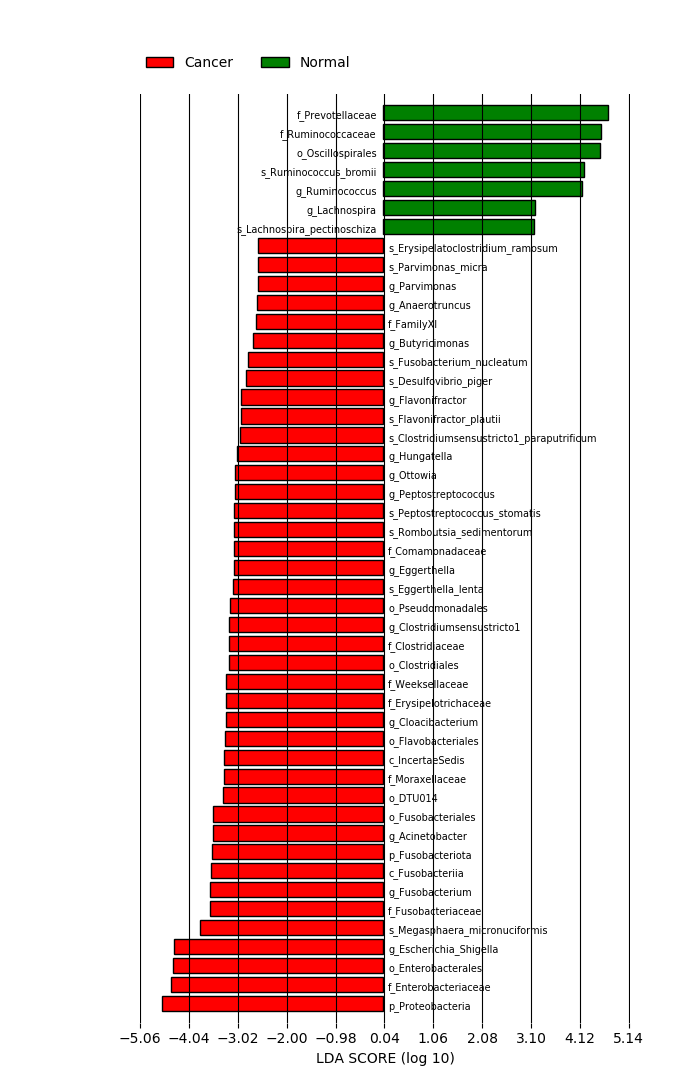
\includegraphics[width=0.8\textwidth,height=\textheight]{images/Fig9.png}

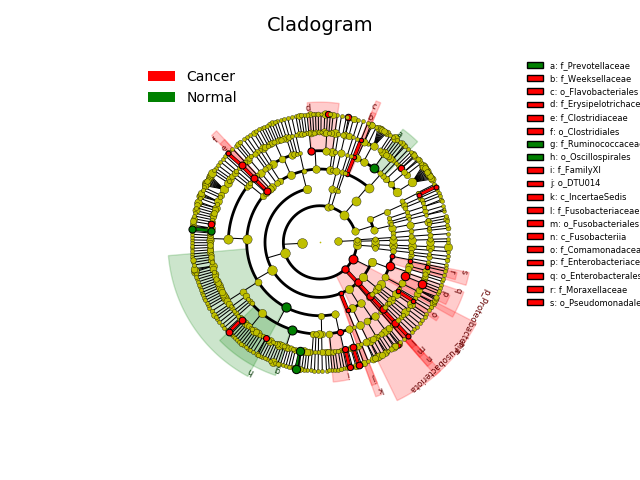
\includegraphics[width=0.8\textwidth,height=\textheight]{images/Fig10.png}

\hypertarget{prelect}{%
\subsection{PreLect}\label{prelect}}

\href{https://github.com/YinchengChen23/PreLectR}{PreLectR} is an R
package implementing the PreLect algorithm, which integrates L1
regularization with an inverted prevalence penalty to select universal
and informative features in sparse data.

It supports four tasks: binary classification, multi-class
classification, regression, and time-to-event analysis.

\(\text{Binary classification} : J(\mathbf{w}) = \text{BCE}(\mathbf{y}, \hat{\mathbf{y}}) + \color{red}{\lambda \sum_j \frac{|\mathbf{w}_j|}{p_j}}\)

\(\text{Regression} : J(\mathbf{w}) = \text{MSE}(\mathbf{y}, \hat{\mathbf{y}}) + \color{red}{\lambda \sum_j \frac{|\mathbf{w}_j|}{p_j}}\)

\(\text{Multi-class classification} : J(\mathbf{w}) = \frac{1}{c} \sum_{l=1}^{c} \left( \text{BCE}(\mathbf{y}_l, \hat{\mathbf{y}}_l) + \color{red}{\lambda \sum_{j=1}^{d}\frac{|\mathbf{w}_{j,l}|}{p_{j,l}}} \right)\)

\(\text{Time-to-event} : J(\mathbf{w}) = h_0(t) \cdot e^{\sum{x_i \cdot w}}+ \color{red}{\lambda \sum_j \frac{|\mathbf{w}_j|}{p_j}}\)

Based on
\href{https://www.nature.com/articles/s41467-021-23821-6}{previous
studies}, we recommend using variance-stabilizing transformation (VST)
for data normalization.

\begin{Shaded}
\begin{Highlighting}[]
\CommentTok{\# Variance Stabilization Transformation}
\FunctionTok{library}\NormalTok{(DESeq2)}
\FunctionTok{library}\NormalTok{(PreLectR)}
\NormalTok{data\_pseudo\_count }\OtherTok{\textless{}{-}}\NormalTok{ data }\SpecialCharTok{+} \DecValTok{1}
\NormalTok{meta}\SpecialCharTok{$}\NormalTok{Class }\OtherTok{\textless{}{-}} \FunctionTok{factor}\NormalTok{(meta}\SpecialCharTok{$}\NormalTok{Class)}

\NormalTok{dds }\OtherTok{\textless{}{-}} \FunctionTok{DESeqDataSetFromMatrix}\NormalTok{(}\AttributeTok{countData =}\NormalTok{ data\_pseudo\_count,}
                              \AttributeTok{colData =}\NormalTok{ meta,}
                              \SpecialCharTok{\textasciitilde{}}\NormalTok{ Class)}

\NormalTok{vst }\OtherTok{\textless{}{-}} \FunctionTok{varianceStabilizingTransformation}\NormalTok{(dds, }\AttributeTok{fitType=}\StringTok{"mean"}\NormalTok{, }\AttributeTok{blind=}\NormalTok{ T)}

\NormalTok{vst\_table }\OtherTok{\textless{}{-}} \FunctionTok{assay}\NormalTok{(vst)}

\CommentTok{\# feature{-}wise z{-}standardization}
\NormalTok{data\_scaled }\OtherTok{\textless{}{-}} \FunctionTok{t}\NormalTok{(}\FunctionTok{scale}\NormalTok{(}\FunctionTok{t}\NormalTok{(}\FunctionTok{as.matrix}\NormalTok{(vst\_table))))}
\end{Highlighting}
\end{Shaded}

We will only use z-standardized table \texttt{data\_scaled} and raw
count table \texttt{data} for the subsequent analyses.

Automatically perform lambda scanning to identify 30 lambda values for
examination.

\begin{Shaded}
\begin{Highlighting}[]
\NormalTok{meta}\SpecialCharTok{$}\NormalTok{Class }\OtherTok{\textless{}{-}} \FunctionTok{factor}\NormalTok{(meta}\SpecialCharTok{$}\NormalTok{Class, }\AttributeTok{levels =} \FunctionTok{c}\NormalTok{(}\StringTok{"Normal"}\NormalTok{, }\StringTok{"Cancer"}\NormalTok{))  }\CommentTok{\# assign "Normal" as control sample}
\NormalTok{lrange }\OtherTok{\textless{}{-}} \FunctionTok{AutoScanning}\NormalTok{(data\_scaled, data, meta}\SpecialCharTok{$}\NormalTok{Class, }\AttributeTok{step =}\DecValTok{30}\NormalTok{)}
\DocumentationTok{\#\#   |                                                                              |                                                                      |   0\%  |                                                                              |=======                                                               |  10\%  |                                                                              |==============                                                        |  20\%  |                                                                              |=====================                                                 |  30\%  |                                                                              |============================                                          |  40\%  |                                                                              |===================================                                   |  50\%  |                                                                              |==========================================                            |  60\%  |                                                                              |=================================================                     |  70\%  |                                                                              |========================================================              |  80\%  |                                                                              |===============================================================       |  90\%  |                                                                              |======================================================================| 100\%}
\FunctionTok{length}\NormalTok{(lrange)}
\DocumentationTok{\#\# [1] 30}
\FunctionTok{exp}\NormalTok{(lrange)}
\DocumentationTok{\#\#  [1] 1.000000e{-}07 1.487352e{-}07 2.212216e{-}07 3.290345e{-}07 4.893901e{-}07}
\DocumentationTok{\#\#  [6] 7.278954e{-}07 1.082637e{-}06 1.610262e{-}06 2.395027e{-}06 3.562248e{-}06}
\DocumentationTok{\#\# [11] 5.298317e{-}06 7.880463e{-}06 1.172102e{-}05 1.743329e{-}05 2.592944e{-}05}
\DocumentationTok{\#\# [16] 3.856620e{-}05 5.736153e{-}05 8.531679e{-}05 1.268961e{-}04 1.887392e{-}04}
\DocumentationTok{\#\# [21] 2.807216e{-}04 4.175319e{-}04 6.210169e{-}04 9.236709e{-}04 1.373824e{-}03}
\DocumentationTok{\#\# [26] 2.043360e{-}03 3.039195e{-}03 4.520354e{-}03 6.723358e{-}03 1.000000e{-}02}

\CommentTok{\# Examining the testing lambda.}
\FunctionTok{dir.create}\NormalTok{(}\StringTok{"\textasciitilde{}/Course/NDMC\_2025/tmp/PreLect\_tmp"}\NormalTok{)}
\NormalTok{output\_path }\OtherTok{\textless{}{-}}\StringTok{"\textasciitilde{}/Course/NDMC\_2025/tmp/PreLect\_tmp"}
\NormalTok{tuning\_res }\OtherTok{\textless{}{-}} \FunctionTok{LambdaTuningParallel}\NormalTok{(data\_scaled, data, meta}\SpecialCharTok{$}\NormalTok{Class, lrange, }\AttributeTok{n\_cores=}\DecValTok{10}\NormalTok{, }\AttributeTok{outpath=}\NormalTok{output\_path)}
\end{Highlighting}
\end{Shaded}

\begin{Shaded}
\begin{Highlighting}[]
\FunctionTok{head}\NormalTok{(tuning\_res}\SpecialCharTok{$}\NormalTok{TuningResult)}
\end{Highlighting}
\end{Shaded}

\begin{verbatim}
##   Feature_number Percentage Prevalence  AUC loss_history error_history
## 1           1051  0.2892926       0.15 0.75 0.0003444818  9.998251e-05
## 2            988  0.2719516       0.15 0.75 0.0003522416  9.997643e-05
## 3            943  0.2595651       0.15 0.75 0.0003449498  9.998842e-05
## 4            805  0.2215800       0.20 0.75 0.0003388232  9.999399e-05
## 5            653  0.1797413       0.25 0.75 0.0003578406  9.999683e-05
## 6            556  0.1530416       0.30 0.75 0.0003616958  9.990256e-05
##     loglmbd
## 1 -16.11810
## 2 -15.72110
## 3 -15.32410
## 4 -14.92710
## 5 -14.53011
## 6 -14.13311
\end{verbatim}

\begin{Shaded}
\begin{Highlighting}[]
\FunctionTok{head}\NormalTok{(tuning\_res}\SpecialCharTok{$}\NormalTok{PvlDistSummary)}
\end{Highlighting}
\end{Shaded}

\begin{verbatim}
##       llmbd max    q3     q2    q1 min
## 1 -16.11810   1 0.300 0.1375 0.075   0
## 2 -15.72110   1 0.325 0.1500 0.100   0
## 3 -15.32410   1 0.325 0.1500 0.100   0
## 4 -14.92710   1 0.375 0.2000 0.100   0
## 5 -14.53011   1 0.450 0.2500 0.125   0
## 6 -14.13311   1 0.500 0.3000 0.175   0
\end{verbatim}

Determine the optimal lambda by partitioning tree.

\begin{Shaded}
\begin{Highlighting}[]
\NormalTok{lmbd\_picking }\OtherTok{\textless{}{-}} \FunctionTok{LambdaDecision}\NormalTok{(tuning\_res}\SpecialCharTok{$}\NormalTok{TuningResult, tuning\_res}\SpecialCharTok{$}\NormalTok{PvlDistSummary, }\AttributeTok{maxdepth=}\DecValTok{5}\NormalTok{, }\AttributeTok{minbucket=}\DecValTok{3}\NormalTok{)}

\NormalTok{lmbd\_picking}\SpecialCharTok{$}\NormalTok{selected\_lmbd\_plot}\SpecialCharTok{/}\NormalTok{lmbd\_picking}\SpecialCharTok{$}\NormalTok{pvl\_plot}
\end{Highlighting}
\end{Shaded}

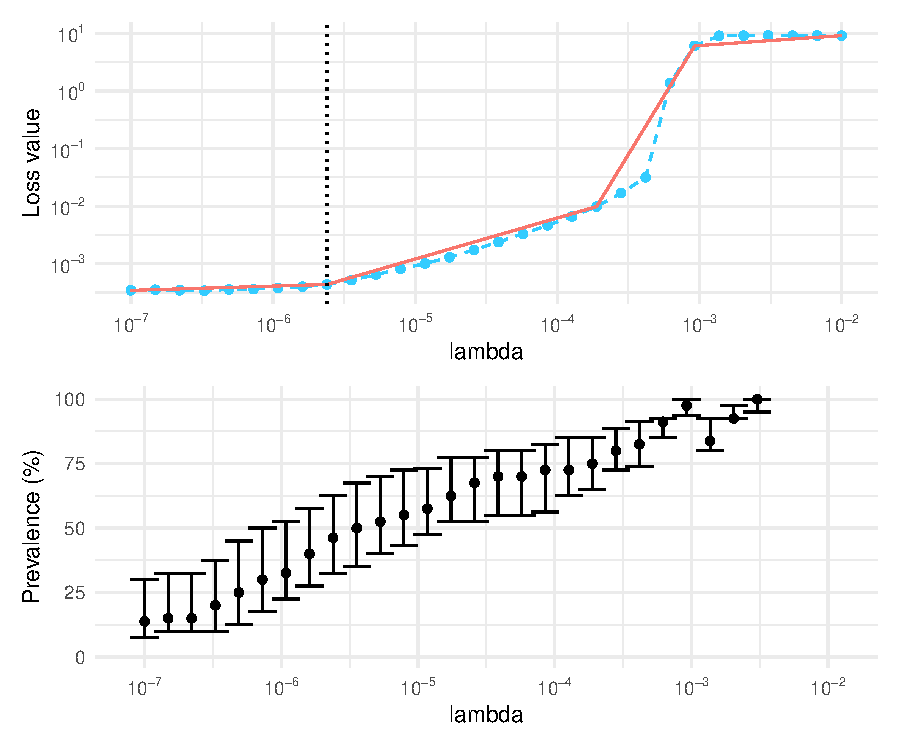
\includegraphics{workshop_files/figure-latex/unnamed-chunk-46-1.pdf}

\begin{Shaded}
\begin{Highlighting}[]

\FunctionTok{print}\NormalTok{(lmbd\_picking}\SpecialCharTok{$}\NormalTok{opt\_lmbd)}
\DocumentationTok{\#\# [1] 2.395027e{-}06}
\end{Highlighting}
\end{Shaded}

PreLect execution and get the property for each feature

\begin{Shaded}
\begin{Highlighting}[]
\CommentTok{\# We strongly suggest using 100000 for max\_iter to achieve more accurate results.}
\NormalTok{s}\OtherTok{=}\FunctionTok{Sys.time}\NormalTok{()}
\NormalTok{prevalence }\OtherTok{\textless{}{-}} \FunctionTok{GetPrevalence}\NormalTok{(data)}
\NormalTok{PreLect\_out }\OtherTok{\textless{}{-}} \FunctionTok{PreLect}\NormalTok{(data\_scaled, prevalence, meta}\SpecialCharTok{$}\NormalTok{Class, }\AttributeTok{lambda=}\NormalTok{lmbd\_picking}\SpecialCharTok{$}\NormalTok{opt\_lmbd, }\AttributeTok{max\_iter =} \DecValTok{100000}\NormalTok{)}
\FunctionTok{print}\NormalTok{(}\FunctionTok{Sys.time}\NormalTok{()}\SpecialCharTok{{-}}\NormalTok{s)}
\DocumentationTok{\#\# Time difference of 3.083079 secs}


\NormalTok{featpropt }\OtherTok{\textless{}{-}} \FunctionTok{FeatureProperty}\NormalTok{(data, meta}\SpecialCharTok{$}\NormalTok{Class, PreLect\_out, }\AttributeTok{task=}\StringTok{"classification"}\NormalTok{)}

\FunctionTok{print}\NormalTok{(}\FunctionTok{paste}\NormalTok{(}\FunctionTok{nrow}\NormalTok{(featpropt[featpropt}\SpecialCharTok{$}\NormalTok{selected }\SpecialCharTok{==} \StringTok{\textquotesingle{}Selected\textquotesingle{}}\NormalTok{, ]), }\StringTok{\textquotesingle{}features were selected\textquotesingle{}}\NormalTok{))}
\DocumentationTok{\#\# [1] "336 features were selected"}

\FunctionTok{print}\NormalTok{(}\FunctionTok{paste}\NormalTok{(}\StringTok{\textquotesingle{}median of prevalence :\textquotesingle{}}\NormalTok{, }\FunctionTok{median}\NormalTok{(featpropt}\SpecialCharTok{$}\NormalTok{prevalence[featpropt}\SpecialCharTok{$}\NormalTok{selected }\SpecialCharTok{==} \StringTok{\textquotesingle{}Selected\textquotesingle{}}\NormalTok{])))}
\DocumentationTok{\#\# [1] "median of prevalence : 0.425"}

\FunctionTok{write.table}\NormalTok{(featpropt, }\StringTok{"\textasciitilde{}/Course/NDMC\_2025/tmp/PreLect\_tmp/feature\_propt.txt"}\NormalTok{, }\AttributeTok{quote=}\ConstantTok{FALSE}\NormalTok{, }\AttributeTok{sep=}\StringTok{"}\SpecialCharTok{\textbackslash{}t}\StringTok{"}\NormalTok{)}
\FunctionTok{head}\NormalTok{(featpropt)}
\DocumentationTok{\#\#         FeatName        coef tendency selected meanAbundance   variance}
\DocumentationTok{\#\# ASV0001  ASV0001  0.54988067   Cancer Selected    0.04150302  117734960}
\DocumentationTok{\#\# ASV0002  ASV0002 {-}0.42573824   Normal Selected    0.03167390   64237504}
\DocumentationTok{\#\# ASV0003  ASV0003  0.00000000     \textless{}NA\textgreater{}   Others    0.01213962 1555924984}
\DocumentationTok{\#\# ASV0004  ASV0004 {-}0.33145665   Normal Selected    0.03201389  288009324}
\DocumentationTok{\#\# ASV0005  ASV0005 {-}0.32683697   Normal Selected    0.02903994   41768447}
\DocumentationTok{\#\# ASV0006  ASV0006 {-}0.03458693   Normal Selected    0.02485074   72058376}
\DocumentationTok{\#\#         prevalence prevalence\_case prevalence\_control      logFC}
\DocumentationTok{\#\# ASV0001      1.000            1.00               1.00  1.4998663}
\DocumentationTok{\#\# ASV0002      0.975            0.95               1.00 {-}0.6884894}
\DocumentationTok{\#\# ASV0003      0.100            0.05               0.15 11.0217666}
\DocumentationTok{\#\# ASV0004      0.650            0.60               0.70 {-}2.6154169}
\DocumentationTok{\#\# ASV0005      0.875            0.80               0.95  0.6372900}
\DocumentationTok{\#\# ASV0006      0.925            0.90               0.95 {-}0.1468191}
\end{Highlighting}
\end{Shaded}

Selection profile visualization and evaluation

\begin{Shaded}
\begin{Highlighting}[]
\FunctionTok{ggplot}\NormalTok{(featpropt, }\FunctionTok{aes}\NormalTok{(}\AttributeTok{x =}\NormalTok{ prevalence, }\AttributeTok{y =}\NormalTok{ meanAbundance, }\AttributeTok{color=}\NormalTok{selected)) }\SpecialCharTok{+} \FunctionTok{geom\_point}\NormalTok{() }\SpecialCharTok{+}
  \FunctionTok{scale\_color\_manual}\NormalTok{(}\AttributeTok{values =} \FunctionTok{c}\NormalTok{(}\StringTok{\textquotesingle{}Selected\textquotesingle{}}\OtherTok{=}\StringTok{\textquotesingle{}red\textquotesingle{}}\NormalTok{, }\StringTok{\textquotesingle{}Others\textquotesingle{}}\OtherTok{=}\StringTok{\textquotesingle{}\#AAAAAA\textquotesingle{}}\NormalTok{)) }\SpecialCharTok{+} 
  \FunctionTok{scale\_y\_log10}\NormalTok{(}\AttributeTok{breaks =} \FunctionTok{trans\_breaks}\NormalTok{(}\StringTok{"log10"}\NormalTok{, }\ControlFlowTok{function}\NormalTok{(x) }\DecValTok{10}\SpecialCharTok{\^{}}\NormalTok{x),}
                \AttributeTok{labels =} \FunctionTok{trans\_format}\NormalTok{(}\StringTok{"log10"}\NormalTok{, }\FunctionTok{math\_format}\NormalTok{(}\DecValTok{10}\SpecialCharTok{\^{}}\NormalTok{.x))) }\SpecialCharTok{+}
  \FunctionTok{theme\_bw}\NormalTok{()}\SpecialCharTok{+} \FunctionTok{theme}\NormalTok{(}\AttributeTok{panel.background =} \FunctionTok{element\_rect}\NormalTok{(}\AttributeTok{fill =} \StringTok{"white"}\NormalTok{, }\AttributeTok{colour =} \StringTok{"white"}\NormalTok{))}
\end{Highlighting}
\end{Shaded}

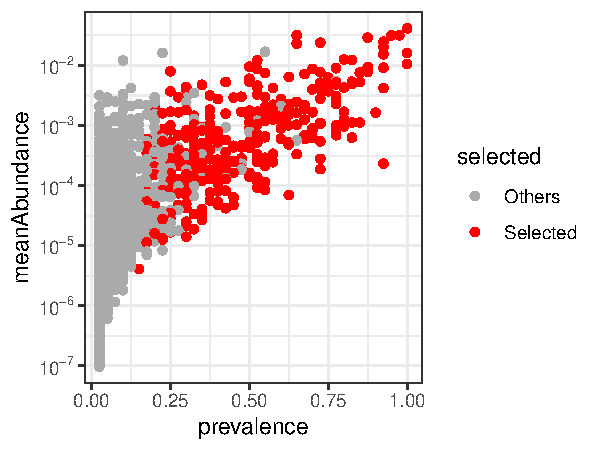
\includegraphics{workshop_files/figure-latex/unnamed-chunk-48-1.pdf}

\begin{Shaded}
\begin{Highlighting}[]

\FunctionTok{ggplot}\NormalTok{(featpropt, }\FunctionTok{aes}\NormalTok{(}\AttributeTok{x =}\NormalTok{ logFC, }\AttributeTok{y =}\NormalTok{ prevalence, }\AttributeTok{color=}\NormalTok{selected)) }\SpecialCharTok{+} \FunctionTok{geom\_point}\NormalTok{() }\SpecialCharTok{+}
  \FunctionTok{scale\_color\_manual}\NormalTok{(}\AttributeTok{values =} \FunctionTok{c}\NormalTok{(}\StringTok{\textquotesingle{}Selected\textquotesingle{}}\OtherTok{=}\StringTok{\textquotesingle{}red\textquotesingle{}}\NormalTok{, }\StringTok{\textquotesingle{}Others\textquotesingle{}}\OtherTok{=}\StringTok{\textquotesingle{}\#AAAAAA\textquotesingle{}}\NormalTok{)) }\SpecialCharTok{+} 
  \FunctionTok{theme\_bw}\NormalTok{()}\SpecialCharTok{+} \FunctionTok{theme}\NormalTok{(}\AttributeTok{panel.background =} \FunctionTok{element\_rect}\NormalTok{(}\AttributeTok{fill =} \StringTok{"white"}\NormalTok{, }\AttributeTok{colour =} \StringTok{"white"}\NormalTok{))}
\end{Highlighting}
\end{Shaded}

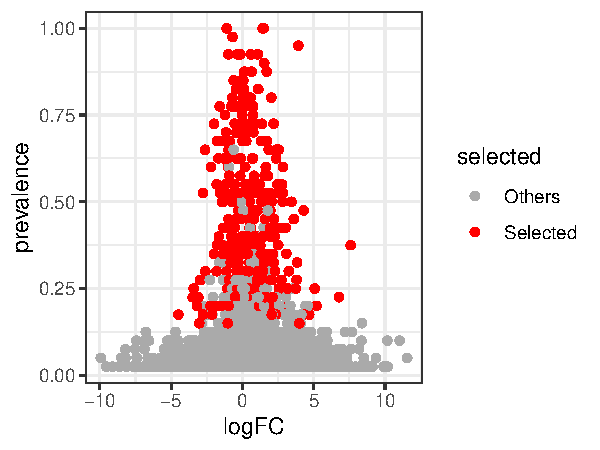
\includegraphics{workshop_files/figure-latex/unnamed-chunk-48-2.pdf}

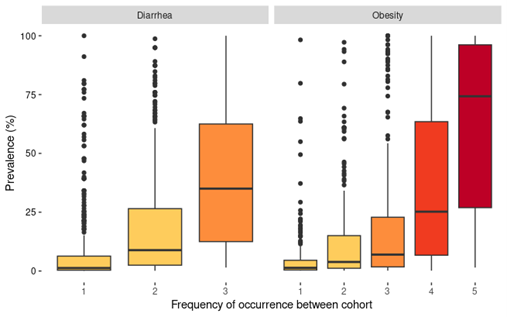
\includegraphics[width=0.8\textwidth,height=\textheight]{images/Fig19.png}

We observed that features present in multiple datasets tend to have
higher prevalence within those datasets. This finding suggests that
features with higher prevalence in one dataset are more likely to be
universal across different datasets.

\begin{Shaded}
\begin{Highlighting}[]
\NormalTok{y }\OtherTok{\textless{}{-}} \FunctionTok{ifelse}\NormalTok{(meta}\SpecialCharTok{$}\NormalTok{Class }\SpecialCharTok{==} \StringTok{"Cancer"}\NormalTok{, }\DecValTok{1}\NormalTok{, }\DecValTok{0}\NormalTok{) }

\NormalTok{split   }\OtherTok{\textless{}{-}} \FunctionTok{TrainTextSplit}\NormalTok{(y, }\AttributeTok{ratio =} \FloatTok{0.8}\NormalTok{)}
\NormalTok{X\_train }\OtherTok{\textless{}{-}}\NormalTok{ data\_scaled[, split}\SpecialCharTok{$}\NormalTok{train\_idx]}
\NormalTok{X\_test  }\OtherTok{\textless{}{-}}\NormalTok{ data\_scaled[, split}\SpecialCharTok{$}\NormalTok{test\_idx]}
\NormalTok{y\_train }\OtherTok{\textless{}{-}}\NormalTok{ y[split}\SpecialCharTok{$}\NormalTok{train\_idx]}
\NormalTok{y\_test  }\OtherTok{\textless{}{-}}\NormalTok{ y[split}\SpecialCharTok{$}\NormalTok{test\_idx]}

\NormalTok{perf }\OtherTok{\textless{}{-}} \FunctionTok{evaluation}\NormalTok{(X\_train, y\_train, X\_test, y\_test, featpropt}\SpecialCharTok{$}\NormalTok{coef, }\AttributeTok{task=}\StringTok{\textquotesingle{}classification\textquotesingle{}}\NormalTok{)}
\NormalTok{perf}
\DocumentationTok{\#\# $AUC}
\DocumentationTok{\#\# [1] 0.875}
\end{Highlighting}
\end{Shaded}

\begin{Shaded}
\begin{Highlighting}[]
\NormalTok{result }\OtherTok{\textless{}{-}} \FunctionTok{TaxaProperty}\NormalTok{(featpropt, taxa, }\StringTok{"Family"}\NormalTok{,  }\AttributeTok{pvl\_filter =} \FloatTok{0.5}\NormalTok{)}

\NormalTok{mycolor }\OtherTok{\textless{}{-}} \FunctionTok{c}\NormalTok{(}\StringTok{"Normal"} \OtherTok{=} \StringTok{"\#FFCC22"}\NormalTok{, }\StringTok{"Cancer"} \OtherTok{=} \StringTok{"\#EE7700"}\NormalTok{)}
\NormalTok{result}\SpecialCharTok{$}\NormalTok{effectSizePlot }\SpecialCharTok{+} \FunctionTok{scale\_fill\_manual}\NormalTok{(}\AttributeTok{values =}\NormalTok{ mycolor) }\SpecialCharTok{+}
   \FunctionTok{geom\_hline}\NormalTok{(}\AttributeTok{yintercept =} \DecValTok{0}\NormalTok{, }\AttributeTok{color=}\StringTok{\textquotesingle{}black\textquotesingle{}}\NormalTok{, }\AttributeTok{linetype=}\StringTok{\textquotesingle{}dashed\textquotesingle{}}\NormalTok{)}
\end{Highlighting}
\end{Shaded}

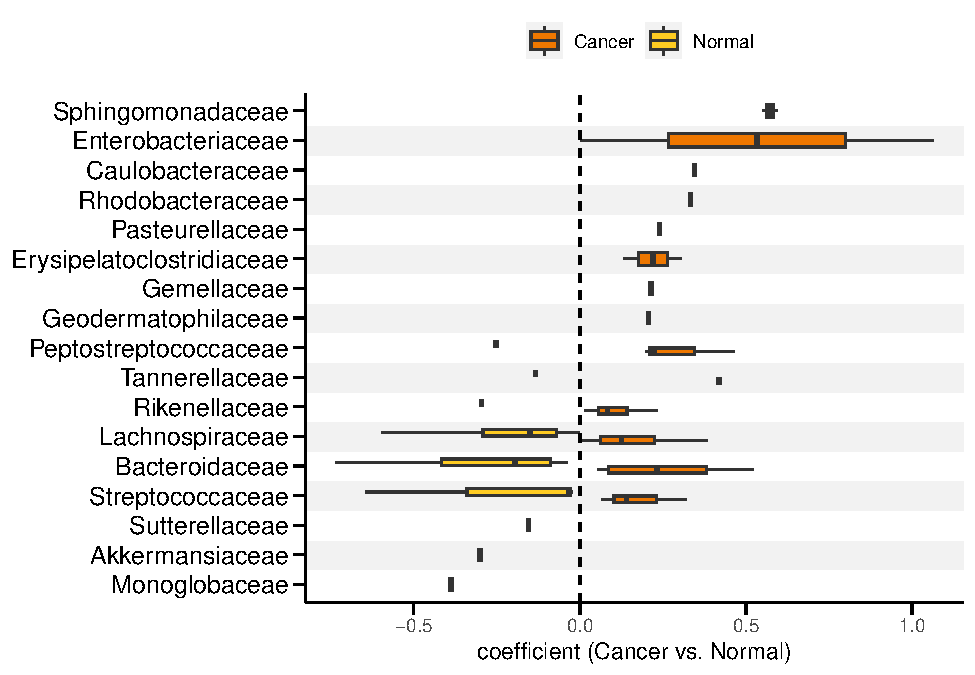
\includegraphics{workshop_files/figure-latex/unnamed-chunk-50-1.pdf}

\begin{Shaded}
\begin{Highlighting}[]
\FunctionTok{head}\NormalTok{(result}\SpecialCharTok{$}\NormalTok{selectedInfo)}
\DocumentationTok{\#\#         FeatName       coef tendency selected meanAbundance  variance}
\DocumentationTok{\#\# ASV0001  ASV0001  0.5498807   Cancer Selected    0.04150302 117734960}
\DocumentationTok{\#\# ASV0002  ASV0002 {-}0.4257382   Normal Selected    0.03167390  64237504}
\DocumentationTok{\#\# ASV0005  ASV0005 {-}0.3268370   Normal Selected    0.02903994  41768447}
\DocumentationTok{\#\# ASV0007  ASV0007  1.0654049   Cancer Selected    0.03158703 178336011}
\DocumentationTok{\#\# ASV0008  ASV0008 {-}0.3002699   Normal Selected    0.02299001 312317781}
\DocumentationTok{\#\# ASV0009  ASV0009 {-}0.4994069   Normal Selected    0.02042962  45214122}
\DocumentationTok{\#\#         prevalence prevalence\_case prevalence\_control      logFC}
\DocumentationTok{\#\# ASV0001      1.000            1.00               1.00  1.4998663}
\DocumentationTok{\#\# ASV0002      0.975            0.95               1.00 {-}0.6884894}
\DocumentationTok{\#\# ASV0005      0.875            0.80               0.95  0.6372900}
\DocumentationTok{\#\# ASV0007      0.950            1.00               0.90  3.9252053}
\DocumentationTok{\#\# ASV0008      0.650            0.65               0.65  1.8688587}
\DocumentationTok{\#\# ASV0009      0.925            0.85               1.00  0.5991814}
\DocumentationTok{\#\#                       taxa}
\DocumentationTok{\#\# ASV0001  Sphingomonadaceae}
\DocumentationTok{\#\# ASV0002    Lachnospiraceae}
\DocumentationTok{\#\# ASV0005     Bacteroidaceae}
\DocumentationTok{\#\# ASV0007 Enterobacteriaceae}
\DocumentationTok{\#\# ASV0008    Akkermansiaceae}
\DocumentationTok{\#\# ASV0009    Lachnospiraceae}
\end{Highlighting}
\end{Shaded}

\hypertarget{basal-feature-visualization}{%
\subsection{Basal feature
visualization}\label{basal-feature-visualization}}

we use edgeR to demonstrate the several plots.

\begin{Shaded}
\begin{Highlighting}[]
\FunctionTok{library}\NormalTok{(edgeR)}

\NormalTok{ASV }\OtherTok{\textless{}{-}}\NormalTok{ phyloseq}\SpecialCharTok{::}\FunctionTok{otu\_table}\NormalTok{(data, }\AttributeTok{taxa\_are\_rows =}\NormalTok{ T)}
\NormalTok{sampledata }\OtherTok{\textless{}{-}}\NormalTok{ phyloseq}\SpecialCharTok{::}\FunctionTok{sample\_data}\NormalTok{(meta, }\AttributeTok{errorIfNULL =}\NormalTok{ T)}
\NormalTok{phylo }\OtherTok{\textless{}{-}}\NormalTok{ phyloseq}\SpecialCharTok{::}\FunctionTok{merge\_phyloseq}\NormalTok{(ASV, sampledata)}
\NormalTok{test }\OtherTok{\textless{}{-}} \FunctionTok{phyloseq\_to\_edgeR}\NormalTok{(}\AttributeTok{physeq =}\NormalTok{ phylo, }\AttributeTok{group =} \StringTok{"Class"}\NormalTok{)}
\NormalTok{et }\OtherTok{=} \FunctionTok{exactTest}\NormalTok{(test)}
\NormalTok{out }\OtherTok{=} \FunctionTok{topTags}\NormalTok{(et, }\AttributeTok{n=}\FunctionTok{nrow}\NormalTok{(test}\SpecialCharTok{$}\NormalTok{table), }\AttributeTok{adjust.method=}\StringTok{"BH"}\NormalTok{, }\AttributeTok{sort.by=}\StringTok{"PValue"}\NormalTok{)}
\NormalTok{edgeR\_result }\OtherTok{\textless{}{-}}\NormalTok{ out}\SpecialCharTok{@}\NormalTok{.Data[[}\DecValTok{1}\NormalTok{]]}
\NormalTok{edgeR\_selected }\OtherTok{\textless{}{-}}\NormalTok{ edgeR\_result[edgeR\_result}\SpecialCharTok{$}\NormalTok{FDR }\SpecialCharTok{\textless{}} \FloatTok{0.05}\NormalTok{,]}

\NormalTok{et }\OtherTok{=} \FunctionTok{exactTest}\NormalTok{(test)}
\NormalTok{et }\OtherTok{=}\NormalTok{ et}\SpecialCharTok{$}\NormalTok{table}
\NormalTok{et}\SpecialCharTok{$}\NormalTok{select }\OtherTok{\textless{}{-}} \StringTok{"drop"}
\NormalTok{et}\SpecialCharTok{$}\NormalTok{select[}\FunctionTok{rownames}\NormalTok{(et) }\SpecialCharTok{\%in\%} \FunctionTok{rownames}\NormalTok{(edgeR\_selected)] }\OtherTok{=} \StringTok{"selected"}

\NormalTok{data\_freq }\OtherTok{\textless{}{-}}\NormalTok{ data}
\ControlFlowTok{for}\NormalTok{(i }\ControlFlowTok{in} \DecValTok{1}\SpecialCharTok{:}\FunctionTok{ncol}\NormalTok{(data\_freq))\{}
\NormalTok{  data\_freq[,i] }\OtherTok{\textless{}{-}}\NormalTok{ data\_freq[,i]}\SpecialCharTok{/}\FunctionTok{colSums}\NormalTok{(data\_freq)[i]}
\NormalTok{\}}


\NormalTok{get\_pvl }\OtherTok{\textless{}{-}} \ControlFlowTok{function}\NormalTok{(m)\{}
\NormalTok{  m\_ }\OtherTok{\textless{}{-}}\NormalTok{ m}
\NormalTok{  m\_[m\_ }\SpecialCharTok{\textgreater{}} \DecValTok{0}\NormalTok{] }\OtherTok{=} \DecValTok{1}
\NormalTok{  m\_ }\OtherTok{\textless{}{-}} \FunctionTok{as.matrix}\NormalTok{(m\_)}
  \FunctionTok{return}\NormalTok{(}\FunctionTok{as.numeric}\NormalTok{(}\FunctionTok{rowSums}\NormalTok{(m\_)}\SpecialCharTok{/}\FunctionTok{ncol}\NormalTok{(m\_)))}
\NormalTok{\}}

\NormalTok{variance }\OtherTok{\textless{}{-}} \FunctionTok{c}\NormalTok{()}
\ControlFlowTok{for}\NormalTok{(i }\ControlFlowTok{in} \DecValTok{1}\SpecialCharTok{:}\FunctionTok{nrow}\NormalTok{(data\_freq))\{}
\NormalTok{  variance }\OtherTok{\textless{}{-}} \FunctionTok{c}\NormalTok{(variance, }\FunctionTok{log}\NormalTok{(}\FunctionTok{sd}\NormalTok{(data\_freq[i,])}\SpecialCharTok{**}\DecValTok{2}\NormalTok{))}
\NormalTok{\}}

\NormalTok{et}\SpecialCharTok{$}\NormalTok{variation }\OtherTok{\textless{}{-}}\NormalTok{ variance}
\NormalTok{et}\SpecialCharTok{$}\NormalTok{prevalence }\OtherTok{\textless{}{-}} \FunctionTok{get\_pvl}\NormalTok{(data)}
\NormalTok{et}\SpecialCharTok{$}\NormalTok{neglog2p }\OtherTok{\textless{}{-}} \SpecialCharTok{{-}}\FunctionTok{log}\NormalTok{(et}\SpecialCharTok{$}\NormalTok{PValue,}\DecValTok{2}\NormalTok{)}
\NormalTok{et}\SpecialCharTok{$}\NormalTok{select }\OtherTok{\textless{}{-}} \FunctionTok{factor}\NormalTok{(et}\SpecialCharTok{$}\NormalTok{select, }\AttributeTok{levels =} \FunctionTok{c}\NormalTok{(}\StringTok{\textquotesingle{}selected\textquotesingle{}}\NormalTok{,}\StringTok{\textquotesingle{}drop\textquotesingle{}}\NormalTok{))}

\FunctionTok{ggplot}\NormalTok{(et, }\FunctionTok{aes}\NormalTok{(}\AttributeTok{x =}\NormalTok{ logFC, }\AttributeTok{y =}\NormalTok{ neglog2p, }\AttributeTok{color =}\NormalTok{ select)) }\SpecialCharTok{+} \FunctionTok{geom\_point}\NormalTok{() }\SpecialCharTok{+}
  \FunctionTok{xlab}\NormalTok{(}\StringTok{\textquotesingle{}log(FC) Cancer vs. Normal\textquotesingle{}}\NormalTok{) }\SpecialCharTok{+} \FunctionTok{ylab}\NormalTok{(}\StringTok{\textquotesingle{}{-}log2(p value)\textquotesingle{}}\NormalTok{) }\SpecialCharTok{+} 
  \FunctionTok{scale\_color\_brewer}\NormalTok{(}\AttributeTok{palette =} \StringTok{\textquotesingle{}Set1\textquotesingle{}}\NormalTok{) }\SpecialCharTok{+} \FunctionTok{theme}\NormalTok{(}\AttributeTok{axis.line =} \FunctionTok{element\_line}\NormalTok{(}\AttributeTok{linetype =} \DecValTok{1}\NormalTok{,}\AttributeTok{colour =} \StringTok{\textquotesingle{}black\textquotesingle{}}\NormalTok{),}
        \AttributeTok{panel.background =} \FunctionTok{element\_rect}\NormalTok{(}\FunctionTok{I}\NormalTok{(}\DecValTok{0}\NormalTok{)),}
        \AttributeTok{panel.grid.major =} \FunctionTok{element\_line}\NormalTok{(}\AttributeTok{colour =} \ConstantTok{NA}\NormalTok{),}
        \AttributeTok{panel.grid.minor =} \FunctionTok{element\_line}\NormalTok{(}\AttributeTok{colour =} \ConstantTok{NA}\NormalTok{))}
\end{Highlighting}
\end{Shaded}

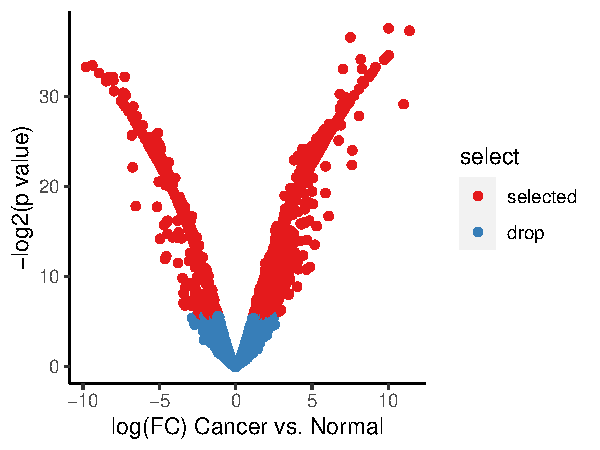
\includegraphics{workshop_files/figure-latex/unnamed-chunk-51-1.pdf}

\begin{Shaded}
\begin{Highlighting}[]

\FunctionTok{ggplot}\NormalTok{(et, }\FunctionTok{aes}\NormalTok{(}\AttributeTok{x =}\NormalTok{ logCPM, }\AttributeTok{y =}\NormalTok{ logFC, }\AttributeTok{color =}\NormalTok{ select)) }\SpecialCharTok{+} \FunctionTok{geom\_point}\NormalTok{() }\SpecialCharTok{+}
  \FunctionTok{xlab}\NormalTok{(}\StringTok{\textquotesingle{}Relative abundance (logCPM)\textquotesingle{}}\NormalTok{) }\SpecialCharTok{+} \FunctionTok{ylab}\NormalTok{(}\StringTok{\textquotesingle{}log(FC) Cancer vs. Normal\textquotesingle{}}\NormalTok{) }\SpecialCharTok{+} 
  \FunctionTok{scale\_color\_brewer}\NormalTok{(}\AttributeTok{palette =} \StringTok{\textquotesingle{}Set1\textquotesingle{}}\NormalTok{) }\SpecialCharTok{+}
  \FunctionTok{theme}\NormalTok{(}\AttributeTok{axis.line =} \FunctionTok{element\_line}\NormalTok{(}\AttributeTok{linetype =} \DecValTok{1}\NormalTok{,}\AttributeTok{colour =} \StringTok{\textquotesingle{}black\textquotesingle{}}\NormalTok{),}
        \AttributeTok{panel.background =} \FunctionTok{element\_rect}\NormalTok{(}\FunctionTok{I}\NormalTok{(}\DecValTok{0}\NormalTok{)),}
        \AttributeTok{panel.grid.major =} \FunctionTok{element\_line}\NormalTok{(}\AttributeTok{colour =} \ConstantTok{NA}\NormalTok{),}
        \AttributeTok{panel.grid.minor =} \FunctionTok{element\_line}\NormalTok{(}\AttributeTok{colour =} \ConstantTok{NA}\NormalTok{))}
\end{Highlighting}
\end{Shaded}

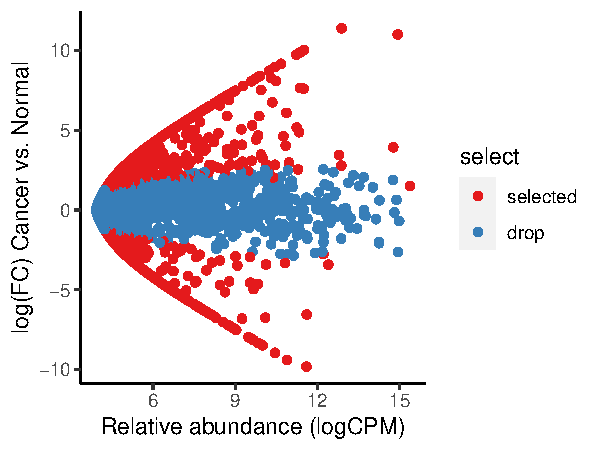
\includegraphics{workshop_files/figure-latex/unnamed-chunk-51-2.pdf}

\begin{Shaded}
\begin{Highlighting}[]

\FunctionTok{ggplot}\NormalTok{(et, }\FunctionTok{aes}\NormalTok{(}\AttributeTok{x =}\NormalTok{ prevalence, }\AttributeTok{y =}\NormalTok{ logFC, }\AttributeTok{color =}\NormalTok{ select)) }\SpecialCharTok{+} \FunctionTok{geom\_point}\NormalTok{() }\SpecialCharTok{+}
  \FunctionTok{xlab}\NormalTok{(}\StringTok{\textquotesingle{}Prevalence\textquotesingle{}}\NormalTok{) }\SpecialCharTok{+} \FunctionTok{ylab}\NormalTok{(}\StringTok{\textquotesingle{}log(FC) Cancer vs. Normal\textquotesingle{}}\NormalTok{) }\SpecialCharTok{+} 
  \FunctionTok{scale\_color\_brewer}\NormalTok{(}\AttributeTok{palette =} \StringTok{\textquotesingle{}Set1\textquotesingle{}}\NormalTok{) }\SpecialCharTok{+}
  \FunctionTok{theme}\NormalTok{(}\AttributeTok{axis.line =} \FunctionTok{element\_line}\NormalTok{(}\AttributeTok{linetype =} \DecValTok{1}\NormalTok{,}\AttributeTok{colour =} \StringTok{\textquotesingle{}black\textquotesingle{}}\NormalTok{),}
        \AttributeTok{panel.background =} \FunctionTok{element\_rect}\NormalTok{(}\FunctionTok{I}\NormalTok{(}\DecValTok{0}\NormalTok{)),}
        \AttributeTok{panel.grid.major =} \FunctionTok{element\_line}\NormalTok{(}\AttributeTok{colour =} \ConstantTok{NA}\NormalTok{),}
        \AttributeTok{panel.grid.minor =} \FunctionTok{element\_line}\NormalTok{(}\AttributeTok{colour =} \ConstantTok{NA}\NormalTok{))}
\end{Highlighting}
\end{Shaded}

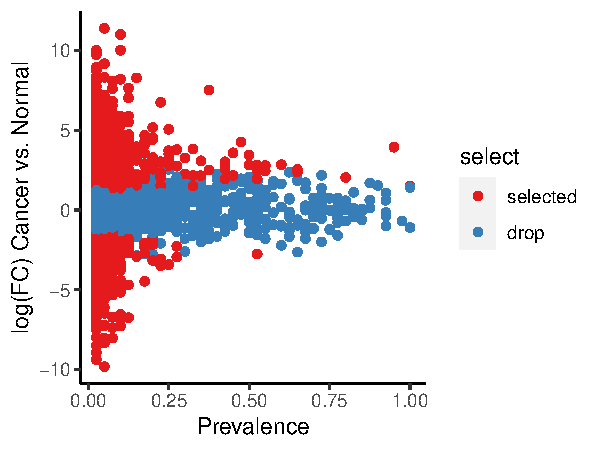
\includegraphics{workshop_files/figure-latex/unnamed-chunk-51-3.pdf}

\begin{Shaded}
\begin{Highlighting}[]

\FunctionTok{ggplot}\NormalTok{(et, }\FunctionTok{aes}\NormalTok{(}\AttributeTok{x =}\NormalTok{ prevalence, }\AttributeTok{y =}\NormalTok{ logCPM, }\AttributeTok{color =}\NormalTok{ select)) }\SpecialCharTok{+} \FunctionTok{geom\_point}\NormalTok{() }\SpecialCharTok{+}
  \FunctionTok{xlab}\NormalTok{(}\StringTok{\textquotesingle{}Prevalence\textquotesingle{}}\NormalTok{) }\SpecialCharTok{+} \FunctionTok{ylab}\NormalTok{(}\StringTok{\textquotesingle{}Relative abundance (logCPM)\textquotesingle{}}\NormalTok{) }\SpecialCharTok{+} 
  \FunctionTok{scale\_color\_brewer}\NormalTok{(}\AttributeTok{palette =} \StringTok{\textquotesingle{}Set1\textquotesingle{}}\NormalTok{) }\SpecialCharTok{+}
  \FunctionTok{theme}\NormalTok{(}\AttributeTok{axis.line =} \FunctionTok{element\_line}\NormalTok{(}\AttributeTok{linetype =} \DecValTok{1}\NormalTok{,}\AttributeTok{colour =} \StringTok{\textquotesingle{}black\textquotesingle{}}\NormalTok{),}
        \AttributeTok{panel.background =} \FunctionTok{element\_rect}\NormalTok{(}\FunctionTok{I}\NormalTok{(}\DecValTok{0}\NormalTok{)),}
        \AttributeTok{panel.grid.major =} \FunctionTok{element\_line}\NormalTok{(}\AttributeTok{colour =} \ConstantTok{NA}\NormalTok{),}
        \AttributeTok{panel.grid.minor =} \FunctionTok{element\_line}\NormalTok{(}\AttributeTok{colour =} \ConstantTok{NA}\NormalTok{))}
\end{Highlighting}
\end{Shaded}

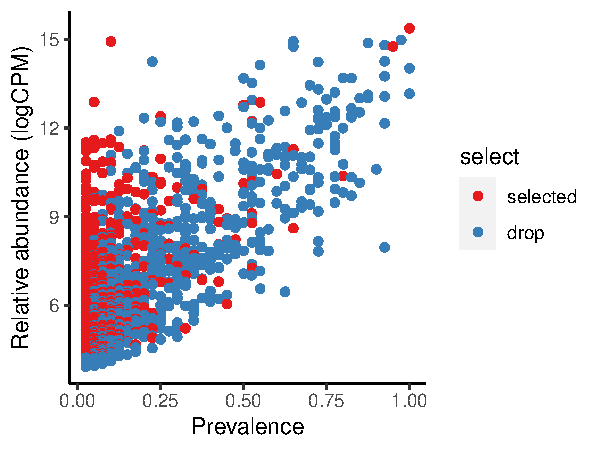
\includegraphics{workshop_files/figure-latex/unnamed-chunk-51-4.pdf}

\begin{Shaded}
\begin{Highlighting}[]

\FunctionTok{ggplot}\NormalTok{(et, }\FunctionTok{aes}\NormalTok{(}\AttributeTok{x =}\NormalTok{ logCPM, }\AttributeTok{y =}\NormalTok{ variance, }\AttributeTok{color =}\NormalTok{ select)) }\SpecialCharTok{+} \FunctionTok{geom\_point}\NormalTok{() }\SpecialCharTok{+}
  \FunctionTok{xlab}\NormalTok{(}\StringTok{\textquotesingle{}Relative abundance (logCPM)\textquotesingle{}}\NormalTok{) }\SpecialCharTok{+} \FunctionTok{ylab}\NormalTok{(}\StringTok{\textquotesingle{}log(variance)\textquotesingle{}}\NormalTok{) }\SpecialCharTok{+} 
  \FunctionTok{scale\_color\_brewer}\NormalTok{(}\AttributeTok{palette =} \StringTok{\textquotesingle{}Set1\textquotesingle{}}\NormalTok{) }\SpecialCharTok{+}
  \FunctionTok{theme}\NormalTok{(}\AttributeTok{axis.line =} \FunctionTok{element\_line}\NormalTok{(}\AttributeTok{linetype =} \DecValTok{1}\NormalTok{,}\AttributeTok{colour =} \StringTok{\textquotesingle{}black\textquotesingle{}}\NormalTok{),}
        \AttributeTok{panel.background =} \FunctionTok{element\_rect}\NormalTok{(}\FunctionTok{I}\NormalTok{(}\DecValTok{0}\NormalTok{)),}
        \AttributeTok{panel.grid.major =} \FunctionTok{element\_line}\NormalTok{(}\AttributeTok{colour =} \ConstantTok{NA}\NormalTok{),}
        \AttributeTok{panel.grid.minor =} \FunctionTok{element\_line}\NormalTok{(}\AttributeTok{colour =} \ConstantTok{NA}\NormalTok{))}
\end{Highlighting}
\end{Shaded}

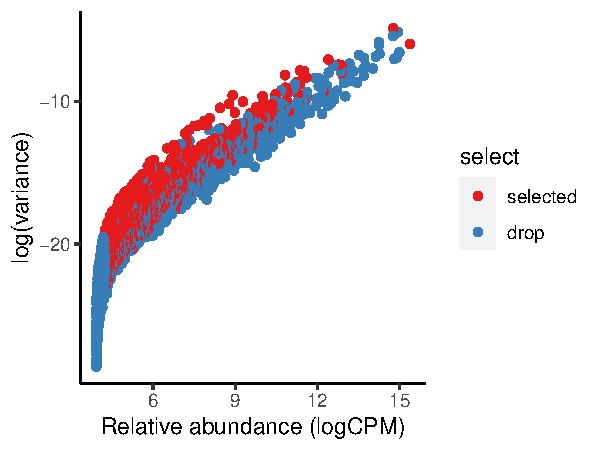
\includegraphics{workshop_files/figure-latex/unnamed-chunk-51-5.pdf}

\begin{Shaded}
\begin{Highlighting}[]

\FunctionTok{ggplot}\NormalTok{(et, }\FunctionTok{aes}\NormalTok{(}\AttributeTok{x =}\NormalTok{ prevalence, }\AttributeTok{y =}\NormalTok{ variance, }\AttributeTok{color =}\NormalTok{ select)) }\SpecialCharTok{+} \FunctionTok{geom\_point}\NormalTok{() }\SpecialCharTok{+}
  \FunctionTok{xlab}\NormalTok{(}\StringTok{\textquotesingle{}Prevalence\textquotesingle{}}\NormalTok{) }\SpecialCharTok{+} \FunctionTok{ylab}\NormalTok{(}\StringTok{\textquotesingle{}log(variance)\textquotesingle{}}\NormalTok{) }\SpecialCharTok{+}
  \FunctionTok{scale\_color\_brewer}\NormalTok{(}\AttributeTok{palette =} \StringTok{\textquotesingle{}Set1\textquotesingle{}}\NormalTok{) }\SpecialCharTok{+}
  \FunctionTok{theme}\NormalTok{(}\AttributeTok{axis.line =} \FunctionTok{element\_line}\NormalTok{(}\AttributeTok{linetype =} \DecValTok{1}\NormalTok{,}\AttributeTok{colour =} \StringTok{\textquotesingle{}black\textquotesingle{}}\NormalTok{),}
        \AttributeTok{panel.background =} \FunctionTok{element\_rect}\NormalTok{(}\FunctionTok{I}\NormalTok{(}\DecValTok{0}\NormalTok{)),}
        \AttributeTok{panel.grid.major =} \FunctionTok{element\_line}\NormalTok{(}\AttributeTok{colour =} \ConstantTok{NA}\NormalTok{),}
        \AttributeTok{panel.grid.minor =} \FunctionTok{element\_line}\NormalTok{(}\AttributeTok{colour =} \ConstantTok{NA}\NormalTok{))}
\end{Highlighting}
\end{Shaded}

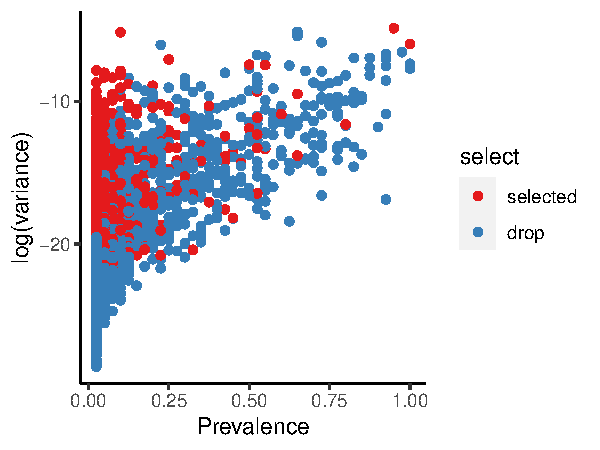
\includegraphics{workshop_files/figure-latex/unnamed-chunk-51-6.pdf}

\hypertarget{functional-prediction}{%
\section{Functional Prediction}\label{functional-prediction}}

\hypertarget{picrust2}{%
\subsection{PICRUSt2}\label{picrust2}}

Prepare files for running
\href{https://huttenhower.sph.harvard.edu/picrust/}{PICRUSt2} by
extracting the selected ASVs.

\begin{Shaded}
\begin{Highlighting}[]
\CommentTok{\# please ensure the "ASV.fasta" is in "output\_path" directory}
\NormalTok{output\_path }\OtherTok{\textless{}{-}} \StringTok{\textquotesingle{}\textasciitilde{}/Course/NDMC\_2025/tmp\textquotesingle{}}
\FunctionTok{dir}\NormalTok{(output\_path)}
\DocumentationTok{\#\# [1] "ASV\_table.txt"      "ASV\_taxa\_table.txt" "ASV.fasta"         }
\DocumentationTok{\#\# [4] "ASV.tree"           "for\_PICRUSt2.tsv"   "LEfSe\_tmp"         }
\DocumentationTok{\#\# [7] "PICRUSt2"           "PreLect\_tmp"        "ssuout"}
\NormalTok{selected\_id }\OtherTok{\textless{}{-}}\NormalTok{ featpropt}\SpecialCharTok{$}\NormalTok{FeatName[featpropt}\SpecialCharTok{$}\NormalTok{selected }\SpecialCharTok{==} \StringTok{\textquotesingle{}Selected\textquotesingle{}}\NormalTok{] }\CommentTok{\# selected by PreLect}
\NormalTok{data\_sub }\OtherTok{\textless{}{-}}\NormalTok{ data[selected\_id, ]  }\CommentTok{\# if you want to use whole ASVs, just data\_sub \textless{}{-} data}
\NormalTok{data\_sub }\OtherTok{\textless{}{-}} \FunctionTok{rbind}\NormalTok{(}\FunctionTok{colnames}\NormalTok{(data\_sub), data\_sub)}
\FunctionTok{colnames}\NormalTok{(data\_sub) }\OtherTok{\textless{}{-}} \ConstantTok{NULL}
\FunctionTok{rownames}\NormalTok{(data\_sub)[}\DecValTok{1}\NormalTok{] }\OtherTok{\textless{}{-}} \StringTok{"\#OTU ID"}
\FunctionTok{write.table}\NormalTok{(data\_sub, }\FunctionTok{paste0}\NormalTok{(output\_path,}\StringTok{"/for\_PICRUSt2.tsv"}\NormalTok{), }\AttributeTok{sep =} \StringTok{"}\SpecialCharTok{\textbackslash{}t}\StringTok{"}\NormalTok{, }\AttributeTok{quote=}\NormalTok{F, }\AttributeTok{col.names   =}\NormalTok{F)}
\end{Highlighting}
\end{Shaded}

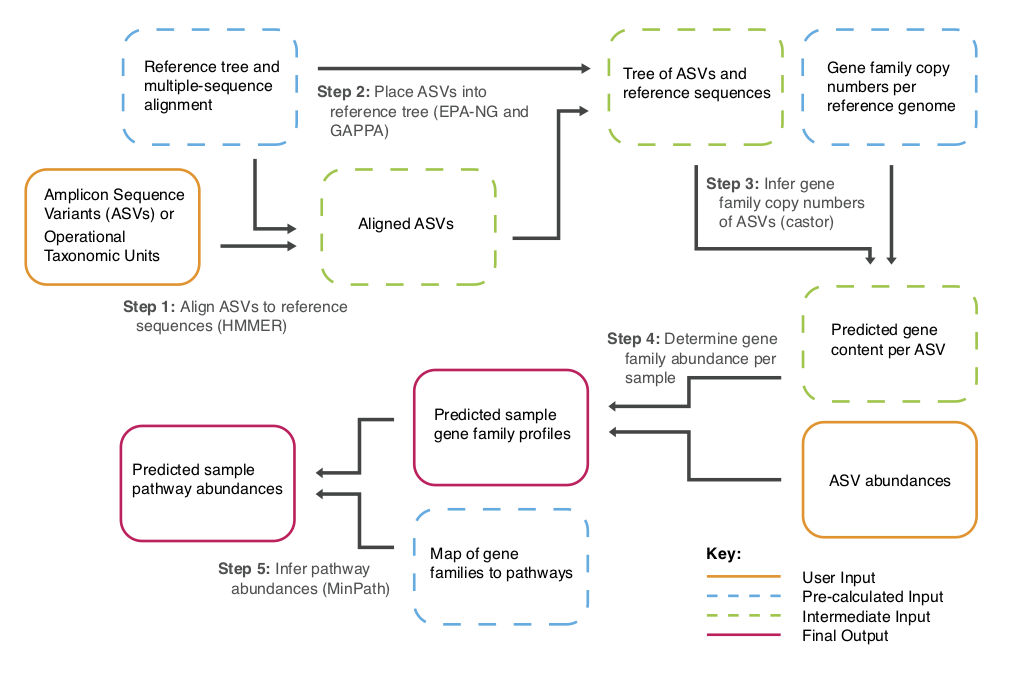
\includegraphics[width=0.8\textwidth,height=\textheight]{images/Fig14.png}

Conduct the PICRUSt2 pipeline via docker

\begin{Shaded}
\begin{Highlighting}[]
\CommentTok{\# Bash}
\CommentTok{\# run the PICRUSt2 pipeline}

\CommentTok{\# ensure the "ASV.fasta" and "for\_PICRUSt2.tsv" files are in the same directory }
\CommentTok{\# and set the working directory to that location before running this script.}
\ExtensionTok{$}\NormalTok{ cd \textasciitilde{}/Course/NDMC\_2025/tmp}
\ExtensionTok{$}\NormalTok{ docker run }\DataTypeTok{\textbackslash{}}
\NormalTok{$    }\AttributeTok{{-}u} \VariableTok{$UID}\NormalTok{:}\VariableTok{$(}\FunctionTok{id} \AttributeTok{{-}g}\VariableTok{)} \DataTypeTok{\textbackslash{} }             \CommentTok{\# perform this work as the current user.}
\ExtensionTok{$}    \AttributeTok{{-}i} \AttributeTok{{-}t} \DataTypeTok{\textbackslash{} }                       \CommentTok{\# interactive terminal mode, allowing you to interact with the container.}
\ExtensionTok{$}    \AttributeTok{{-}{-}rm} \DataTypeTok{\textbackslash{} }                        \CommentTok{\# automatically remove the container after it exits to save disk space.}
\ExtensionTok{$}    \AttributeTok{{-}v} \VariableTok{$(}\BuiltInTok{pwd}\VariableTok{)}\NormalTok{:/tmp }\DataTypeTok{\textbackslash{} }              \CommentTok{\# bind mount the current directory ($(pwd)) to /tmp in the container.}
\ExtensionTok{$}\NormalTok{    yincheng23/picrust2:0.2.0 }\DataTypeTok{\textbackslash{} }   \CommentTok{\# specify the Docker image to use; it will be pulled from Docker Hub if not available locally.}
\ExtensionTok{$}\NormalTok{    sh /bin/Run\_picrust2.sh 10     }\CommentTok{\# use the shell to execute the built{-}in script (Run\_picrust2.sh) with 10 cores for parallel processing.}
    
\CommentTok{\# the results will store as \textasciitilde{}/Course/NDMC\_2025/tmp/PICRUSt2}
\end{Highlighting}
\end{Shaded}

output file : ./PICRUSt2/KO/pred\_metagenome\_contrib.tsv - Represents
the relationship between functions and taxa.

output file : ./PICRUSt2/KO/pred\_metagenome\_unstrat\_descrip.tsv -
Contains KO (KEGG Orthology) abundances for each sample along with
detailed gene descriptions.

output file : ./PICRUSt2/KO/pred\_metagenome\_unstrat.tsv.gz - Provides
KO abundances for each sample.

Since \texttt{PICRUSt2} predicts gene abundance based on taxa abundance,
differential expression analysis using this approach may be less
convincing. Therefore, we adopted a \texttt{GSEA} strategy, ranking taxa
by fold change based on their abundance. Using insights provided by
\texttt{PICRUSt2}, we examined which species carry specific genes to
assess the KOs that are actively expressed or suppressed.

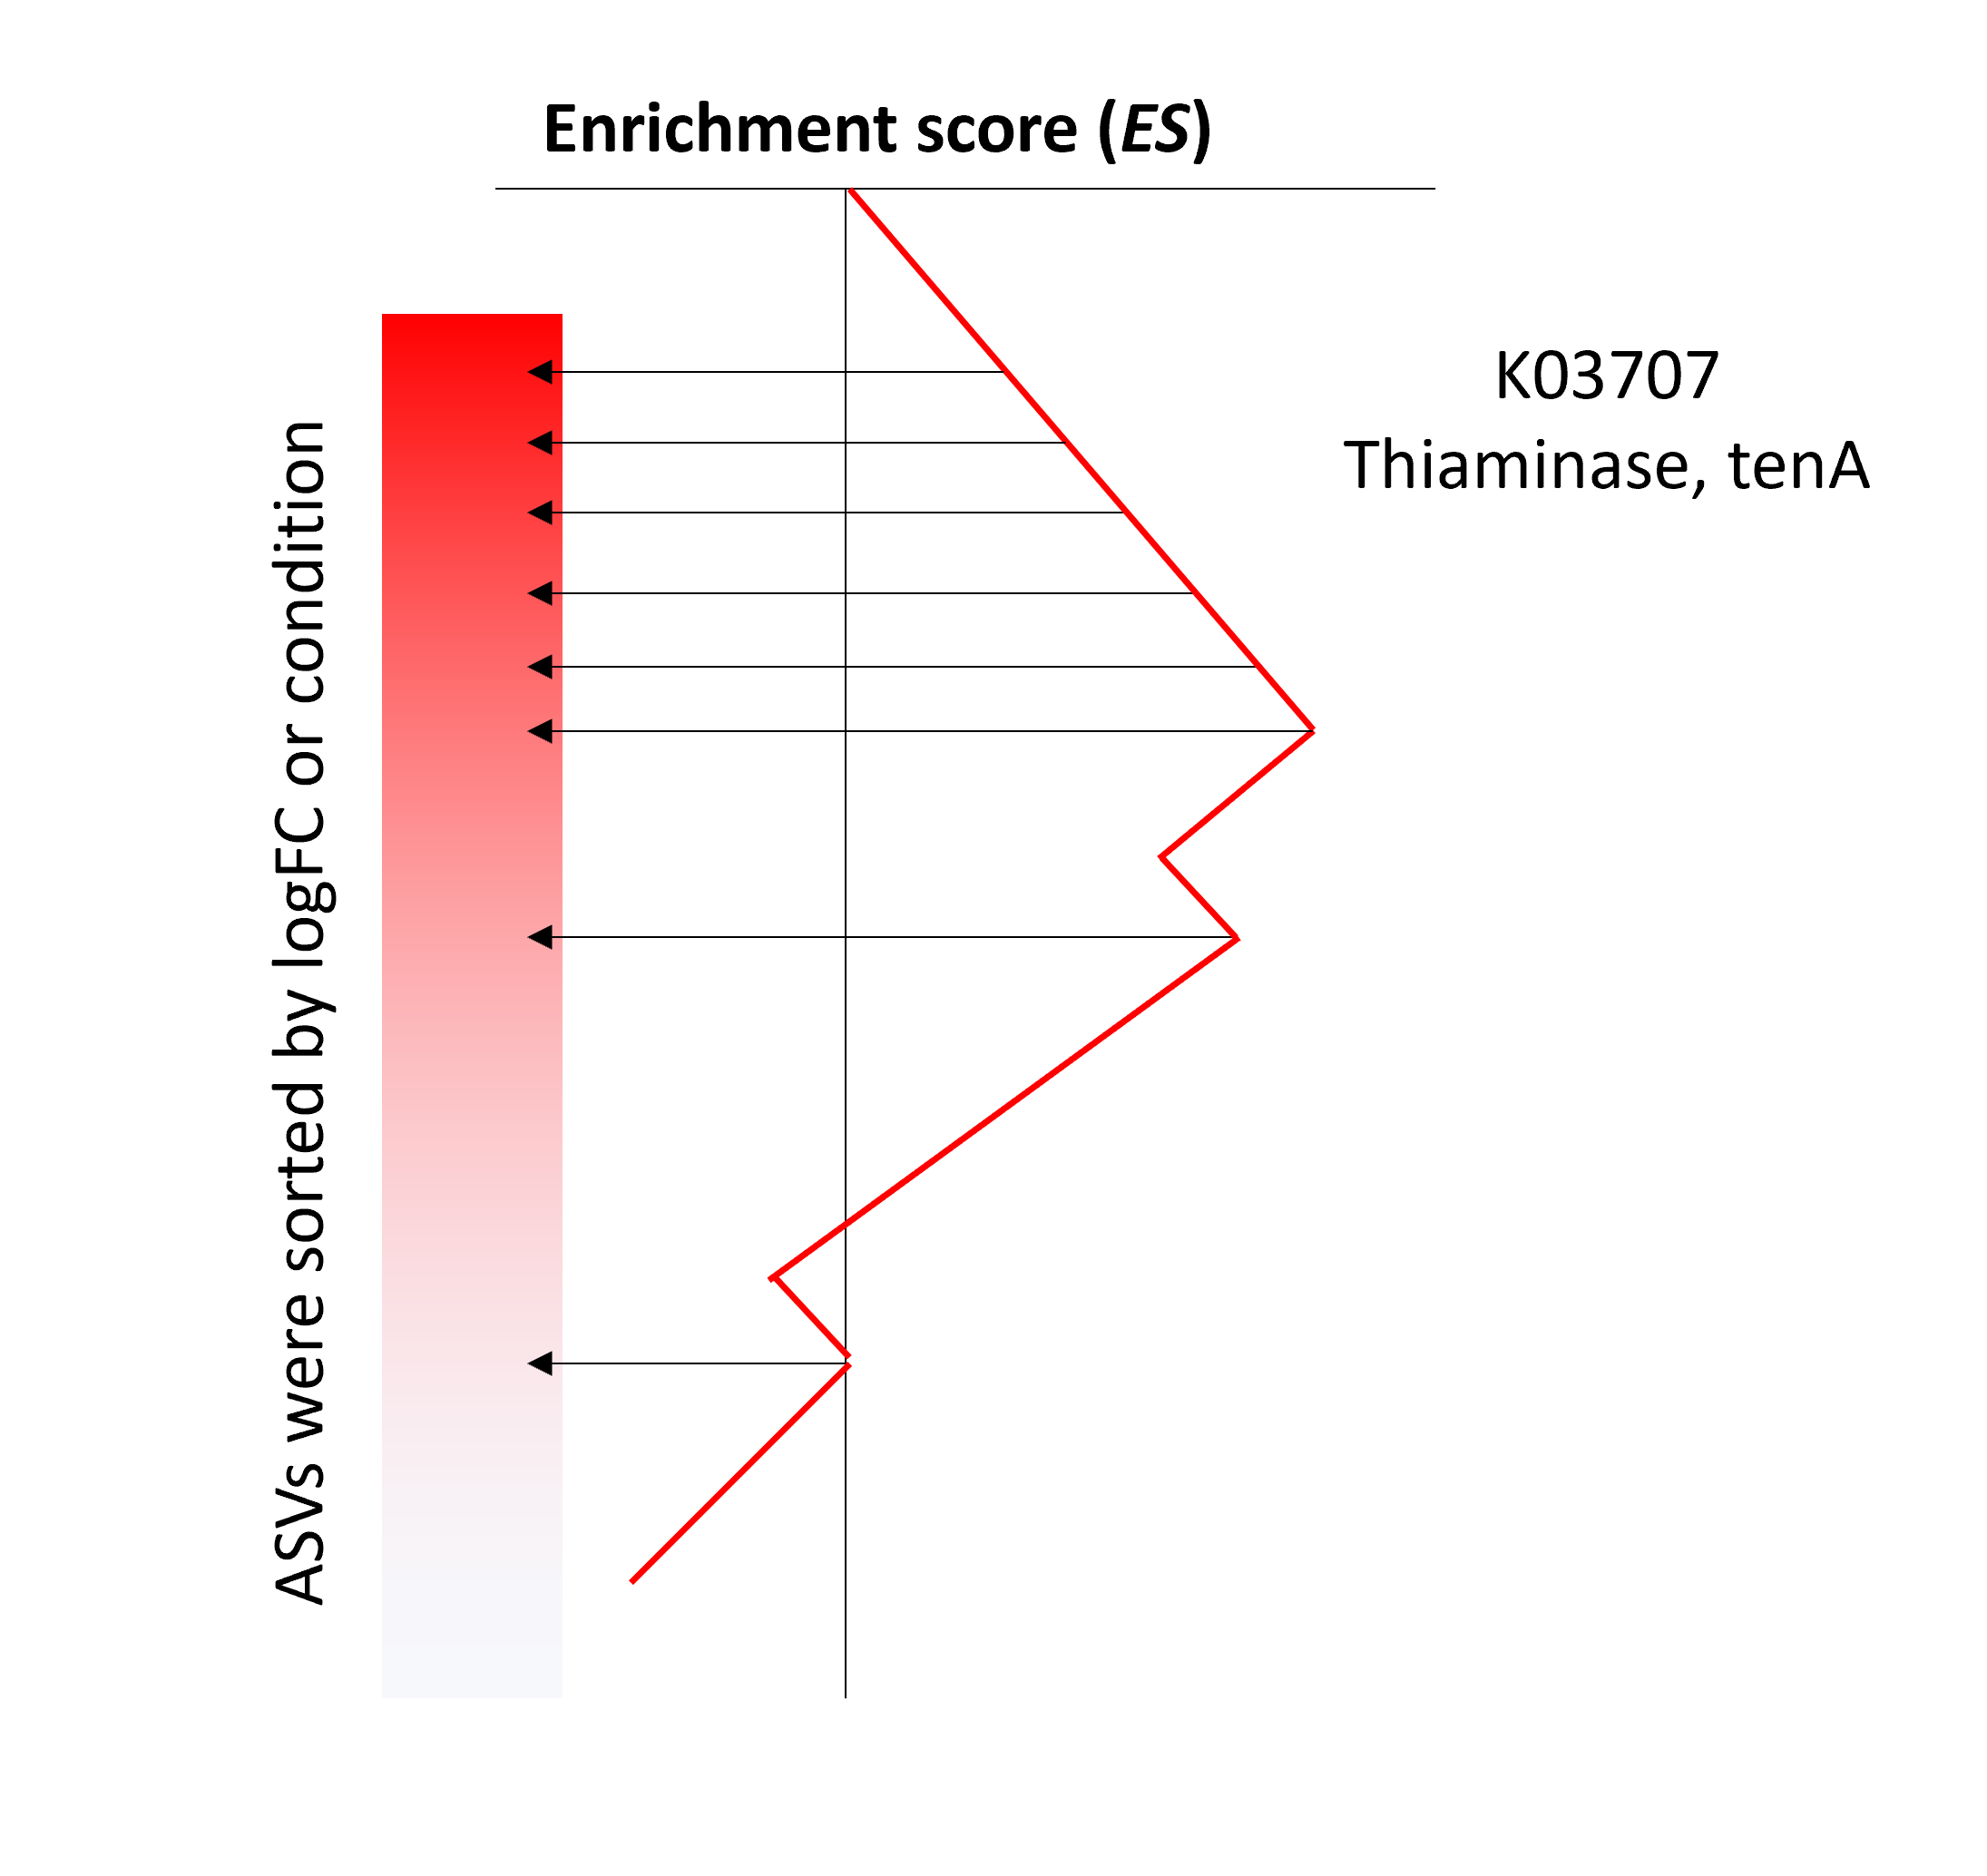
\includegraphics[width=0.7\textwidth,height=\textheight]{images/Fig15.png}

Conduct the GSEA with permutation test via \texttt{GSEATestwithFC} or
\texttt{GSEATest}

\begin{Shaded}
\begin{Highlighting}[]
\CommentTok{\# load the KO{-}taxa relationship file}
\CommentTok{\# output\_path is the directory you save the for\_PICRUSt2.tsv file}
\NormalTok{KOindex }\OtherTok{\textless{}{-}} \FunctionTok{read.table}\NormalTok{(}\FunctionTok{paste0}\NormalTok{(output\_path,}\StringTok{"/PICRUSt2/KO/pred\_metagenome\_contrib.tsv"}\NormalTok{), }\AttributeTok{sep =} \StringTok{"}\SpecialCharTok{\textbackslash{}t}\StringTok{"}\NormalTok{, }\AttributeTok{header =} \ConstantTok{TRUE}\NormalTok{)}

\CommentTok{\# extract the selected ASV identifiers}
\NormalTok{selected\_id }\OtherTok{\textless{}{-}}\NormalTok{ featpropt}\SpecialCharTok{$}\NormalTok{FeatName[featpropt}\SpecialCharTok{$}\NormalTok{selected }\SpecialCharTok{==} \StringTok{\textquotesingle{}Selected\textquotesingle{}}\NormalTok{]}

\CommentTok{\# Provide the raw count table for logFC calculation, subsetting with the selected ASVs.}
\CommentTok{\# Additionally, specify the labels for each sample and the name of the case sample group.}
\NormalTok{GSEAresult }\OtherTok{\textless{}{-}} \FunctionTok{GSEATestwithFC}\NormalTok{(KOindex, data[selected\_id, ], meta}\SpecialCharTok{$}\NormalTok{Class, }\StringTok{"Cancer"}\NormalTok{)}

\DocumentationTok{\#\# Building the KO{-}to{-}taxa mapper...}
\DocumentationTok{\#\# Done. In total, 5755 KOs need to be processed.}
\DocumentationTok{\#\# Shuffling the labels for GSEA...}
\DocumentationTok{\#\# Performing GSEA to identify activated KOs...}
\DocumentationTok{\#\#   |=======================================================================================================| 100\%}
\DocumentationTok{\#\# Shuffling the labels for GSEA...}
\DocumentationTok{\#\# Performing GSEA to identify suppressed KOs...}
\DocumentationTok{\#\#   |=======================================================================================================| 100\%}
\DocumentationTok{\#\# Done.}


\CommentTok{\# If the grouping variable is continuous (e.g., body mass index), use the following line instead:}
\CommentTok{\# GSEAresult \textless{}{-} GSEATest(KOindex, data[selected\_id, ], meta$body.mass.index)}
\end{Highlighting}
\end{Shaded}

Selected the enriched KOs with z-score

\begin{Shaded}
\begin{Highlighting}[]
\NormalTok{Actived\_result }\OtherTok{\textless{}{-}}\NormalTok{ GSEAresult}\SpecialCharTok{$}\NormalTok{Actived\_KO}
\NormalTok{Actived\_result }\OtherTok{\textless{}{-}}\NormalTok{ Actived\_result[}\SpecialCharTok{!}\FunctionTok{is.na}\NormalTok{(Actived\_result}\SpecialCharTok{$}\NormalTok{z), ]}
\NormalTok{Actived\_result }\OtherTok{\textless{}{-}}\NormalTok{ Actived\_result[Actived\_result}\SpecialCharTok{$}\NormalTok{z }\SpecialCharTok{\textgreater{}} \DecValTok{2}\NormalTok{,]}
\NormalTok{Actived\_result }\OtherTok{\textless{}{-}}\NormalTok{ Actived\_result[Actived\_result}\SpecialCharTok{$}\NormalTok{p }\SpecialCharTok{\textless{}} \FloatTok{0.05}\NormalTok{,]}
\FunctionTok{nrow}\NormalTok{(Actived\_result)}
\DocumentationTok{\#\# [1] 630}
\FunctionTok{head}\NormalTok{(Actived\_result)}
\DocumentationTok{\#\#        KO        ES        z     p}
\DocumentationTok{\#\# 1  K00121 0.3687500 2.066796 0.037}
\DocumentationTok{\#\# 20 K07304 0.2955083 3.399557 0.002}
\DocumentationTok{\#\# 35 K08296 0.4113924 2.298309 0.031}
\DocumentationTok{\#\# 42 K06145 0.5015198 2.027432 0.031}
\DocumentationTok{\#\# 43 K00567 0.2891499 3.072802 0.007}
\DocumentationTok{\#\# 62 K00365 0.8173653 2.101814 0.032}
\end{Highlighting}
\end{Shaded}

Since \texttt{PICRUSt2} does not provide detailed information for each
KO, we preprocess the KO-pathway table using the KEGG API.

\begin{Shaded}
\begin{Highlighting}[]
\NormalTok{kodb\_path }\OtherTok{\textless{}{-}} \FunctionTok{system.file}\NormalTok{(}\StringTok{"exdata"}\NormalTok{, }\StringTok{"total\_KO\_pathway.rds"}\NormalTok{, }\AttributeTok{package =} \StringTok{"PreLectR"}\NormalTok{)}
\NormalTok{KOinfo }\OtherTok{\textless{}{-}} \FunctionTok{readRDS}\NormalTok{(kodb\_path)}
\FunctionTok{head}\NormalTok{(KOinfo)}
\DocumentationTok{\#\#       KO        symbol                               name    mapid}
\DocumentationTok{\#\# 1 K00001 E1.1.1.1, adh alcohol dehydrogenase [EC:1.1.1.1] map00010}
\DocumentationTok{\#\# 2 K00001 E1.1.1.1, adh alcohol dehydrogenase [EC:1.1.1.1] map00071}
\DocumentationTok{\#\# 3 K00001 E1.1.1.1, adh alcohol dehydrogenase [EC:1.1.1.1] map00350}
\DocumentationTok{\#\# 4 K00001 E1.1.1.1, adh alcohol dehydrogenase [EC:1.1.1.1] map00620}
\DocumentationTok{\#\# 5 K00001 E1.1.1.1, adh alcohol dehydrogenase [EC:1.1.1.1] map00625}
\DocumentationTok{\#\# 6 K00001 E1.1.1.1, adh alcohol dehydrogenase [EC:1.1.1.1] map00626}
\DocumentationTok{\#\#                                     pathway}
\DocumentationTok{\#\# 1              Glycolysis / Gluconeogenesis}
\DocumentationTok{\#\# 2                    Fatty acid degradation}
\DocumentationTok{\#\# 3                       Tyrosine metabolism}
\DocumentationTok{\#\# 4                       Pyruvate metabolism}
\DocumentationTok{\#\# 5 Chloroalkane and chloroalkene degradation}
\DocumentationTok{\#\# 6                   Naphthalene degradation}
\end{Highlighting}
\end{Shaded}

Examining the condition enriched pathway with Fisher's exact test via
\texttt{PathwayEnrichment}

\begin{Shaded}
\begin{Highlighting}[]
\NormalTok{KOinfo }\OtherTok{\textless{}{-}}\NormalTok{ KOinfo[KOinfo}\SpecialCharTok{$}\NormalTok{KO }\SpecialCharTok{\%in\%} \FunctionTok{unique}\NormalTok{(KOindex}\SpecialCharTok{$}\NormalTok{function.), ]}
\NormalTok{Actived\_result }\OtherTok{\textless{}{-}}\NormalTok{ GSEAresult}\SpecialCharTok{$}\NormalTok{Actived\_KO}
\NormalTok{Actived\_result }\OtherTok{\textless{}{-}}\NormalTok{ Actived\_result[}\SpecialCharTok{!}\FunctionTok{is.na}\NormalTok{(Actived\_result}\SpecialCharTok{$}\NormalTok{z), ]}
\NormalTok{Actived\_result }\OtherTok{\textless{}{-}}\NormalTok{ Actived\_result[Actived\_result}\SpecialCharTok{$}\NormalTok{z }\SpecialCharTok{\textgreater{}} \DecValTok{2}\NormalTok{,]}
\NormalTok{Actived\_result }\OtherTok{\textless{}{-}}\NormalTok{ Actived\_result[Actived\_result}\SpecialCharTok{$}\NormalTok{p }\SpecialCharTok{\textless{}} \FloatTok{0.05}\NormalTok{,]}
\NormalTok{selected\_KOs }\OtherTok{\textless{}{-}}\NormalTok{ Actived\_result}\SpecialCharTok{$}\NormalTok{KO}

\NormalTok{enrichPW }\OtherTok{\textless{}{-}} \FunctionTok{PathwayEnrichment}\NormalTok{(selected\_KOs, KOinfo)}
\NormalTok{enrichPW}\SpecialCharTok{$}\NormalTok{q }\OtherTok{\textless{}{-}} \FunctionTok{p.adjust}\NormalTok{(enrichPW}\SpecialCharTok{$}\NormalTok{p, }\AttributeTok{method =} \StringTok{\textquotesingle{}fdr\textquotesingle{}}\NormalTok{)}
\NormalTok{enrichPW }\OtherTok{\textless{}{-}}\NormalTok{ enrichPW[enrichPW}\SpecialCharTok{$}\NormalTok{q }\SpecialCharTok{\textless{}} \FloatTok{0.05}\NormalTok{, ]}
\FunctionTok{nrow}\NormalTok{(enrichPW)}
\DocumentationTok{\#\# [1] 6}

\FunctionTok{head}\NormalTok{(enrichPW)}
\DocumentationTok{\#\#                                 pathway       id count     ratio            p}
\DocumentationTok{\#\# 26    Degradation of aromatic compounds map01220    18 0.3829787 9.848597e{-}07}
\DocumentationTok{\#\# 31               Lipoic acid metabolism map00785     9 0.4090909 2.743792e{-}04}
\DocumentationTok{\#\# 34            Oxidative phosphorylation map00190    23 0.3026316 4.214420e{-}06}
\DocumentationTok{\#\# 64                 Benzoate degradation map00362    18 0.4000000 4.614879e{-}07}
\DocumentationTok{\#\# 112          Fluorobenzoate degradation map00364     6 0.6666667 1.007485e{-}04}
\DocumentationTok{\#\# 133 Biofilm formation {-} Vibrio cholerae map05111    14 0.4000000 7.841760e{-}06}
\DocumentationTok{\#\#     odds\_ratio            q}
\DocumentationTok{\#\# 26    5.161160 9.159195e{-}05}
\DocumentationTok{\#\# 31    5.756061 8.505756e{-}03}
\DocumentationTok{\#\# 34    3.605573 2.612941e{-}04}
\DocumentationTok{\#\# 64    5.543134 8.583675e{-}05}
\DocumentationTok{\#\# 112  16.614397 3.747845e{-}03}
\DocumentationTok{\#\# 133   5.572086 3.646418e{-}04}
\end{Highlighting}
\end{Shaded}

\begin{Shaded}
\begin{Highlighting}[]
\NormalTok{enrichPW}\SpecialCharTok{$}\NormalTok{pathway }\OtherTok{\textless{}{-}} \FunctionTok{factor}\NormalTok{(enrichPW}\SpecialCharTok{$}\NormalTok{pathway, }\AttributeTok{levels =}\NormalTok{ enrichPW}\SpecialCharTok{$}\NormalTok{pathway[}\FunctionTok{order}\NormalTok{(enrichPW}\SpecialCharTok{$}\NormalTok{count)])}
\FunctionTok{ggplot}\NormalTok{(enrichPW, }\FunctionTok{aes}\NormalTok{(}\AttributeTok{x =}\NormalTok{ pathway, }\AttributeTok{y =}\NormalTok{ count, }\AttributeTok{fill =}\NormalTok{ q)) }\SpecialCharTok{+} \FunctionTok{ggtitle}\NormalTok{(}\StringTok{\textquotesingle{}Enhanced in colorectal cancer\textquotesingle{}}\NormalTok{) }\SpecialCharTok{+}
  \FunctionTok{geom\_bar}\NormalTok{(}\AttributeTok{stat=}\StringTok{"identity"}\NormalTok{,}\AttributeTok{colour =} \StringTok{"black"}\NormalTok{,}\AttributeTok{size =} \FloatTok{0.1}\NormalTok{) }\SpecialCharTok{+}  \FunctionTok{coord\_flip}\NormalTok{() }\SpecialCharTok{+} \FunctionTok{labs}\NormalTok{(}\AttributeTok{y =} \StringTok{\textquotesingle{}KO Hits\textquotesingle{}}\NormalTok{, }\AttributeTok{fill =} \StringTok{"q{-}value"}\NormalTok{) }\SpecialCharTok{+}
  \FunctionTok{scale\_fill\_continuous}\NormalTok{(}\AttributeTok{low =} \StringTok{"red"}\NormalTok{, }\AttributeTok{high =} \StringTok{"blue"}\NormalTok{, }\AttributeTok{limits =} \FunctionTok{range}\NormalTok{(enrichPW}\SpecialCharTok{$}\NormalTok{q)) }\SpecialCharTok{+}
  \FunctionTok{theme}\NormalTok{(}\AttributeTok{axis.text.y =} \FunctionTok{element\_text}\NormalTok{(}\AttributeTok{color=}\StringTok{\textquotesingle{}black\textquotesingle{}}\NormalTok{, }\AttributeTok{size=}\StringTok{\textquotesingle{}10\textquotesingle{}}\NormalTok{),}
        \AttributeTok{axis.line =} \FunctionTok{element\_line}\NormalTok{(}\AttributeTok{linetype =} \DecValTok{1}\NormalTok{,}\AttributeTok{colour =} \StringTok{\textquotesingle{}black\textquotesingle{}}\NormalTok{),}
        \AttributeTok{axis.title.y =} \FunctionTok{element\_blank}\NormalTok{(),}
        \AttributeTok{panel.background =} \FunctionTok{element\_rect}\NormalTok{(}\FunctionTok{I}\NormalTok{(}\DecValTok{0}\NormalTok{)),}
        \AttributeTok{panel.grid.major =} \FunctionTok{element\_line}\NormalTok{(}\AttributeTok{colour =} \ConstantTok{NA}\NormalTok{),}
        \AttributeTok{panel.grid.minor =} \FunctionTok{element\_line}\NormalTok{(}\AttributeTok{colour =} \ConstantTok{NA}\NormalTok{)) }\SpecialCharTok{+} \FunctionTok{coord\_flip}\NormalTok{()}
\end{Highlighting}
\end{Shaded}

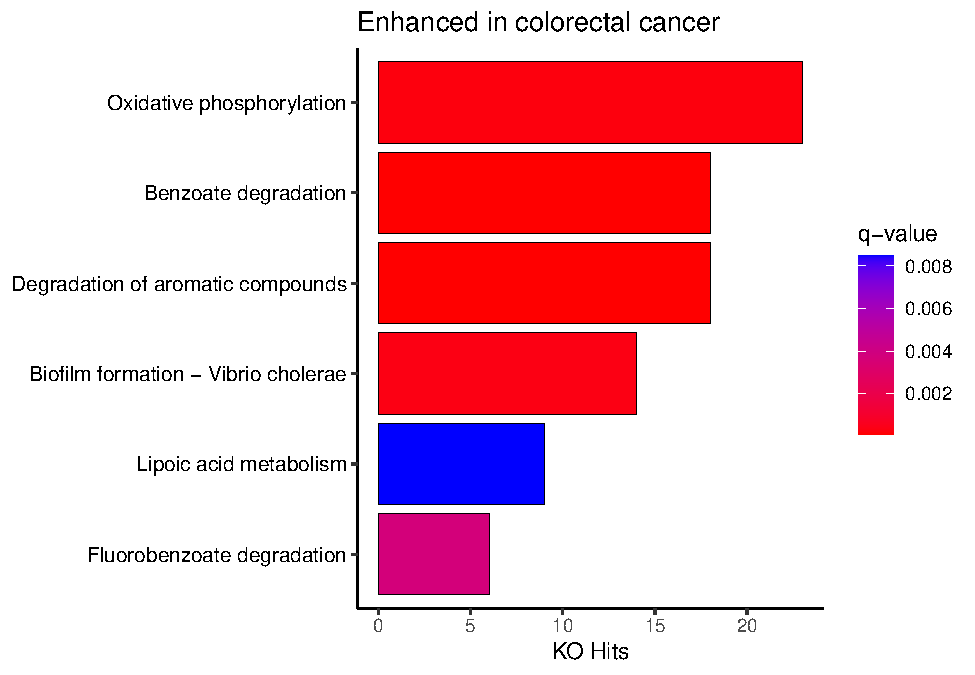
\includegraphics{workshop_files/figure-latex/unnamed-chunk-58-1.pdf}

\hypertarget{rpm}{%
\subsection{RPM}\label{rpm}}

Reference Pathways Mapper (RPM) utilizes a reference pathways database,
which is a flat file listing pathway/module reactions in sequential
order. Tab-separated reactions indicate alternative reactions (OR
operation), while line breaks and comma-separated reactions represent
reactions that are all required for pathway completion (AND operation).

Below is a snippet from the
\texttt{human\ gut\ metabolic\ modules\ (GMMs)} database, as described
by \href{https://www.nature.com/articles/nmicrobiol201688}{Vieira-Silva
et al.~2016}.

\begin{Shaded}
\begin{Highlighting}[]
\NormalTok{MF0001  arabinoxylan degradation}
\NormalTok{K01209  K15921  K01181  K01198  K15531  K18205}
\SpecialCharTok{/}\ErrorTok{//}
\NormalTok{MF0003  pectin degradation I}
\NormalTok{K01051}
\NormalTok{K01184,K01213   K18650}
\SpecialCharTok{/}\ErrorTok{//}
\NormalTok{MF0103  mucin degradation}
\NormalTok{K01186}
\NormalTok{K05970}
\NormalTok{K01132  K01135  K01137  K01205}
\NormalTok{K01207  K12373  K14459}
\NormalTok{K01205  K01207  K12373  K01227  K13714}
\NormalTok{K01206}
\SpecialCharTok{/}\ErrorTok{//}
\end{Highlighting}
\end{Shaded}

\hypertarget{installation}{%
\paragraph{Installation}\label{installation}}

According to
\href{https://github.com/omixer/omixer-rpmR?tab=readme-ov-file}{original
repository}

\begin{Shaded}
\begin{Highlighting}[]
\ExtensionTok{$}\NormalTok{ wget https://github.com/omixer/omixer{-}rpmR/releases/download/0.3.3/omixerRpm\_0.3.3.tar.gz}
\ExtensionTok{$}\NormalTok{ R CMD INSTALL omixerRpm\_0.3.3.tar.gz}
\end{Highlighting}
\end{Shaded}

\hypertarget{pathway-mapping}{%
\paragraph{Pathway mapping}\label{pathway-mapping}}

\begin{Shaded}
\begin{Highlighting}[]
\FunctionTok{library}\NormalTok{(omixerRpm)}
\FunctionTok{library}\NormalTok{(dplyr)}
\FunctionTok{library}\NormalTok{(tidyr)}

\NormalTok{KOtable }\OtherTok{\textless{}{-}} \FunctionTok{read.table}\NormalTok{(}\FunctionTok{paste0}\NormalTok{(output\_path,}\StringTok{"/PICRUSt2/KO/pred\_metagenome\_contrib.tsv"}\NormalTok{), }\AttributeTok{sep =} \StringTok{"}\SpecialCharTok{\textbackslash{}t}\StringTok{"}\NormalTok{, }\AttributeTok{header =} \ConstantTok{TRUE}\NormalTok{)}

\FunctionTok{colnames}\NormalTok{(KOtable)[}\DecValTok{2}\NormalTok{] }\OtherTok{\textless{}{-}} \StringTok{\textquotesingle{}fun\textquotesingle{}}
\NormalTok{sumtb }\OtherTok{\textless{}{-}}\NormalTok{ KOtable }\SpecialCharTok{\%\textgreater{}\%} \FunctionTok{group\_by}\NormalTok{(sample, fun) }\SpecialCharTok{\%\textgreater{}\%} \FunctionTok{summarise}\NormalTok{(}\AttributeTok{sum\_rel\_function\_abun=}\FunctionTok{sum}\NormalTok{(taxon\_rel\_function\_abun))}
\NormalTok{tmp }\OtherTok{\textless{}{-}} \FunctionTok{spread}\NormalTok{(sumtb, }\AttributeTok{key =}\NormalTok{ sample, }\AttributeTok{value =}\NormalTok{ sum\_rel\_function\_abun)}
\FunctionTok{colnames}\NormalTok{(tmp)[}\DecValTok{1}\NormalTok{] }\OtherTok{\textless{}{-}} \StringTok{\textquotesingle{}entry\textquotesingle{}}
\NormalTok{tmp[}\FunctionTok{is.na}\NormalTok{(tmp)] }\OtherTok{\textless{}{-}} \DecValTok{0}

\NormalTok{mods }\OtherTok{\textless{}{-}} \FunctionTok{rpm}\NormalTok{(tmp, }\AttributeTok{minimum.coverage=}\FloatTok{0.3}\NormalTok{, }\AttributeTok{annotation =} \DecValTok{1}\NormalTok{)}
\DocumentationTok{\#\# [1] "Loaded GMMs.v1.07"}
\NormalTok{db }\OtherTok{\textless{}{-}} \FunctionTok{loadDefaultDB}\NormalTok{()}
\DocumentationTok{\#\# [1] "Loaded GMMs.v1.07"}
\FunctionTok{getNames}\NormalTok{(db, mods}\SpecialCharTok{@}\NormalTok{annotation[}\DecValTok{1}\NormalTok{,])}
\DocumentationTok{\#\# [1] "ribose degradation"}
\NormalTok{coverage }\OtherTok{\textless{}{-}} \FunctionTok{asDataFrame}\NormalTok{(mods, }\StringTok{"coverage"}\NormalTok{)}
\NormalTok{module  }\OtherTok{\textless{}{-}}\NormalTok{ mods}\SpecialCharTok{@}\NormalTok{abundance}
\FunctionTok{rownames}\NormalTok{(module) }\OtherTok{\textless{}{-}}\NormalTok{ coverage}\SpecialCharTok{$}\NormalTok{Description}
\FunctionTok{head}\NormalTok{(module)}
\DocumentationTok{\#\#                                ERR475527 ERR475549    ERR475504   ERR475529}
\DocumentationTok{\#\# ribose degradation           35.16937498  35.17516 3.098085e+01  55.4419850}
\DocumentationTok{\#\# tyrosine degradation II       0.00736405   0.00000 0.000000e+00   0.1532172}
\DocumentationTok{\#\# aspartate degradation I      56.20638043  68.65780 5.569382e+01  54.3297498}
\DocumentationTok{\#\# tryptophan degradation        5.20525631   1.12031 1.160618e+01   3.2142130}
\DocumentationTok{\#\# tyrosine degradation I       50.58997819 101.04308 5.424949e+01 104.9491610}
\DocumentationTok{\#\# galacturonate degradation II  0.00000000   0.00000 9.507594e{-}04   0.0000000}
\DocumentationTok{\#\#                               ERR475528   ERR475545   ERR475500   ERR475588}
\DocumentationTok{\#\# ribose degradation           27.8606223 27.09122669 63.79307368 50.59532850}
\DocumentationTok{\#\# tyrosine degradation II       0.0159962  0.00000000  0.14151356  0.00000000}
\DocumentationTok{\#\# aspartate degradation I      79.0703436 87.57625174 87.98962719 63.41611505}
\DocumentationTok{\#\# tryptophan degradation       10.6104558 21.77601754  2.87128420 33.18194936}
\DocumentationTok{\#\# tyrosine degradation I       51.9888339 60.34117553 53.45470956 41.96002481}
\DocumentationTok{\#\# galacturonate degradation II  0.0000000  0.01126817  0.01038632  0.03272184}
\DocumentationTok{\#\#                              ERR475547  ERR475541 ERR475485    ERR475540}
\DocumentationTok{\#\# ribose degradation            31.55949 28.4148131 25.326445  23.52926496}
\DocumentationTok{\#\# tyrosine degradation II        0.00000  0.1387234  0.000000   0.08120360}
\DocumentationTok{\#\# aspartate degradation I       87.24203 59.8965261 49.600167 117.38540049}
\DocumentationTok{\#\# tryptophan degradation        15.62138  4.5938590  3.226059  16.50346978}
\DocumentationTok{\#\# tyrosine degradation I        52.56882 51.8888387 50.360550  58.77502133}
\DocumentationTok{\#\# galacturonate degradation II   0.00000  0.0175545  0.000000   0.02160463}
\DocumentationTok{\#\#                              ERR475562    ERR475584   ERR475521    ERR475565}
\DocumentationTok{\#\# ribose degradation            21.27139 22.234725150 21.73869043 18.653580678}
\DocumentationTok{\#\# tyrosine degradation II        0.00000  0.019633212  0.08697272  0.095860634}
\DocumentationTok{\#\# aspartate degradation I       61.78199 51.502887344 71.82182553 36.918989696}
\DocumentationTok{\#\# tryptophan degradation        21.02328  4.870319828 13.28846530 12.576196223}
\DocumentationTok{\#\# tyrosine degradation I        56.55310 51.969782663 55.30241396 52.756376669}
\DocumentationTok{\#\# galacturonate degradation II   0.00000  0.005960082  0.04027999  0.002396516}
\DocumentationTok{\#\#                                ERR475586  ERR475580    ERR475484 ERR475561}
\DocumentationTok{\#\# ribose degradation           46.99615938 34.6893540  27.80085184 36.651911}
\DocumentationTok{\#\# tyrosine degradation II       0.43654951  0.0000000   0.03075402  0.000000}
\DocumentationTok{\#\# aspartate degradation I      78.71544166 48.5301653  63.21129882 53.275009}
\DocumentationTok{\#\# tryptophan degradation       14.27417268  8.0092019   6.06292426  1.126657}
\DocumentationTok{\#\# tyrosine degradation I       50.86031496 50.9725785 101.77878685 50.407778}
\DocumentationTok{\#\# galacturonate degradation II  0.01942096  0.0221183   0.00000000  0.000000}
\DocumentationTok{\#\#                                ERR475483 ERR475560  ERR475590   ERR475518}
\DocumentationTok{\#\# ribose degradation            29.1709203 45.736165 29.9555807 28.04525333}
\DocumentationTok{\#\# tyrosine degradation II        0.0000000  0.000000  0.0000000  0.01163850}
\DocumentationTok{\#\# aspartate degradation I       58.3060655 41.854488 72.7521866 49.14149961}
\DocumentationTok{\#\# tryptophan degradation         0.6992597  2.599723 19.2800891  3.64808639}
\DocumentationTok{\#\# tyrosine degradation I       102.9874650 49.899148 54.3941577 53.93726862}
\DocumentationTok{\#\# galacturonate degradation II   0.0000000  0.000000  0.1025416  0.02168992}
\DocumentationTok{\#\#                                ERR475534    ERR475478    ERR475555    ERR475577}
\DocumentationTok{\#\# ribose degradation           31.02395184 3.450413e+01 3.441916e+01 48.548405549}
\DocumentationTok{\#\# tyrosine degradation II       0.05004837 1.083518e{-}01 0.000000e+00  0.127484993}
\DocumentationTok{\#\# aspartate degradation I      55.09630176 5.241802e+01 6.256350e+01 57.795267824}
\DocumentationTok{\#\# tryptophan degradation        2.10620205 6.076617e+00 3.097498e{-}01  1.738492718}
\DocumentationTok{\#\# tyrosine degradation I       49.95218205 1.067859e+02 1.007209e+02 51.958954529}
\DocumentationTok{\#\# galacturonate degradation II  0.00000000 8.334751e{-}03 3.997287e{-}03  0.009393631}
\DocumentationTok{\#\#                                ERR475513   ERR475579   ERR475554    ERR475576}
\DocumentationTok{\#\# ribose degradation           31.59691328 22.92837864 18.73800856  37.82823763}
\DocumentationTok{\#\# tyrosine degradation II       0.02523416  0.15720108  0.06997963   0.31456905}
\DocumentationTok{\#\# aspartate degradation I      90.11875161 91.17260136 76.39798496 148.87959127}
\DocumentationTok{\#\# tryptophan degradation       25.45861537 23.86014480  1.94103675  59.91196697}
\DocumentationTok{\#\# tyrosine degradation I       57.19484500 45.59180272 50.44075281  74.74717910}
\DocumentationTok{\#\# galacturonate degradation II  0.07131394  0.02515217  0.00000000   0.01037918}
\DocumentationTok{\#\#                                 ERR475476  ERR475553    ERR475493    ERR475591}
\DocumentationTok{\#\# ribose degradation           23.014066166 40.9080176 2.808007e+01 27.068650441}
\DocumentationTok{\#\# tyrosine degradation II       0.044911132  0.0000000 1.930299e+00  0.002083388}
\DocumentationTok{\#\# aspartate degradation I      67.459882221 85.0328572 4.551332e+01 62.929806811}
\DocumentationTok{\#\# tryptophan degradation       12.719718609  0.5422964 5.907959e+00  8.902784854}
\DocumentationTok{\#\# tyrosine degradation I       53.791136776 99.3264616 1.021285e+02 56.030165476}
\DocumentationTok{\#\# galacturonate degradation II  0.009710515  0.0000000 7.034617e{-}03  0.048438766}
\DocumentationTok{\#\#                               ERR475473   ERR475550  ERR475594    ERR475480}
\DocumentationTok{\#\# ribose degradation           19.1812121 32.08871268 62.5142559  31.15863997}
\DocumentationTok{\#\# tyrosine degradation II       0.1721522  0.03903622  0.3954753   0.00000000}
\DocumentationTok{\#\# aspartate degradation I      58.6562929 78.48988082 94.8305828  35.21222110}
\DocumentationTok{\#\# tryptophan degradation        4.5486796  0.62264043  5.3451859   0.16811702}
\DocumentationTok{\#\# tyrosine degradation I       58.1781156 49.20786881 61.6465806 106.09704137}
\DocumentationTok{\#\# galacturonate degradation II  0.0000000  0.00000000  0.2272061   0.03641655}
\end{Highlighting}
\end{Shaded}

\hypertarget{module-visualization}{%
\paragraph{Module visualization}\label{module-visualization}}

Please ensure that the dataframe \texttt{meta} has a column named
\texttt{group}, which records the grouping information.

Only binary grouping is supported in the following process.

\begin{Shaded}
\begin{Highlighting}[]
\NormalTok{meta}\SpecialCharTok{$}\NormalTok{group }\OtherTok{\textless{}{-}}\NormalTok{ meta}\SpecialCharTok{$}\NormalTok{Class }\CommentTok{\# pleas ensure this}

\CommentTok{\# GMMviz function is sourced from utils.R}
\NormalTok{results }\OtherTok{\textless{}{-}} \FunctionTok{GMMviz}\NormalTok{(module, meta, }\StringTok{\textquotesingle{}Normal\textquotesingle{}}\NormalTok{) }\CommentTok{\# please assign the control name as the third parameter.}
\NormalTok{sigdf }\OtherTok{\textless{}{-}}\NormalTok{ results}\SpecialCharTok{$}\NormalTok{significance\_df}
\NormalTok{boxdf }\OtherTok{\textless{}{-}}\NormalTok{ results}\SpecialCharTok{$}\NormalTok{relative\_abundance\_df}
\NormalTok{covdf }\OtherTok{\textless{}{-}}\NormalTok{ results}\SpecialCharTok{$}\NormalTok{coverage\_df}

\NormalTok{sigdf }\OtherTok{\textless{}{-}}\NormalTok{ sigdf[sigdf}\SpecialCharTok{$}\NormalTok{p }\SpecialCharTok{\textless{}} \FloatTok{0.01}\NormalTok{, ]}
\NormalTok{boxdf }\OtherTok{\textless{}{-}}\NormalTok{ boxdf[boxdf}\SpecialCharTok{$}\NormalTok{module }\SpecialCharTok{\%in\%}\NormalTok{ sigdf}\SpecialCharTok{$}\NormalTok{module,]}
\NormalTok{covdf }\OtherTok{\textless{}{-}}\NormalTok{ covdf[covdf}\SpecialCharTok{$}\NormalTok{module }\SpecialCharTok{\%in\%}\NormalTok{ sigdf}\SpecialCharTok{$}\NormalTok{module,]}

\NormalTok{module\_order }\OtherTok{\textless{}{-}}\NormalTok{ sigdf}\SpecialCharTok{$}\NormalTok{module[}\FunctionTok{order}\NormalTok{(sigdf}\SpecialCharTok{$}\NormalTok{log2FC, }\AttributeTok{decreasing =}\NormalTok{ F)]}
\NormalTok{sigdf}\SpecialCharTok{$}\NormalTok{module }\OtherTok{\textless{}{-}} \FunctionTok{factor}\NormalTok{(sigdf}\SpecialCharTok{$}\NormalTok{module, }\AttributeTok{levels =}\NormalTok{ module\_order)}
\NormalTok{boxdf}\SpecialCharTok{$}\NormalTok{module }\OtherTok{\textless{}{-}} \FunctionTok{factor}\NormalTok{(boxdf}\SpecialCharTok{$}\NormalTok{module, }\AttributeTok{levels =}\NormalTok{ module\_order)}
\NormalTok{covdf}\SpecialCharTok{$}\NormalTok{module }\OtherTok{\textless{}{-}} \FunctionTok{factor}\NormalTok{(covdf}\SpecialCharTok{$}\NormalTok{module, }\AttributeTok{levels =}\NormalTok{ module\_order)}

\NormalTok{mycolor }\OtherTok{\textless{}{-}} \FunctionTok{c}\NormalTok{(}\StringTok{"Normal"} \OtherTok{=} \StringTok{"\#FFCC22"}\NormalTok{, }\StringTok{"Cancer"} \OtherTok{=} \StringTok{"\#EE7700"}\NormalTok{) }\CommentTok{\# color assignment}
\NormalTok{p1 }\OtherTok{\textless{}{-}} \FunctionTok{ggplot}\NormalTok{(boxdf, }\FunctionTok{aes}\NormalTok{(}\AttributeTok{x =}\NormalTok{ module, }\AttributeTok{y =}\NormalTok{ value, }\AttributeTok{color =}\NormalTok{ group)) }\SpecialCharTok{+}  \FunctionTok{coord\_flip}\NormalTok{() }\SpecialCharTok{+}
      \FunctionTok{scale\_x\_discrete}\NormalTok{() }\SpecialCharTok{+}
      \FunctionTok{ylab}\NormalTok{(}\StringTok{"Relative abundance (\%)"}\NormalTok{) }\SpecialCharTok{+} \FunctionTok{scale\_color\_manual}\NormalTok{(}\AttributeTok{values =}\NormalTok{ mycolor) }\SpecialCharTok{+}
      \FunctionTok{theme}\NormalTok{(}\AttributeTok{panel.background =} \FunctionTok{element\_rect}\NormalTok{(}\AttributeTok{fill =} \StringTok{\textquotesingle{}transparent\textquotesingle{}}\NormalTok{),}
        \AttributeTok{panel.grid =} \FunctionTok{element\_blank}\NormalTok{(),}
        \AttributeTok{axis.ticks.length =} \FunctionTok{unit}\NormalTok{(}\FloatTok{0.4}\NormalTok{,}\StringTok{"lines"}\NormalTok{),}
        \AttributeTok{axis.ticks =} \FunctionTok{element\_line}\NormalTok{(}\AttributeTok{color=}\StringTok{\textquotesingle{}black\textquotesingle{}}\NormalTok{),}
        \AttributeTok{axis.line =} \FunctionTok{element\_line}\NormalTok{(}\AttributeTok{colour =} \StringTok{"black"}\NormalTok{),}
        \AttributeTok{axis.text.y =} \FunctionTok{element\_text}\NormalTok{(}\AttributeTok{colour=}\StringTok{\textquotesingle{}black\textquotesingle{}}\NormalTok{,}\AttributeTok{size=}\DecValTok{12}\NormalTok{),}
        \AttributeTok{axis.title.y =} \FunctionTok{element\_blank}\NormalTok{(),}
        \AttributeTok{legend.title=}\FunctionTok{element\_blank}\NormalTok{(),}
        \AttributeTok{legend.position =} \StringTok{\textquotesingle{}top\textquotesingle{}}\NormalTok{)}
\NormalTok{sing }\OtherTok{=} \DecValTok{1}
\ControlFlowTok{for}\NormalTok{ (i }\ControlFlowTok{in} \DecValTok{1}\SpecialCharTok{:}\NormalTok{(}\FunctionTok{nrow}\NormalTok{(sigdf)}\SpecialCharTok{{-}}\DecValTok{1}\NormalTok{))\{}
\NormalTok{  sing }\OtherTok{=}\NormalTok{ sing }\SpecialCharTok{*} \SpecialCharTok{{-}}\DecValTok{1}
\NormalTok{  p1 }\OtherTok{\textless{}{-}}\NormalTok{ p1 }\SpecialCharTok{+} \FunctionTok{annotate}\NormalTok{(}\StringTok{\textquotesingle{}rect\textquotesingle{}}\NormalTok{, }\AttributeTok{xmin =}\NormalTok{ i}\FloatTok{+0.5}\NormalTok{, }\AttributeTok{xmax =}\NormalTok{ i}\FloatTok{+1.5}\NormalTok{, }\AttributeTok{ymin =} \SpecialCharTok{{-}}\ConstantTok{Inf}\NormalTok{, }\AttributeTok{ymax =} \ConstantTok{Inf}\NormalTok{,}
                      \AttributeTok{fill =} \FunctionTok{ifelse}\NormalTok{(sing }\SpecialCharTok{\textgreater{}} \DecValTok{0}\NormalTok{, }\StringTok{\textquotesingle{}white\textquotesingle{}}\NormalTok{, }\StringTok{\textquotesingle{}gray95\textquotesingle{}}\NormalTok{))}
\NormalTok{\}}
\NormalTok{p1 }\OtherTok{\textless{}{-}}\NormalTok{ p1 }\SpecialCharTok{+} \FunctionTok{geom\_boxplot}\NormalTok{(}\AttributeTok{outlier.shape =} \ConstantTok{NA}\NormalTok{, }\AttributeTok{width =} \FloatTok{0.5}\NormalTok{)}

\NormalTok{p2 }\OtherTok{\textless{}{-}} \FunctionTok{ggplot}\NormalTok{(sigdf, }\FunctionTok{aes}\NormalTok{(}\AttributeTok{x =}\NormalTok{ module, }\AttributeTok{y =}\NormalTok{ log2FC, }\AttributeTok{fill =}\NormalTok{ group)) }\SpecialCharTok{+}  \FunctionTok{coord\_flip}\NormalTok{() }\SpecialCharTok{+} 
      \FunctionTok{geom\_bar}\NormalTok{(}\AttributeTok{stat =} \StringTok{"identity"}\NormalTok{, }\AttributeTok{width=}\NormalTok{.}\DecValTok{5}\NormalTok{, }\AttributeTok{position =} \StringTok{"dodge"}\NormalTok{) }\SpecialCharTok{+} \FunctionTok{scale\_x\_discrete}\NormalTok{() }\SpecialCharTok{+}
      \FunctionTok{scale\_fill\_manual}\NormalTok{(}\AttributeTok{values =}\NormalTok{ mycolor) }\SpecialCharTok{+} \FunctionTok{ylab}\NormalTok{(}\StringTok{"log2(FC)"}\NormalTok{) }\SpecialCharTok{+}
      \FunctionTok{theme}\NormalTok{(}\AttributeTok{panel.background =} \FunctionTok{element\_rect}\NormalTok{(}\AttributeTok{fill =} \StringTok{\textquotesingle{}transparent\textquotesingle{}}\NormalTok{),}
        \AttributeTok{panel.grid =} \FunctionTok{element\_blank}\NormalTok{(),}
        \AttributeTok{axis.ticks.length =} \FunctionTok{unit}\NormalTok{(}\FloatTok{0.4}\NormalTok{,}\StringTok{"lines"}\NormalTok{),}
        \AttributeTok{axis.ticks =} \FunctionTok{element\_line}\NormalTok{(}\AttributeTok{color=}\StringTok{\textquotesingle{}black\textquotesingle{}}\NormalTok{),}
        \AttributeTok{axis.line =} \FunctionTok{element\_line}\NormalTok{(}\AttributeTok{colour =} \StringTok{"black"}\NormalTok{),}
        \CommentTok{\#axis.text = element\_text(colour=\textquotesingle{}black\textquotesingle{},size=10),}
        \AttributeTok{axis.text.y =} \FunctionTok{element\_blank}\NormalTok{(),}
        \AttributeTok{axis.title.y =} \FunctionTok{element\_blank}\NormalTok{(),}
        \AttributeTok{legend.title=}\FunctionTok{element\_blank}\NormalTok{(),}
        \AttributeTok{legend.position =} \StringTok{\textquotesingle{}top\textquotesingle{}}\NormalTok{)}
\NormalTok{sing }\OtherTok{=} \DecValTok{1}
\ControlFlowTok{for}\NormalTok{ (i }\ControlFlowTok{in} \DecValTok{1}\SpecialCharTok{:}\NormalTok{(}\FunctionTok{nrow}\NormalTok{(sigdf)}\SpecialCharTok{{-}}\DecValTok{1}\NormalTok{))\{}
\NormalTok{  sing }\OtherTok{=}\NormalTok{ sing }\SpecialCharTok{*} \SpecialCharTok{{-}}\DecValTok{1}
\NormalTok{  p2}\OtherTok{\textless{}{-}}\NormalTok{ p2 }\SpecialCharTok{+} \FunctionTok{annotate}\NormalTok{(}\StringTok{\textquotesingle{}rect\textquotesingle{}}\NormalTok{, }\AttributeTok{xmin =}\NormalTok{ i}\FloatTok{+0.5}\NormalTok{, }\AttributeTok{xmax =}\NormalTok{ i}\FloatTok{+1.5}\NormalTok{, }\AttributeTok{ymin =} \SpecialCharTok{{-}}\ConstantTok{Inf}\NormalTok{, }\AttributeTok{ymax =} \ConstantTok{Inf}\NormalTok{,}
                      \AttributeTok{fill =} \FunctionTok{ifelse}\NormalTok{(sing }\SpecialCharTok{\textgreater{}} \DecValTok{0}\NormalTok{, }\StringTok{\textquotesingle{}white\textquotesingle{}}\NormalTok{, }\StringTok{\textquotesingle{}gray95\textquotesingle{}}\NormalTok{))}
\NormalTok{\}}
\NormalTok{p2 }\OtherTok{\textless{}{-}}\NormalTok{ p2 }\SpecialCharTok{+} \FunctionTok{geom\_bar}\NormalTok{(}\AttributeTok{stat =} \StringTok{"identity"}\NormalTok{, }\AttributeTok{width=}\NormalTok{.}\DecValTok{5}\NormalTok{, }\AttributeTok{position =} \StringTok{"dodge"}\NormalTok{)}

\NormalTok{p3 }\OtherTok{\textless{}{-}} \FunctionTok{ggplot}\NormalTok{(covdf, }\FunctionTok{aes}\NormalTok{(}\AttributeTok{x =}\NormalTok{ module, }\AttributeTok{y =}\NormalTok{ mean, }\AttributeTok{fill =}\NormalTok{ group)) }\SpecialCharTok{+} 
      \FunctionTok{scale\_x\_discrete}\NormalTok{() }\SpecialCharTok{+} \FunctionTok{coord\_flip}\NormalTok{() }\SpecialCharTok{+} \FunctionTok{scale\_fill\_manual}\NormalTok{(}\AttributeTok{values =}\NormalTok{ mycolor) }\SpecialCharTok{+}
      \FunctionTok{theme}\NormalTok{(}\AttributeTok{panel.background =} \FunctionTok{element\_rect}\NormalTok{(}\AttributeTok{fill =} \StringTok{\textquotesingle{}transparent\textquotesingle{}}\NormalTok{),}
        \AttributeTok{panel.grid =} \FunctionTok{element\_blank}\NormalTok{(),}
        \AttributeTok{axis.ticks.length =} \FunctionTok{unit}\NormalTok{(}\FloatTok{0.4}\NormalTok{,}\StringTok{"lines"}\NormalTok{),}
        \AttributeTok{axis.ticks =} \FunctionTok{element\_line}\NormalTok{(}\AttributeTok{color=}\StringTok{\textquotesingle{}black\textquotesingle{}}\NormalTok{),}
        \AttributeTok{axis.line =} \FunctionTok{element\_line}\NormalTok{(}\AttributeTok{colour =} \StringTok{"black"}\NormalTok{),}
        \AttributeTok{axis.text =} \FunctionTok{element\_text}\NormalTok{(}\AttributeTok{colour=}\StringTok{\textquotesingle{}black\textquotesingle{}}\NormalTok{,}\AttributeTok{size=}\DecValTok{10}\NormalTok{),}
        \AttributeTok{axis.text.y =} \FunctionTok{element\_blank}\NormalTok{(),}
        \AttributeTok{axis.title.y =} \FunctionTok{element\_blank}\NormalTok{(),}
        \AttributeTok{legend.title=}\FunctionTok{element\_blank}\NormalTok{(),}
        \AttributeTok{legend.position =} \StringTok{\textquotesingle{}top\textquotesingle{}}\NormalTok{)}
\NormalTok{sing }\OtherTok{=} \DecValTok{1}
\ControlFlowTok{for}\NormalTok{ (i }\ControlFlowTok{in} \DecValTok{1}\SpecialCharTok{:}\NormalTok{(}\FunctionTok{nrow}\NormalTok{(sigdf)}\SpecialCharTok{{-}}\DecValTok{1}\NormalTok{))\{}
\NormalTok{  sing }\OtherTok{=}\NormalTok{ sing }\SpecialCharTok{*} \SpecialCharTok{{-}}\DecValTok{1}
\NormalTok{  p3 }\OtherTok{\textless{}{-}}\NormalTok{ p3 }\SpecialCharTok{+} \FunctionTok{annotate}\NormalTok{(}\StringTok{\textquotesingle{}rect\textquotesingle{}}\NormalTok{, }\AttributeTok{xmin =}\NormalTok{ i}\FloatTok{+0.5}\NormalTok{, }\AttributeTok{xmax =}\NormalTok{ i}\FloatTok{+1.5}\NormalTok{, }\AttributeTok{ymin =} \SpecialCharTok{{-}}\ConstantTok{Inf}\NormalTok{, }\AttributeTok{ymax =} \ConstantTok{Inf}\NormalTok{,}
                     \AttributeTok{fill =} \FunctionTok{ifelse}\NormalTok{(sing }\SpecialCharTok{\textgreater{}} \DecValTok{0}\NormalTok{, }\StringTok{\textquotesingle{}white\textquotesingle{}}\NormalTok{, }\StringTok{\textquotesingle{}gray95\textquotesingle{}}\NormalTok{))}
\NormalTok{\}}
\NormalTok{p3 }\OtherTok{\textless{}{-}}\NormalTok{ p3 }\SpecialCharTok{+} \FunctionTok{geom\_bar}\NormalTok{(}\AttributeTok{stat=}\StringTok{"identity"}\NormalTok{, }\AttributeTok{position=}\FunctionTok{position\_dodge}\NormalTok{()) }\SpecialCharTok{+} \FunctionTok{ylab}\NormalTok{(}\StringTok{"Coverage (\%)"}\NormalTok{) }\SpecialCharTok{+}
           \FunctionTok{geom\_errorbar}\NormalTok{(}\FunctionTok{aes}\NormalTok{(}\AttributeTok{ymin=}\NormalTok{mean}\SpecialCharTok{{-}}\NormalTok{std, }\AttributeTok{ymax=}\NormalTok{mean}\SpecialCharTok{+}\NormalTok{std), }\AttributeTok{width=}\NormalTok{.}\DecValTok{3}\NormalTok{, }\AttributeTok{position=}\FunctionTok{position\_dodge}\NormalTok{(.}\DecValTok{9}\NormalTok{)) }

\NormalTok{p1 }\SpecialCharTok{+}\NormalTok{ p2 }\SpecialCharTok{+}\NormalTok{ p3}
\end{Highlighting}
\end{Shaded}

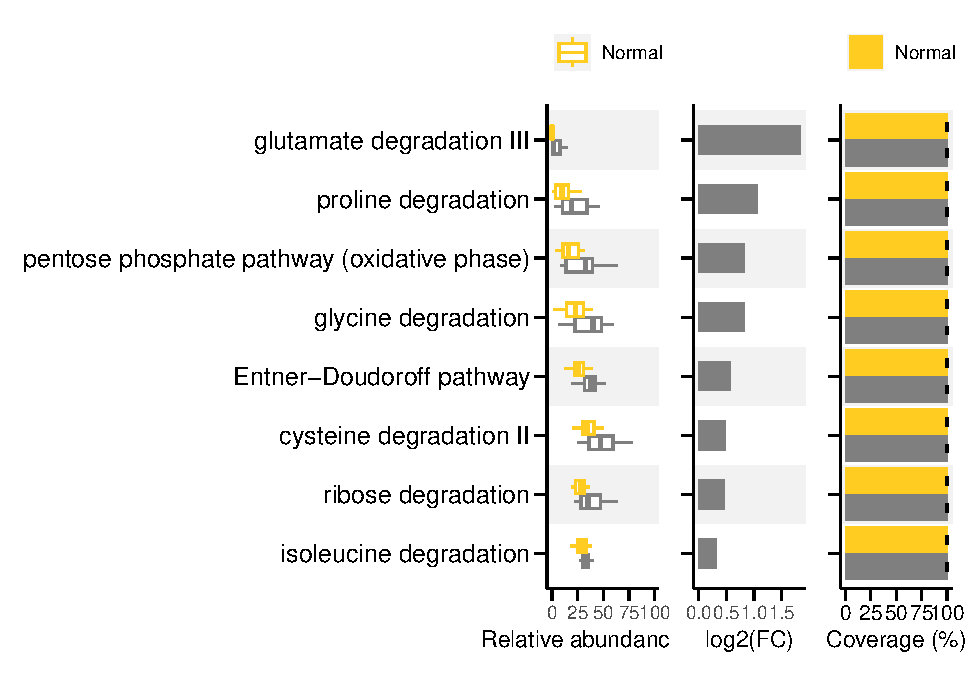
\includegraphics{workshop_files/figure-latex/unnamed-chunk-62-1.pdf}

\hypertarget{co-occurrence-network}{%
\section{Co-Occurrence Network}\label{co-occurrence-network}}

\begin{Shaded}
\begin{Highlighting}[]
\FunctionTok{library}\NormalTok{(Rcpp)}
\FunctionTok{library}\NormalTok{(igraph) }
\FunctionTok{library}\NormalTok{(gtools)}
\FunctionTok{library}\NormalTok{(Matrix)}
\FunctionTok{library}\NormalTok{(SpiecEasi)}
\FunctionTok{sourceCpp}\NormalTok{(}\StringTok{"source/Microbial\_network.cpp"}\NormalTok{)}
\end{Highlighting}
\end{Shaded}

\hypertarget{spiec-easi}{%
\subsection{SPIEC-EASI}\label{spiec-easi}}

\href{https://journals.plos.org/ploscompbiol/article?id=10.1371/journal.pcbi.1004226}{SPIEC-EASI(\textbf{SP}arse
\textbf{I}nvers\textbf{E} \textbf{C}ovariance \textbf{E}stimation for
\textbf{E}cological \textbf{A}ssociation \textbf{I}nference)} infers
direct microbial interactions from compositional data using a graphical
model. It transforms counts into log-ratios, estimates a sparse inverse
covariance matrix with regularization (e.g., Graphical Lasso), and
builds a network where non-zero elements indicate direct species
relationships, overcoming spurious correlations.

\begin{Shaded}
\begin{Highlighting}[]
\NormalTok{pvl\_filter }\OtherTok{\textless{}{-}} \FloatTok{0.1}
\NormalTok{SpiecEasi\_threshold }\OtherTok{\textless{}{-}} \FloatTok{0.7}

\CommentTok{\# filter low prevalence feature}
\NormalTok{pdata }\OtherTok{\textless{}{-}}\NormalTok{ data}
\NormalTok{pdata[pdata }\SpecialCharTok{\textgreater{}} \DecValTok{0}\NormalTok{] }\OtherTok{\textless{}{-}} \DecValTok{1}
\NormalTok{keep\_id }\OtherTok{\textless{}{-}} \FunctionTok{rownames}\NormalTok{(pdata)[}\FunctionTok{rowSums}\NormalTok{(pdata) }\SpecialCharTok{\textgreater{}} \FunctionTok{ncol}\NormalTok{(pdata)}\SpecialCharTok{*}\NormalTok{pvl\_filter]}
\NormalTok{filerted\_data }\OtherTok{\textless{}{-}}\NormalTok{ data[keep\_id,]}
\FunctionTok{dim}\NormalTok{(filerted\_data)}
\DocumentationTok{\#\# [1] 645  40}

\CommentTok{\# run SpiecEas mb = Neighborhood Selection, glasso = graph LASSO}
\NormalTok{SPIEC\_EASI }\OtherTok{\textless{}{-}} \FunctionTok{spiec.easi}\NormalTok{(}\FunctionTok{t}\NormalTok{(filerted\_data), }\AttributeTok{method=}\StringTok{\textquotesingle{}mb\textquotesingle{}}\NormalTok{, }\AttributeTok{lambda.min.ratio=}\FloatTok{1e{-}2}\NormalTok{, }\AttributeTok{nlambda=}\DecValTok{15}\NormalTok{)}
\DocumentationTok{\#\# Applying data transformations...}
\DocumentationTok{\#\# Selecting model with pulsar using stars...}
\DocumentationTok{\#\# Fitting final estimate with mb...}
\DocumentationTok{\#\# done}
\NormalTok{adjm }\OtherTok{\textless{}{-}} \FunctionTok{getOptMerge}\NormalTok{(SPIEC\_EASI)}
\NormalTok{adjm }\OtherTok{\textless{}{-}} \FunctionTok{as.matrix}\NormalTok{(adjm)}
\NormalTok{adjm[adjm }\SpecialCharTok{\textless{}}\NormalTok{ SpiecEasi\_threshold] }\OtherTok{\textless{}{-}} \DecValTok{0}

\NormalTok{edge\_table }\OtherTok{\textless{}{-}} \FunctionTok{make\_edgetable}\NormalTok{(adjm, filerted\_data)}
\NormalTok{node\_table }\OtherTok{\textless{}{-}} \FunctionTok{make\_nodetable}\NormalTok{(edge\_table, data, taxa)}
\end{Highlighting}
\end{Shaded}

\hypertarget{sparcc}{%
\subsection{SparCC}\label{sparcc}}

\href{https://journals.plos.org/ploscompbiol/article?id=10.1371/journal.pcbi.1002687}{SparCC
(\textbf{S}parse \textbf{C}orrelations for \textbf{C}ompositional data)}
infers microbial interactions from compositional data by estimating
correlations while accounting for the sum constraint. It assumes most
species pairs are uncorrelated, uses log-ratio variance to approximate
correlations, and applies a sparse model to focus on strong
relationships. Iterative refinement reduces noise, producing a
correlation network for ecological insights.

\begin{Shaded}
\begin{Highlighting}[]
\NormalTok{pvl\_filter }\OtherTok{\textless{}{-}} \FloatTok{0.1}
\NormalTok{SparCC\_threshold }\OtherTok{\textless{}{-}} \FloatTok{0.3}
\NormalTok{SparCC\_conf\_threshold }\OtherTok{\textless{}{-}} \FloatTok{0.05}

\CommentTok{\# filter low prevalence feature}
\NormalTok{pdata }\OtherTok{\textless{}{-}}\NormalTok{ data}
\NormalTok{pdata[pdata }\SpecialCharTok{\textgreater{}} \DecValTok{0}\NormalTok{] }\OtherTok{\textless{}{-}} \DecValTok{1}
\NormalTok{keep\_id }\OtherTok{\textless{}{-}} \FunctionTok{rownames}\NormalTok{(pdata)[}\FunctionTok{rowSums}\NormalTok{(pdata) }\SpecialCharTok{\textgreater{}} \FunctionTok{ncol}\NormalTok{(pdata)}\SpecialCharTok{*}\NormalTok{pvl\_filter]}
\NormalTok{filerted\_data }\OtherTok{\textless{}{-}}\NormalTok{ data[keep\_id,]}
\FunctionTok{dim}\NormalTok{(filerted\_data)}

\CommentTok{\# run SparCC}
\NormalTok{sparcc\_cor }\OtherTok{\textless{}{-}} \FunctionTok{sparcc}\NormalTok{(}\FunctionTok{t}\NormalTok{(filerted\_data))}
\NormalTok{sparcc\_boost }\OtherTok{\textless{}{-}} \FunctionTok{sparccboot}\NormalTok{(}\FunctionTok{t}\NormalTok{(filerted\_data), }\AttributeTok{R =} \DecValTok{100}\NormalTok{, }\AttributeTok{ncpus =} \DecValTok{10}\NormalTok{)}
\NormalTok{sparcc\_p }\OtherTok{\textless{}{-}} \FunctionTok{pval.sparccboot}\NormalTok{(sparcc\_boost)}
\NormalTok{cors }\OtherTok{\textless{}{-}}\NormalTok{ sparcc\_p}\SpecialCharTok{$}\NormalTok{cors}
\NormalTok{pvals }\OtherTok{\textless{}{-}}\NormalTok{ sparcc\_p}\SpecialCharTok{$}\NormalTok{pvals}

\CommentTok{\# adjacency matrix constructing}
\NormalTok{sparCCpcors }\OtherTok{\textless{}{-}} \FunctionTok{diag}\NormalTok{(}\FloatTok{0.5}\NormalTok{, }\AttributeTok{nrow =} \FunctionTok{dim}\NormalTok{(sparcc\_cor}\SpecialCharTok{$}\NormalTok{Cor)[}\DecValTok{1}\NormalTok{], }\AttributeTok{ncol =} \FunctionTok{dim}\NormalTok{(sparcc\_cor}\SpecialCharTok{$}\NormalTok{Cor)[}\DecValTok{1}\NormalTok{])}
\NormalTok{sparCCpcors[}\FunctionTok{upper.tri}\NormalTok{(sparCCpcors, }\AttributeTok{diag=}\ConstantTok{FALSE}\NormalTok{)] }\OtherTok{\textless{}{-}}\NormalTok{ cors}
\NormalTok{sparCCpcors }\OtherTok{\textless{}{-}}\NormalTok{ sparCCpcors }\SpecialCharTok{+} \FunctionTok{t}\NormalTok{(sparCCpcors)}
\NormalTok{sparCCpval }\OtherTok{\textless{}{-}} \FunctionTok{diag}\NormalTok{(}\FloatTok{0.5}\NormalTok{, }\AttributeTok{nrow =} \FunctionTok{dim}\NormalTok{(sparcc\_cor}\SpecialCharTok{$}\NormalTok{Cor)[}\DecValTok{1}\NormalTok{], }\AttributeTok{ncol =} \FunctionTok{dim}\NormalTok{(sparcc\_cor}\SpecialCharTok{$}\NormalTok{Cor)[}\DecValTok{1}\NormalTok{])}
\NormalTok{sparCCpval[}\FunctionTok{upper.tri}\NormalTok{(sparCCpval, }\AttributeTok{diag=}\ConstantTok{FALSE}\NormalTok{)] }\OtherTok{\textless{}{-}}\NormalTok{ pvals}
\NormalTok{sparCCpval }\OtherTok{\textless{}{-}}\NormalTok{ sparCCpval }\SpecialCharTok{+} \FunctionTok{t}\NormalTok{(sparCCpval)}
\FunctionTok{rownames}\NormalTok{(sparCCpcors) }\OtherTok{\textless{}{-}} \FunctionTok{rownames}\NormalTok{(filerted\_data)}
\FunctionTok{colnames}\NormalTok{(sparCCpcors) }\OtherTok{\textless{}{-}} \FunctionTok{rownames}\NormalTok{(filerted\_data)}
\FunctionTok{rownames}\NormalTok{(sparCCpval) }\OtherTok{\textless{}{-}} \FunctionTok{rownames}\NormalTok{(filerted\_data)}
\FunctionTok{colnames}\NormalTok{(sparCCpval) }\OtherTok{\textless{}{-}} \FunctionTok{rownames}\NormalTok{(filerted\_data)}
\NormalTok{sparCCpcors[}\FunctionTok{abs}\NormalTok{(sparCCpcors) }\SpecialCharTok{\textless{}}\NormalTok{ SparCC\_threshold }\SpecialCharTok{|}\NormalTok{ sparCCpval }\SpecialCharTok{\textgreater{}}\NormalTok{ SparCC\_conf\_threshold] }\OtherTok{=} \DecValTok{0}

\NormalTok{edge\_table }\OtherTok{\textless{}{-}} \FunctionTok{make\_edgetable}\NormalTok{(sparCCpcors, filerted\_data)}
\NormalTok{node\_table }\OtherTok{\textless{}{-}} \FunctionTok{make\_nodetable}\NormalTok{(edge\_table, data, taxa)}
\end{Highlighting}
\end{Shaded}

\hypertarget{cluster-identification}{%
\subsection{Cluster identification}\label{cluster-identification}}

\begin{Shaded}
\begin{Highlighting}[]
\NormalTok{net }\OtherTok{\textless{}{-}} \FunctionTok{make\_net}\NormalTok{(edge\_table)}
\NormalTok{net\_pack }\OtherTok{\textless{}{-}} \FunctionTok{graph\_from\_incidence\_matrix}\NormalTok{(net, }\AttributeTok{mode =} \StringTok{"total"}\NormalTok{, }\AttributeTok{weighted =} \ConstantTok{TRUE}\NormalTok{)}
\CommentTok{\#clustB \textless{}{-} cluster\_edge\_betweenness(net\_pack)}
\NormalTok{clustW }\OtherTok{\textless{}{-}} \FunctionTok{cluster\_walktrap}\NormalTok{(net\_pack)}
\NormalTok{clustL }\OtherTok{\textless{}{-}} \FunctionTok{cluster\_louvain}\NormalTok{(net\_pack)}
\NormalTok{clustG }\OtherTok{\textless{}{-}} \FunctionTok{cluster\_fast\_greedy}\NormalTok{(net\_pack)}
\NormalTok{clustLE }\OtherTok{\textless{}{-}} \FunctionTok{cluster\_leading\_eigen}\NormalTok{(net\_pack)}
\NormalTok{Modularity }\OtherTok{\textless{}{-}} \FunctionTok{data.frame}\NormalTok{(}\AttributeTok{Method =} \FunctionTok{c}\NormalTok{(}\StringTok{"Random walks"}\NormalTok{, }\StringTok{"Louvain"}\NormalTok{, }\StringTok{"Greedy"}\NormalTok{, }\StringTok{"Non{-}negative eigenvector"}\NormalTok{),}
                         \AttributeTok{Modularity =} \FunctionTok{c}\NormalTok{(}\FunctionTok{modularity}\NormalTok{(clustW), }\FunctionTok{modularity}\NormalTok{(clustL),}
                                        \FunctionTok{modularity}\NormalTok{(clustG),}\FunctionTok{modularity}\NormalTok{(clustLE)))}
\NormalTok{Modularity}
\NormalTok{Modul\_number\_cutoff }\OtherTok{\textless{}{-}} \DecValTok{3}  \CommentTok{\# if the number of members in a cluster is lower than the cutoff, discard this cluster.}
\NormalTok{edge\_table }\OtherTok{\textless{}{-}} \FunctionTok{assignModul}\NormalTok{(edge\_table,clustW, }\StringTok{"RandomWalks"}\NormalTok{, Modul\_number\_cutoff)}
\NormalTok{edge\_table }\OtherTok{\textless{}{-}} \FunctionTok{assignModul}\NormalTok{(edge\_table,clustL, }\StringTok{"Louvain"}\NormalTok{, Modul\_number\_cutoff)}
\NormalTok{edge\_table }\OtherTok{\textless{}{-}} \FunctionTok{assignModul}\NormalTok{(edge\_table,clustG, }\StringTok{"Greedy"}\NormalTok{, Modul\_number\_cutoff)}
\NormalTok{edge\_table }\OtherTok{\textless{}{-}} \FunctionTok{assignModul}\NormalTok{(edge\_table,clustLE, }\StringTok{"Leading\_eigen"}\NormalTok{, Modul\_number\_cutoff)}

\FunctionTok{write.csv}\NormalTok{(edge\_table, }\StringTok{"edge\_table.csv"}\NormalTok{, }\AttributeTok{row.names =}\NormalTok{ F,}\AttributeTok{quote =}\NormalTok{ F)}
\FunctionTok{write.csv}\NormalTok{(node\_table, }\StringTok{"node\_table.csv"}\NormalTok{, }\AttributeTok{row.names =}\NormalTok{ F,}\AttributeTok{quote =}\NormalTok{ F)}
\end{Highlighting}
\end{Shaded}

Next, you can visualize with
\href{https://gephi.org/users/download/}{Gephi}.

\hypertarget{guide-to-shotgun-metagenomic-data}{%
\section{Guide to Shotgun Metagenomic
Data}\label{guide-to-shotgun-metagenomic-data}}

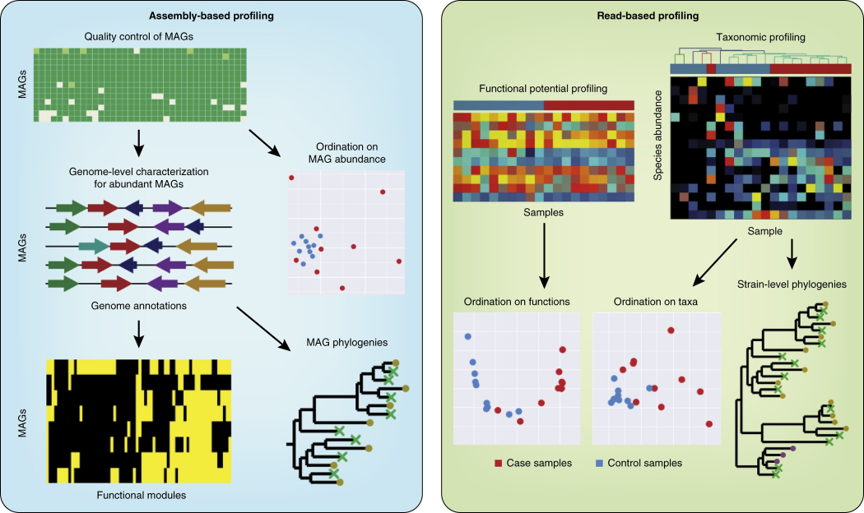
\includegraphics[width=0.8\textwidth,height=\textheight]{images/Fig16.png}

\hypertarget{read-bases-pipeline}{%
\subsection{Read bases pipeline}\label{read-bases-pipeline}}

Shotgun metagenomics involves sequencing all genetic material in a
sample, generating vast amounts of short DNA fragments known as read
bases. These raw reads undergo quality control, filtering, and taxonomic
or functional annotation.

\href{https://huttenhower.sph.harvard.edu/home/}{The Huttenhower Lab}
has developed a comprehensive pipeline called
\texttt{bioBakery\ Workflows}, which includes:

\begin{itemize}
\item
  \textbf{KneadData}: Read quality control and host contamination
  removal
\item
  \textbf{MetaPhlAn}: Taxonomic profiling
\item
  \textbf{HUMAnN}: Functional profiling
\item
  \textbf{PhyloPhlAn}: Phylogenetic analysis
\end{itemize}

Our lab also developed a user friendly \texttt{bioBakery\ Workflows}
named \href{https://github.com/RynoLiu/BacNex}{\texttt{BacNex}}

\begin{Shaded}
\begin{Highlighting}[]
\NormalTok{\# Installation}
\NormalTok{$ git clone https://github.com/RynoLiu/BacNex.git}
\NormalTok{$ conda env create {-}f /env/bacnex\_env\_v2.yml {-}{-}name bacnex\_env}
\NormalTok{$ conda activate bacnex\_env}

\NormalTok{\# Build database}
\NormalTok{$ bash BacNex.sh make\_database {-}o $OUTDIR}

\NormalTok{\# Preprocess (KneadData {-}\textgreater{} MetaPhlAn {-}\textgreater{} HUMAnN)}
\NormalTok{$ bash BacNex.sh preprocess {-}i $seq\_dir \textbackslash{}}
\NormalTok{                            {-}o $outdir \textbackslash{}}
\NormalTok{                            {-}db $DATABASE \textbackslash{}}
\NormalTok{                            {-}{-}threads 10}

\NormalTok{\# Output HUMAnN table}
\NormalTok{$ python BacNex.py make\_table {-}i $KO\_TSV \textbackslash{}}
\NormalTok{                              {-}o $OUTDIR}

\NormalTok{\# shiny APP}
\NormalTok{$ bash BacNex.sh app {-}w $WORK\_DIR \textbackslash{}}
\NormalTok{                     {-}t 10}
\end{Highlighting}
\end{Shaded}

\begin{Shaded}
\begin{Highlighting}[]
\NormalTok{$ git clone https://github.com/RynoLiu/BacNex.git}
\NormalTok{$ conda env create {-}f /env/bacnex\_env\_v2.yml {-}{-}name bacnex\_env}
\NormalTok{$ conda activate bacnex\_env}
\end{Highlighting}
\end{Shaded}

\hypertarget{assembly-bases-pipeline}{%
\subsection{Assembly bases pipeline}\label{assembly-bases-pipeline}}

Assembly bases, on the other hand, refer to contigs or scaffolds
reconstructed from overlapping reads, providing longer genomic sequences
for better functional and phylogenetic analysis.

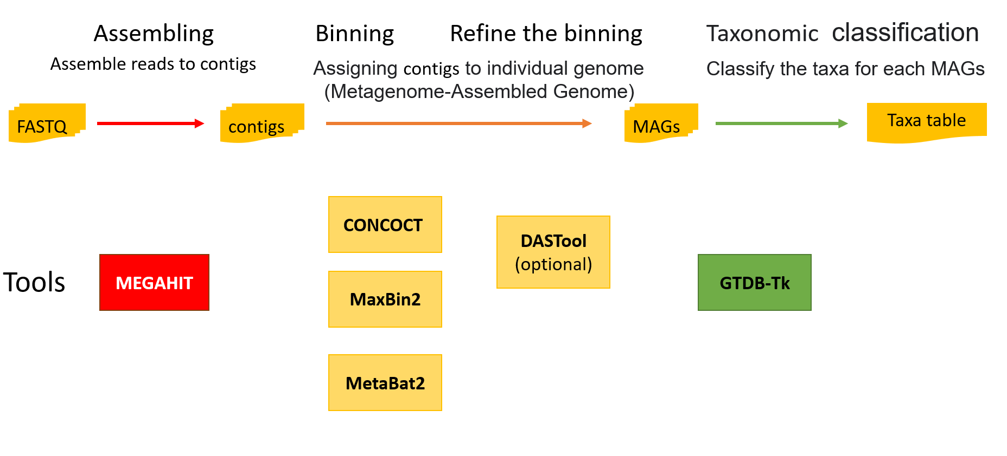
\includegraphics[width=0.8\textwidth,height=\textheight]{images/Fig17.png}

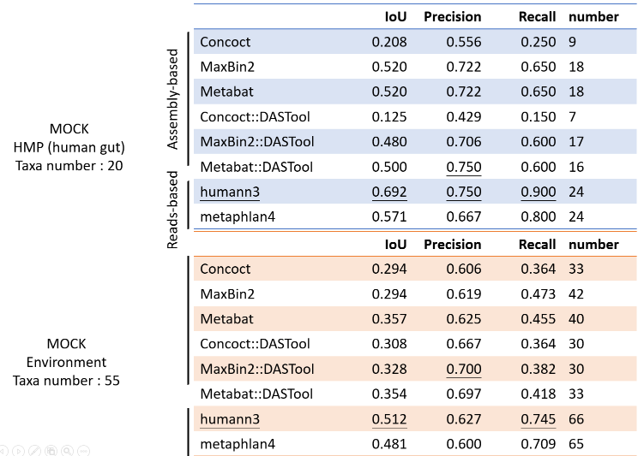
\includegraphics[width=0.8\textwidth,height=\textheight]{images/Fig18.png}

While read-based analysis offers high-resolution species profiling,
assembly-based approaches improve gene prediction and strain-level
characterization. Choosing between them depends on study objectives,
sample complexity, and computational resources.

\end{document}
